\documentclass[12pt]{article}
\usepackage{graphicx} % For including graphics
\usepackage{hyperref} % For URLs and hyperlinks
\usepackage{amsmath} % For math symbols
\usepackage{enumitem} % For customized lists
\usepackage{geometry} % For page margins
\usepackage{xcolor} % For colored text
\usepackage{titlesec} % For title formatting
\usepackage{fancyhdr} % For headers
\usepackage{setspace} % For spacing
\usepackage{graphicx}
\usepackage{gensymb} % For addding degree symbol
\usepackage{multirow}
\usepackage{adjustbox} % For scaling the table
\usepackage{array} % For defining column widths and centering
\usepackage{geometry} % For margin adjustments
\usepackage{booktabs} % For better looking tables
\usepackage{caption}
\usepackage{subcaption}
\usepackage{float}
\usepackage{rotating}      % For sideways tables
\usepackage{tabularx}      % For automatically adjusting column widths
\usepackage{enumitem}      % For controlling list spacing
\usepackage{placeins}  % For \FloatBarrier
\usepackage{caption}
\usepackage{amsmath}
\usepackage{siunitx}
\usepackage[title]{appendix}
\usepackage{pdfpages}

% Page setup
\geometry{a4paper, margin=0.75in} % Adjust margins to allow more space
\setlength{\parindent}{0pt} % Remove indentation
\captionsetup{font=scriptsize}  % Change 'small' to any size: footnotesize, scriptsize, etc.

\setlength{\parskip}{1em} % Adjust spacing between paragraphs
\setlength{\mathindent}{0pt} % Optional: remove extra indent for equations


\renewcommand{\arraystretch}{1.2} % Adjusts the row height

% Title formatting with indentation for sections
% \titleformat{\section}{\bfseries\large\hspace*{1cm}}{\thesection.}{1em}{}
% \titleformat{\subsection}{\bfseries\hspace*{1cm}}{\thesubsection.}{1em}{}
% \titleformat{\subsubsection}{\bfseries\hspace*{2cm}}{\thesubsubsection.}{1em}{}

% Adjust paragraph indentation
\newenvironment{indentedsection}{
    \setlength{\parindent}{1cm} % Indent paragraphs
    \setlength{\leftskip}{1cm} % Indent entire section content
}{}

% Header setup
\pagestyle{fancy}
\fancyhf{}
\fancyhead[L]{Group No: C1}
\fancyhead[C]{ME 407 -- Fall 2024}
\fancyhead[R]{\thepage}

% Horizontal line
\renewcommand{\headrulewidth}{0.4pt}


% Begin Document
\begin{document}

% Main title and keyword section
\begin{center}
    \vspace{1em} % Add some space
    \textbf{\LARGE DETAILED DESIGN}\\
    \vspace{1em} % Add some space
\end{center}

\section{Introduction}

This report encapsulates the finalized decisions and selections; procedures and calculations carried out for the detailed design of the Automatic Table Tennis Ball Pitcher Machine Project. The operating principle of the system, how the system differs from the similar available products on the market, calculations for the functions and the analysis of the system, control algorithms, optimization, manufacturing methods, sustainability analysis, test plans to be carried out, and finally performance analysis and discussion will be laid out clearly. It is important that every one of these steps are documented in detail so that the system is easily and fully understood for any future referencing.

\section{Properties of Designed System}

In this part, properties of the final design will be laid out clearly, where each sub-function will be explained, and the overall operating principle of the system will be given. Important aspects of the design will be discussed, where the applications and functions of the system that differs it from the existing products on the market will be mentioned. Finally, for this part, the machine elements of the system will be considered, and the requirements they bring will be reported.

\subsection{Operating Principle}

The balls are directed to the feeding section from the groove with the help of a channel. The frequency of the balls in the feeding section is adjusted by a Maltese wheel and redirected to the launcher. This Maltese wheel is capable of providing a frequency of up to 60 balls per minute to the system. The system contains a gear pair to adjust the yaw angle and a motor to control the gear pair. These gears are located in a box with bearings enabling the vertical position of the pipe attached to the neck. On the launcher, there is a gear pair controlling the pitch angle, and the motor controlling this gear pair.
This part enables unconstrained movement since it consists of two parts connected by a pin. Finally, the balls reaching the end of the launching part are launched by a 3-wheel system with the desired speed and spin options.  After the launch, the balls are recycled (if they are in the expected region) by a 1 meter high net, back to the storage.  
The device is controlled with an integrated controller and by the potentiometer with buttons located on the controller, the spin, frequency, speed, pitch and yaw angle values are controlled. The device is to be fixed to the table by clamps, and should be stabilized in case of any vibration.

\subsection{Important Aspects of Design}

Although the market for a table tennis ball pitcher machine is not as abundant as some other electronic devices, there are some different designs readily available. The project at hand has to offer some improvements and variations to the existent ideas so it can be marketed as a unique product. 
During a literature survey and market research, it was observed that most commercial products use a rotating head design for launch functions. While this design indeed allows for giving spin to the balls, it also limits how fast the mechanism can switch between different spins, as it requires the head to make a turn beforehand. The design idea in this project utilizes a 3-wheel system for giving the spin, which allows for quicker transition between different spins, ergo allowing for higher frequency.
During the tests, it was found that the wheels attached to the motors for launching are the parts most prone to damage, due to friction and wear during launch. In the design for this project, replacement of the wheels has been facilitated so as to allow for a longer service life, which is an option that has not been come across in any of the other commercial products surveyed.
One limitation the project has is it is fixed at one point on the table. Although it is not a common function in most commercial products, there are some designs that implement flexible movement, so this can be pointed out as a shortcoming compared to those products.

\subsection{Machine Elements and Functional Requirements}

The selection of machine elements is carried out by dividing the entire assembly into smaller subassemblies. Within each subassembly, the choice of machine elements is guided by specific functional requirements, such as ability to withstand loads, accommodate forces, or fit within geometric constraints. This approach ensures that each machine element is selected to meet the demands of its role in the overall design, resulting in effective assembly.


\subsubsection{Launcher}

In the launcher assembly, two socket head screws are used for each motor, totaling six screws. Since these screws are not subjected to any radial load and experience minimal preload, only geometric requirements were considered during their selection. The selected screws are standard M4 socket head screws with a length of 7 mm, chosen according to standard specifications. The design of the launcher is very light-weight and material usage is optimized compared to common products. This is due to using 3 wheel configuration which is controlled with 3 BLDC motors. Without rotating the head part, alternating the speeds of the 3 disks we can give any spin at a desired angle.

\begin{figure}[h!]
    \centering
    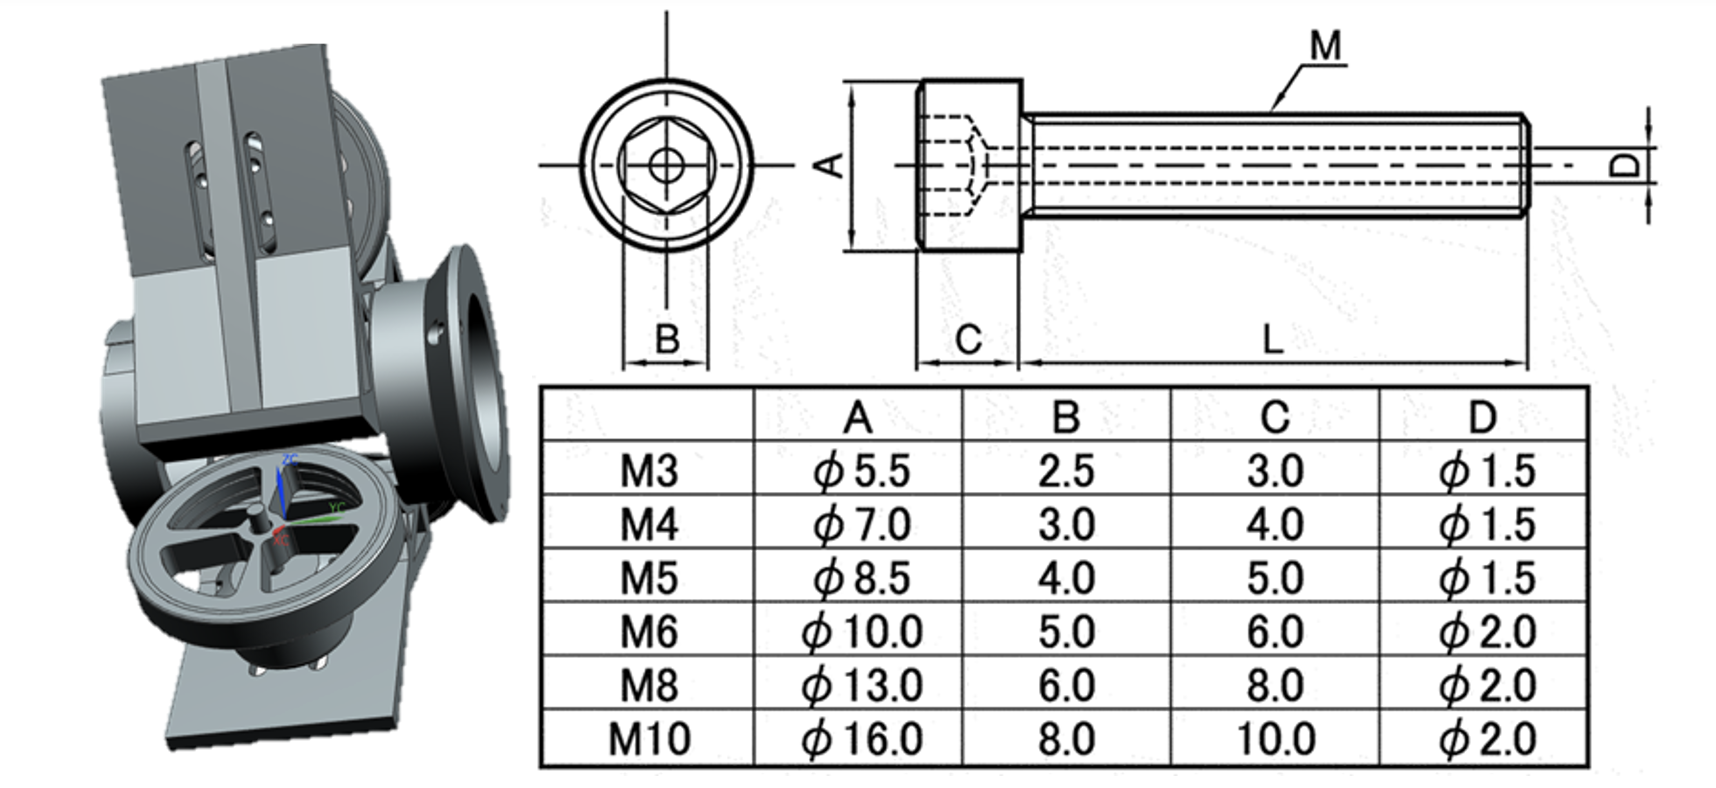
\includegraphics[width=0.7\linewidth]{2.3.1.png}
    \caption{Launcher Subassembly}
    \label{fig:enter-label}
\end{figure}

\subsubsection{Pitch Angle}

The pitch angle subassembly is secured to the launcher using three M3 screws with nuts, each 13 mm in length. For attaching the pitch motor to the pitch angle subassembly, two M3 hex bolts (13 mm) with three nuts are used. To connect the pitch angle subassembly to the main body, four M4 hex bolts (13 mm) with corresponding nuts are utilized. Additionally, the pinion has 17 teeth, while the gear has 65 teeth.

\begin{figure}[h!]
    \centering
    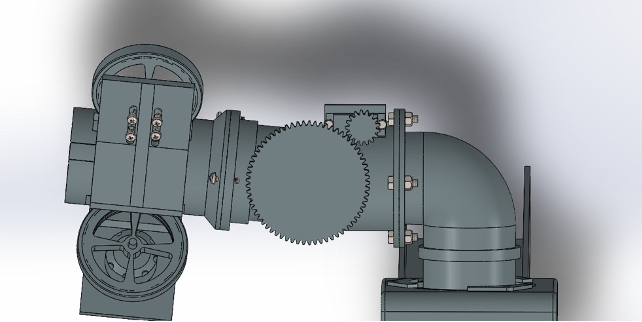
\includegraphics[width=0.7\linewidth]{2.3.2.png}
    \caption{Pitch angle subassembly}
    \label{fig:enter-label}
\end{figure}


\subsubsection{Main Body and Yaw Angle}

The yaw angle assembly in the table tennis ball pitching machine is designed for precise motion control, achieved using a gear pair and bearings. Two SKF 6810 bearings are incorporated based on calculated radial and axial force requirements, ensuring smooth rotation and durability. The bearings are mounted within blind holes in the housing, secured using hex-head M4 screws. Threaded inserts and hex-head screws fasten the main body components.
The assembly integrates a bushing with keys for coupling the driven gear, which includes corresponding keyways to prevent slippage. A servo motor drives this setup, providing precise angular adjustments and smooth acceleration. A 0.45 gear ratio is selected to enhance yaw angle control accuracy.
This design rotates the system's feeding line rather than the launcher head directly, offering multiple advantages:

\begin{enumerate}
    \item Compact launcher design.
    \item Reduced stress on the launcher components.
    \item Simplified assembly and disassembly.
\end{enumerate}

The spur gear pair minimizes axial load, while the feeding line, shrink-fitted into two bearings at either end of the main body, ensures optimized reliability. The upper part of the feeding system is isolated from the pipe, ensuring only the top section rotates, which requires the launcher components to remain lightweight for efficient operation.

\begin{figure}[h!]
    \centering
    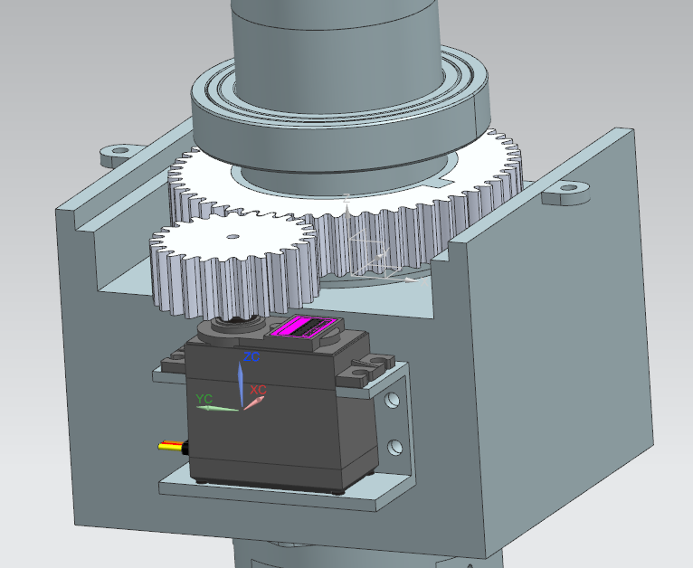
\includegraphics[width=0.5\linewidth]{2.3.3.1.png}
    \caption{Yaw angle subassembly}
    \label{fig:enter-label}
\end{figure}

\begin{figure}[h!]
    \centering
    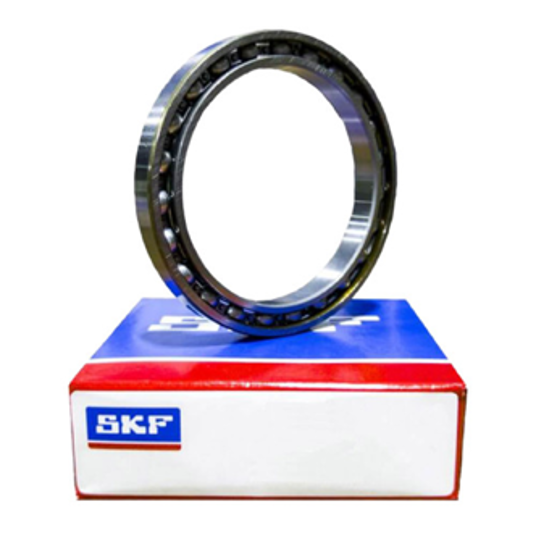
\includegraphics[width=0.3\linewidth]{2.3.3.2.png}
    \caption{6810 ZZ Bearing}
    \label{fig:enter-label}
\end{figure}

\begin{table}[h!]
\scriptsize
\centering
\caption{Yaw angle components}
\begin{tabular}{|c|p{9cm}|}
\hline
\textbf{Component} & \textbf{Properties} \\ \hline
Driving Gear & Spur Gear, Module 1.5, Teeth Number 25 \\ \hline
Driven Gear & Spur Gear, Module 1.5, Teeth Number 55, Keyway slotted \\ \hline
Motor & MG996R Servo Motor \\ \hline
Bushing & Manufactured with keys, Shrink fit \\ \hline
Bearings & NSK 6910 ZZ Ball Bearing, High load and fatigue capacity, Shrink fit \\ \hline
Feeding Line & 50mm diameter pipe, Shrink fit \\ \hline
\end{tabular}
\label{table:yaw_components}
\end{table}


\subsubsection{Feeding Mechanism}
The feeding mechanism incorporates a Maltese wheel designed for continuous ball delivery to the launcher. The wheel is driven by a stepper motor, with each 60-degree rotation feeding one ball. This setup allows precise control over the number of balls to be launched.
The feeding pipe is tightly secured to the feeding holder using an H6/e6 interference fit. The connection is further reinforced with four M3 set screws, each 3 mm in length, a method commonly used in prosthetic applications for its reliability. The feeding holder is attached to the main body using M4 bolts and threaded inserts, providing a factor of safety of approximately 3.8.
This design is highly compatible with the ball recycling system, ensuring efficient operation. However, a notable drawback is the increased space requirement for the feeding pipe.

\begin{figure}[h!]
    \centering
    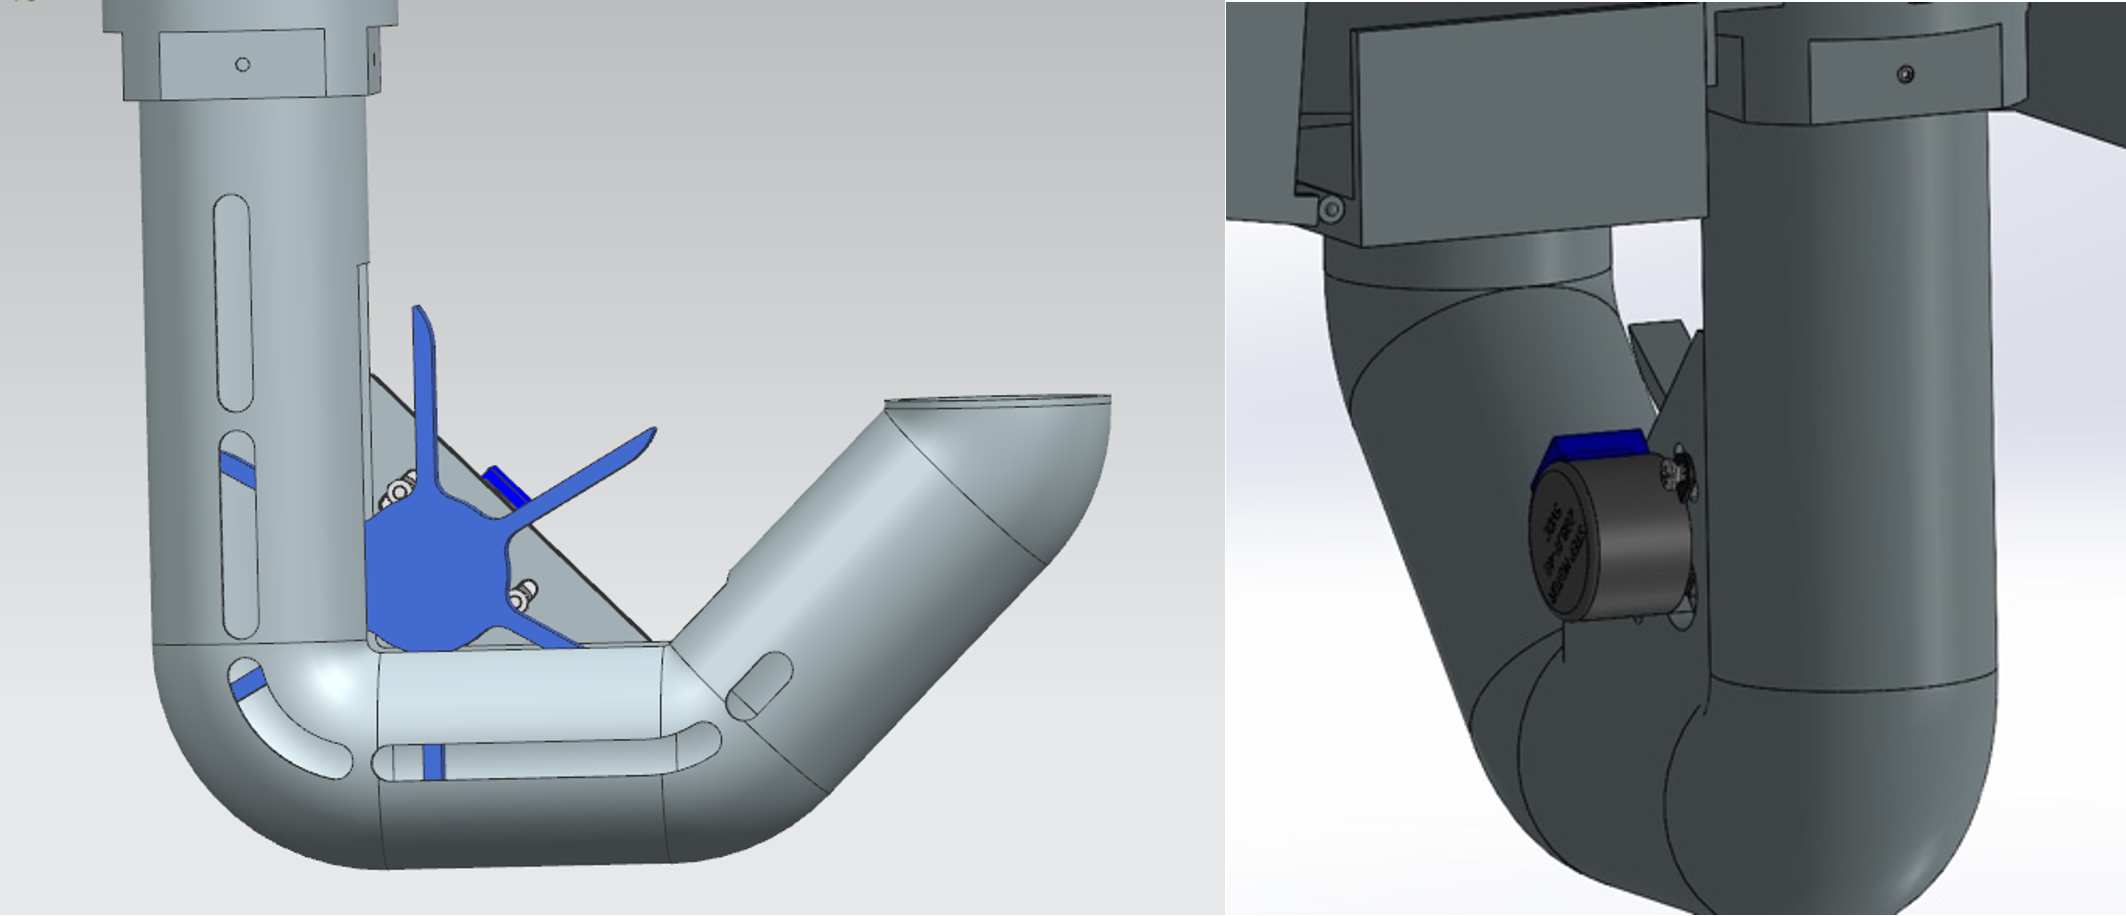
\includegraphics[width=0.7\linewidth]{2.3.4.1.png}
    \caption{Feeding system subassembly}
    \label{fig:enter-label}
\end{figure}

\begin{figure}[h!]
    \centering
    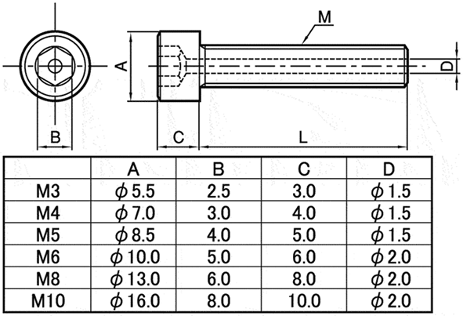
\includegraphics[width=0.5\linewidth]{2.3.4.2.png}
    \caption{Socket head bolt}
    \label{fig:enter-label}
\end{figure}

\begin{figure}[h!]
    \centering
    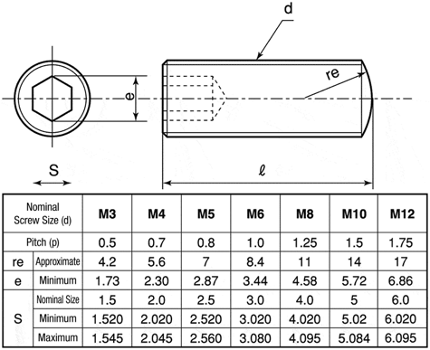
\includegraphics[width=0.5\linewidth]{2.3.4.3.png}
    \caption{Set screw}
    \label{fig:enter-label}
\end{figure}

\begin{table}[h!]
\scriptsize
\centering
\caption{Feeding system components}
\begin{tabular}{|c|p{6cm}|}
\hline
\textbf{Component} & \textbf{Properties} \\ \hline
Maltese Wheel & 6 slots, ABS \\ \hline
Pipe & 50 mm outside diameter ABS \\ \hline
Motor & Nema17 Step Motor \\ \hline
Bolts and Nuts & M4, Stainless Steel \\ \hline
Set Screws & 3mm length, Nylon tip, Alloy Steel \\ \hline
\end{tabular}
\label{table:feeding_components}
\end{table}


\subsubsection{Ball Recyclability}

A net is used to catch the balls and is complemented by grooves attached to both sides of the robot. The net directs the caught balls into the grooves, allowing them to roll down into the storage unit. The grooves serve as guides, ensuring the balls are efficiently funneled into the storage area. The net is securely connected to the grooves and anchored to the table for stability.

\begin{figure}[h!]
    \centering
    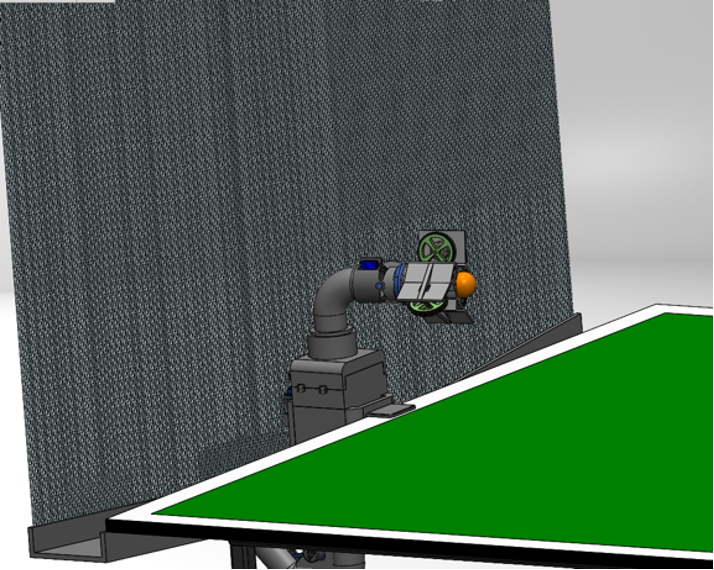
\includegraphics[width=0.5\linewidth]{2.3.5.1.png}
    \caption{Ball Recyclability system}
    \label{fig:enter-label}
\end{figure}

\subsubsection{Storage and Groove}

The grooves are attached to the storage unit using hinges, allowing them to fold for enhanced portability. The connection between the storage unit and the grooves is achieved with welded hinges, as illustrated in the accompanying figure. To secure the storage unit to the main body, four L-plates are utilized. These plates are fastened using M4 bolts (13 mm in length) and nuts, ensuring a stable and reliable connection.

\begin{figure}[h!]
    \centering
    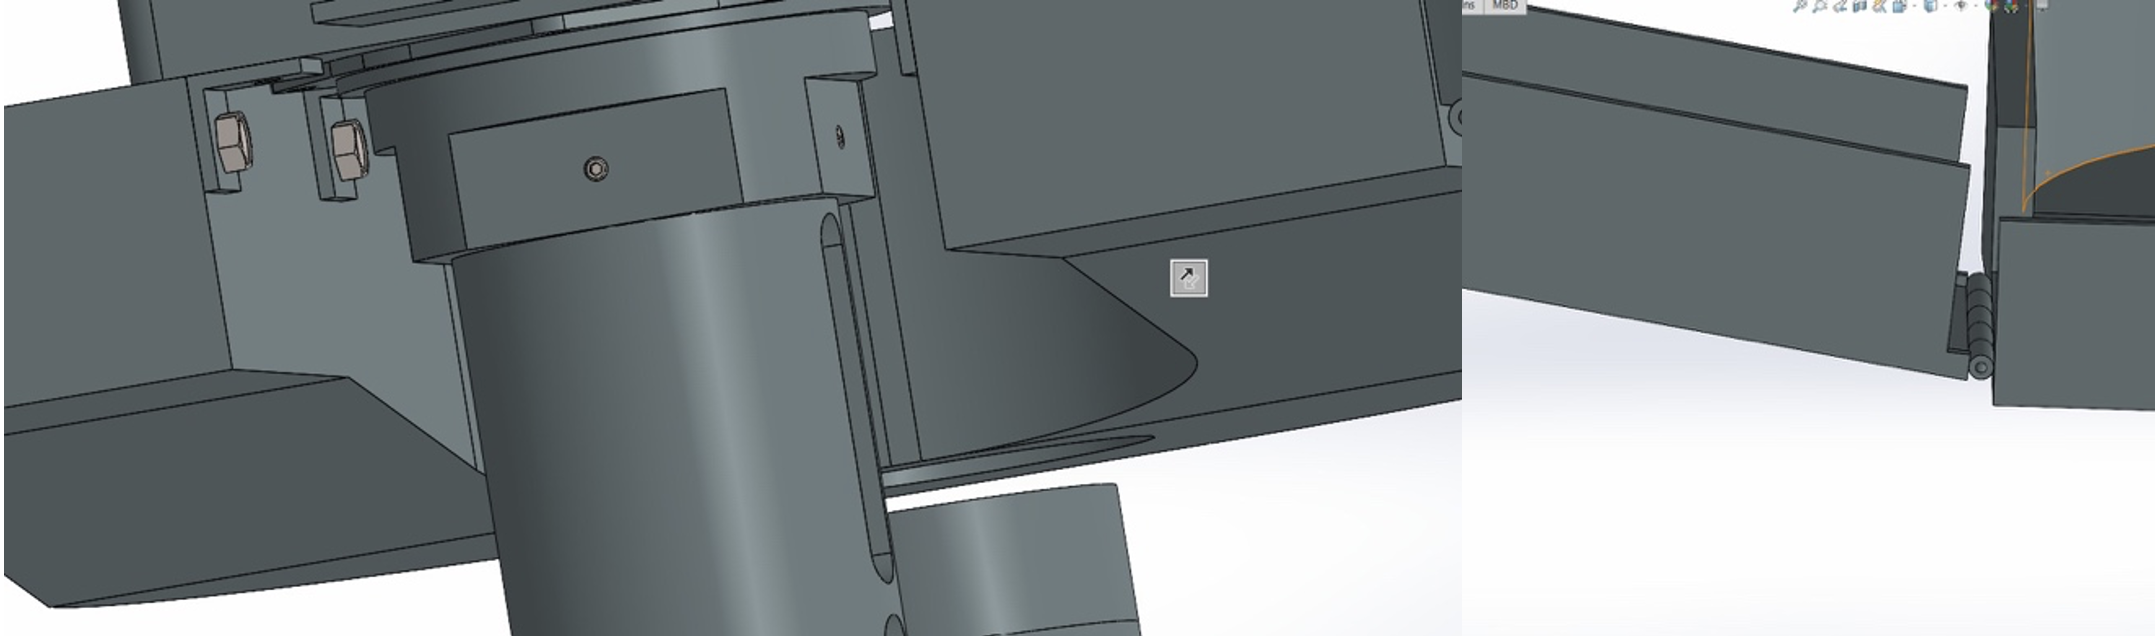
\includegraphics[width=0.5\linewidth]{2.3.6.1.png}
    \caption{Storage system subassembly}
    \label{fig:enter-label}
\end{figure}

\subsubsection{Mounting}

The clamp is specifically designed to support the entire weight of the system. Calculations indicate that the primary factor influencing clamp performance is not the system's weight but the pretension of the clamping screw. To ensure secure attachment, the minimum clamping distance is set to 18 mm, matching the thickness of a standard table.
The clamp is connected to the main body using M5 steel bolts and brass threaded inserts, chosen for their availability and chemical compatibility. To optimize load distribution and stability, four bolts are arranged in a rectangular pattern, providing a firm and reliable fixation.

\begin{figure}[h!]
    \centering
    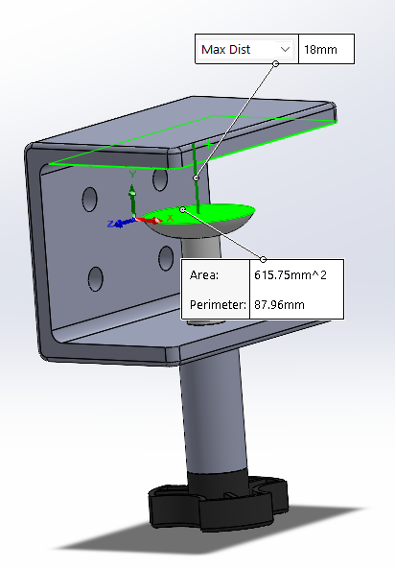
\includegraphics[width=0.3\linewidth]{2.3.7.1.png}
    \caption{Clamp}
    \label{fig:enter-label}
\end{figure}


\section{Engineering Calculations}

This section outlines the essential engineering calculations for the Table Tennis Ball Pitcher Machine, covering areas such as material strength, kinematics, dynamics, and force analysis. Assumptions, modeling simplifications, and approximations are clearly stated to ensure clarity and precision. The calculations validate the performance, safety, and reliability of the design, ensuring it meets the specified requirements. 
The calculations and design decisions can be divided into two main parts:

\subsection{Decisions based on meeting the performance criteria target}

In that section, the decisions based on meeting the performance criteria targets are presented. The type of modelling, the related component of the system, the design parameters to be decided, and the explanations including the assumptions and approximations, the methods or any aid of commercial software are explained in detail.

The table shows the planned models, analyses, and tests to ensure the system meets the required performance standards. For each part or subsystem, it describes the modeling type (analytical, numerical, or experimental), important design factors, and key methods used. It also explains assumptions, like slip percentage and operating conditions, and lists tools such as MATLAB/Simulink, Siemens NX, and Python for simulations and optimization. Table includes motor torque and speed modeling, control strategy simulations, optimizing disk dimensions, and testing materials for the launcher. 

\begin{table}[H]
\centering
\caption{Decisions based on meeting the performance criteria target (Part 1)}
\scriptsize % Reduced font size for the entire table
\renewcommand{\arraystretch}{1.5}
\setlength{\tabcolsep}{4pt}
\begin{tabular}{|>{\raggedright\arraybackslash}p{3cm}|>{\raggedright\arraybackslash}p{3cm}|>{\raggedright\arraybackslash}p{3cm}|>{\raggedright\arraybackslash}p{6cm}|}
\hline
\textbf{Analytical Modelling / Numerical Modelling / Numerical Experiment / Physical Experiment} & \textbf{Component / Subsystem / Whole System} & \textbf{Design Parameters to be Decided} & \textbf{Explanation (State assumptions, any commercial software for the implementation, and details of methods like DoE, optimization etc.)} \\ \hline
Numerical Modelling & Launch Motors & Motor Type, Torque, Speed & Torque and speed requirements for launching wheels will be calculated to achieve a maximum ball speed of 30 m/s. Also, a simulation in Python can be used to model motor torque, angular speed, and efficiency based on required ball velocities and spin. The assumed slip is 20\%. \\ \hline
Numerical Experiment & Launch Motors & Motor Control Strategy & Motor response and speed control for spin adjustments will be simulated. BLDC/DC motors will be controlled via Pulse Width Modulation (PWM) using MATLAB/Simulink for precision. Optimization of spin will ensure accuracy for 36 spin types. \\ \hline
Numerical Modelling & Launch Motors Mounting & Mounting Method, Fasteners & Test motor fixation methods (bolts, clamps) for rigidity and vibration resistance under operation. \\ \hline
Analytical Modelling & Launching Mechanism & Design of Launcher & Siemens NX is used for design. In design small subparts are designed for easy assembly to form a 3-wheeled launcher design. \\ \hline
Physical Experiment & Disk Cover Material & Selection and Implementation of Disk Cover Material & Material selection for the coverage of the disk is a trial and error process. \\ \hline
Numerical Modelling & Disks for Launching & Disk Dimensions & Numerical analysis will be conducted to optimize disk dimensions (diameter and thickness) to achieve the required ball velocity (4--25 m/s) and spin. Will consider stresses, deformation, and rotational inertia of the disks under high rotational speeds (up to 9550--11460 RPM). \\ \hline
\end{tabular}
\label{tab:performance_criteria}
\end{table}


\subsubsection{Launcher Calculations}

In order to check whether our motors at launcher head are capable of reaching specific speeds for giving desired speed and spin to the balls, we will conduct a kinematic analysis.

\begin{figure}[h!]
    \centering
    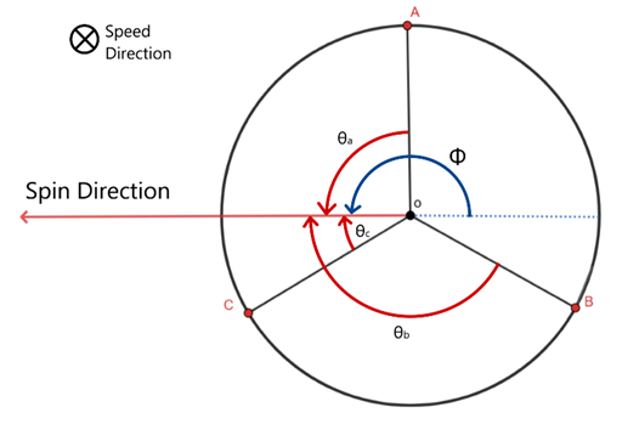
\includegraphics[width=0.4\linewidth]{3.1.1.png}
    \caption{FBD of launcher subassembly}
    \label{fig:enter-label}
\end{figure}

The three wheels in our launcher head are indicated as A, B, and C points in the free body diagram.  Combining linear speed of the ball and point speeds on the surface of contact, derived from the spin speed and spin direction, we can reach the total speed to be achieved at contact points on the surface.

\begin{align}
    V_a &= V + \omega \cdot r \cdot \sin(\theta_a) \\[-0.5pt]
    V_b &= V - \omega \cdot r \cdot \sin(\theta_b) \\[-0.5pt]
    V_c &= V - \omega \cdot r \cdot \sin(\theta_c)
\end{align}

Where V is the desired linear speed of the ball, r is the radius of the ball, and w is desired spin.
The required wheel speeds are calculated as:

\begin{align}
    \omega_a &= \left( \frac{V_a}{r_{\text{wheel}} \cdot \frac{2\pi}{60}} \right) \cdot s \\[-0.5pt]
    \omega_b &= \left( \frac{V_b}{r_{\text{wheel}} \cdot \frac{2\pi}{60}} \right) \cdot s \\[-0.5pt]
    \omega_c &= \left( \frac{V_c}{r_{\text{wheel}} \cdot \frac{2\pi}{60}} \right) \cdot s
\end{align}



Where s is the slip amount.
For the limiting condition with V=30 m/s and assuming 20\% slip amount, a maximum rotation speed of 12000 rpm is needed in the motors. For that 2300 KV BLDC motors are selected, which can reach speeds of up to 15000-20000 rpm.
There are assumptions and approximations in these calculations. So, the real-life scenario may not exactly reflect the calculation results. These assumptions are about neglecting the effect of wheel mass on rotation speed, determining slip ratio, motor speed accuracy, and squeezing amount of ball. In order to form the relation between calculation results and real-life results, calibration experiments should be done.

The table 4 shows the planned models, analyses, and tests to ensure the system meets the required performance standards. For each part or subsystem, it describes the modeling type (analytical, numerical, or experimental), important design factors, and key methods used. For example, numerical simulations with Siemens NX will be used to optimize gear ratios and motor performance for the yaw and pitch angle motors, while physical experiments will validate the stability and responsiveness of the motor and gear systems. Additionally, tools like SKF catalogs and gear analysis software will assist in selecting appropriate bearings and calculating gear dimensions.


\begin{table}[H]
\centering
\caption{Decisions based on meeting the performance criteria target (Part 2)}
\scriptsize % Adjust font size if needed (e.g., \small, \scriptsize, \tiny)
\renewcommand{\arraystretch}{1.5}
\setlength{\tabcolsep}{4pt}
\begin{tabular}{|>{\raggedright\arraybackslash}p{4cm}|>{\raggedright\arraybackslash}p{3cm}|>{\raggedright\arraybackslash}p{3cm}|>{\raggedright\arraybackslash}p{6cm}|}
\hline
\textbf{Analytical Modelling / Numerical Modelling / Numerical Experiment / Physical Experiment} & \textbf{Component / Subsystem / Whole System} & \textbf{Design Parameters to be Decided} & \textbf{Explanation)} \\ \hline
Numerical Modelling & Yaw Angle Motor & Gear Ratio, Torque, Accuracy & Motor selection for yaw angle control will consider torque and speed requirements using a model of gears. Simulations with Siemens NX will optimize motor and gear ratios. \\ \hline
Numerical Experiment & Yaw Angle Motor & Control Method, Speed & Accuracy and speed of motor-controlled yaw adjustments will be numerically tested. Servo or stepper motors with feedback control (PID tuning) will be implemented for $-20^\circ$
 to $+20^\circ$° yaw angle precision. \\ \hline
Numerical Modelling & Yaw Angle Gear Pairs & Gear Dimensions & Gear analysis tool in Siemens NX can be utilized. \\ \hline
Analytical Modelling & Bearing of Yaw Angle & Bearing Dimensions & Bearing selection is done based on the SKF catalog. In this case, axial load is higher than radial load. Based on this, appropriate loads are implemented, and the life of the bearing is obtained. \\ \hline
Numerical Modelling & Pitch Angle Motor & Gear System, Required Torque & Pitch angle adjustments ($-20^\circ$
 to $+20^\circ$) required torque and speed will be calculated. The gear system controlled by servos will be numerically simulated for precise angle control. \\ \hline
Physical Experiment & Pitch Angle Motor & Stability, Responsiveness & Physical testing of motor and gear mechanisms for pitch angle adjustments will ensure smooth and reliable operation. Experiments will validate the responsiveness of worm and bevel gear systems to dynamic pitch commands. \\ \hline
Analytical Modelling & Pitch Angle Gear Pairs & Gear Dimensions & Gear analysis tool in Siemens NX can be utilized. \\ \hline
\end{tabular}
\label{tab:performance_criteria}
\end{table}



\subsubsection{Yaw Angle Calculations}

For checking whether the motor is suitable to meet the performance criteria, the stall torque supplied by the motor will be considered. For the relation, the work done by the system will be calculated and compared with the work done by the motor. For the calculation, the loss due to the friction inside the motor was assumed negligible as both the friction factor and the angular velocity assumed were very small. So, the main factor contributing to the work were the moments of inertia of the components. Proceeding with the calculations,

\textbf{Head Inertia:}
\begin{align}
I_\text{head} = \frac{1}{12} \cdot 0.25 \cdot \left(0.06^2 + 0.15^2\right) + 0.125^2 \cdot 0.25
\end{align}

\begin{align}
I_\text{head} = 4.45 \cdot 10^{-3}\ \si{\kilogram\meter\squared}
\end{align}

\textbf{Pipe 1 Inertia:}
\begin{align}
I_\text{pipe1} &= \frac{1}{12} \cdot 0.075 \cdot \left[ 3 \cdot \left( \left(\frac{0.43}{2}\right)^2 + \left(\frac{0.05}{2}\right)^2 \right) + 0.095^2 \right] + 0.075 \cdot 0.05^2
\\
I_\text{pipe1} &= 2.64 \cdot 10^{-4}
\end{align}

\textbf{Pipe 2 Inertia:}
\begin{align}
I_\text{pipe2} &= \frac{1}{2} \cdot 0.075 \cdot \left[ \left(\frac{0.043}{2}\right)^2 + \left(\frac{0.05}{2}\right)^2 \right]
\\
I_\text{pipe2} &= 4.077 \cdot 10^{-5}
\end{align}

\textbf{Total Inertia:}
\begin{align}
I_\text{total} = 4.57 \cdot 10^{-3}\ \si{\kilogram\meter\squared}
\end{align}

Taking angular velocity \(\omega = 3.14\ \si{\radian\per\second}\),

\textbf{Kinetic Energy:}
\begin{align}
E_k = \frac{1}{2} \cdot I \cdot \omega^2 = 0.02\ \si{\joule}
\end{align}

For a \(40^\circ\) rotation, \(t = 0.22\ \si{\second}\),

\textbf{Power:}
\begin{align}
P = \frac{E_k}{t} = 0.09\ \si{\watt}
\end{align}

Assuming a reduction of 2 between gears, \(\omega_\text{motor} = 6.28\ \si{\radian\per\second}\),

The stall torque of the motor is \(2.2\ \si{\kilogramf\centi\meter}\), thus:

\begin{align}
0.0216\ \si{\newton\meter} \cdot 6.28\ \si{\radian\per\second} = 0.136\ \si{\watt} > 0.09\ \si{\watt}
\end{align}

It can be seen that the supplied torque by the motor is enough to meet the requirement.

\subsubsection{Pitch Angle Calculations}

For pitch angle the same motor is used, and the method will be the same. Proceeding with the same assumptions, the main factor contributing to work on the system part for this case was found to be the potential energy change between the configurations when the head is at its uppermost and lowermost position. Thus,

From the law of cosines:
\begin{align}
0.07^2 \cdot 2 - 0.07^2 \cdot \cos(40^\circ) &= 6.05 \cdot 10^{-3}\ \si{\meter}
\end{align}

\textbf{Potential Energy:}
\begin{align}
E_p &= 9.81 \cdot 0.25 \cdot 6.05 \cdot 10^{-3} \\
E_p &= 0.01\ \si{\joule}
\end{align}

For \(\omega = 1.57\ \si{\radian\per\second}\), a \(40^\circ\) pitch angle gives \(t = 0.44\ \si{\second}\):

\textbf{Power:}
\begin{align}
P &= \frac{E_p}{t} \\
P &= 0.02\ \si{\watt}
\end{align}

\textbf{Motor Calculations:}  
Assuming a reduction ratio of 2, \(\omega_\text{motor} = 3.14\ \si{\radian\per\second}\).  
The stall torque of the motor is \(2.2\ \si{\kilogramf\centi\meter}\), thus:
\begin{align}
0.0216\ \si{\newton\meter} \cdot 3.14\ \si{\radian\per\second} &= 0.068\ \si{\watt} > 0.02\ \si{\watt}
\end{align}

It can again be seen that the supplied torque by the motor is suitable for the fulfilling of the requirement.

\subsubsection{Gear Calculations}

\begin{table}[ht]
\centering
\renewcommand{\arraystretch}{1.5}
\setlength{\tabcolsep}{10pt}
\begin{tabular}{>{\raggedright\arraybackslash}p{5cm} >{\raggedright\arraybackslash}p{8cm}}
\textbf{Parameter}          & \textbf{Value and Calculation} \\ 
Pressure angle              & $\alpha = 20^\circ$ \\ 
Module                     & $m = 1$ \\ 
Number of teeth             & $z = 65$ \\ 
Pitch circle diameter       & $d_o = m \cdot z = 1 \cdot 65 = 65\ \text{mm}$ \\ 
Addendum circle diameter    & $d_a = d_o + 2 \cdot m = 65 + 2 \cdot 1 = 67\ \text{mm}$ \\ 
Dedendum circle diameter    & $d_f = d_o - 2.5 \cdot m = 65 - 2.5 \cdot 1 = 62.5\ \text{mm}$ \\ 
Face width                  & $b = 10 \cdot m = 10 \cdot 1 = 10\ \text{mm}$ \\ 
Working depth               & $h = 2.166 \cdot m = 2.166 \cdot 1 = 2.17\ \text{mm}$ \\ 
Addendum                    & $h_a = m = 1\ \text{mm}$ \\ 
Dedendum                    & $h_f = h - h_a = 2.17 - 1 = 1.17\ \text{mm}$ \\ 
Design angle                & $\alpha = \frac{180}{z} = \frac{180}{65} = 2.77^\circ$ \\ 
\end{tabular}
\label{tab:gear_parameters}
\end{table}
\newpage

A table demonstrating the calculated values of gear and pinion of pitch and yaw angle is presented below.

\begin{table}[H]
\centering
\caption{Gear dimensions}
\begin{tabular}{|c|c|c|c|c|}
\hline
\textbf{Parameter} & \textbf{Yaw Pinion} & \textbf{Yaw Gear} & \textbf{Pitch Pinion} & \textbf{Pitch Gear} \\ \hline
$m$ (Module)       & 1.5                 & 1.5               & 1                     & 1                   \\ \hline
$z$ (Teeth Number) & 25                  & 55                & 17                    & 65                  \\ \hline
$d_o$ (mm)         & 37.5                & 82.5              & 17                    & 65                  \\ \hline
$d_a$ (mm)         & 40.5                & 85.5              & 19                    & 67                  \\ \hline
$d_f$ (mm)         & 33.75               & 78.75             & 14.5                  & 62.5                \\ \hline
$b$ (mm)           & 15                  & 15                & 10                    & 10                  \\ \hline
$h$ (mm)           & 3.25                & 3.25              & 2.17                  & 2.17                \\ \hline
$h_a$ (mm)         & 1.5                 & 1.5               & 1                     & 1                   \\ \hline
$h_f$ (mm)         & 1.75                & 1.75              & 1.17                  & 1.17                \\ \hline
$a$ (°)            & 7.2                 & 3.27              & 10.59                 & 2.77                \\ \hline
\end{tabular}
\label{table:gear_dimensions}
\end{table}

\begin{figure}[h!]
    \centering
    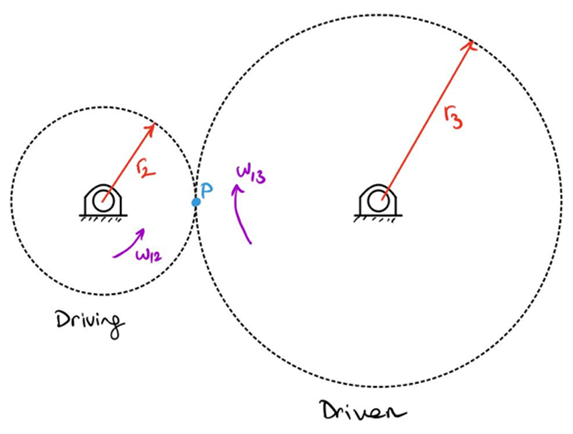
\includegraphics[width=0.5\textwidth]{fig12 gear kin.png} 
    \caption{Gear kinematics} 
    \label{Gear Kinematics} 
\end{figure}

Yaw Angle
\begin{align}
    R_{23} &= \frac{\omega_{13}}{\omega_{12}} = -\frac{r_2}{r_3} \\
    R_{23} &= -\frac{25}{55} = -0.45
\end{align}
\begin{align}
    \omega_{13} = -0.45 \cdot \omega_{12}
\end{align}


Gear ratio is adjusted such that the yaw angle control is precise. The constraint equation is:
\begin{align}
r_2 \cdot \theta_{12} = -r_3 \cdot (\theta_{13} - \beta_3)
\end{align}
For yaw adjustment:
\begin{align}
    \theta_{13} = -0.45 \cdot \theta_{12} + \beta_3
\end{align}

Special case:
\begin{align}
\text{When } \theta_{12} = 0, \; \beta_3 = \theta_{13}
\end{align}

Pitch Angle

Similar to yaw angle calculations. This time the pinion (driving) is 4, and the gear is 5.

\begin{align}
R_{45} = \frac{\omega_{15}}{\omega_{14}} = -\frac{r_4}{r_5}
\end{align}
\begin{align}
R_{45} = -\frac{17}{65} = -0.262
\end{align}
\begin{align}
\omega_{15} = -0.262 \cdot \omega_{14}
\end{align}

Gear ratio is adjusted such that the pitch angle control is precise. The constraint equation is:
\begin{align}
r_4 \cdot \theta_{14} = -r_5 \cdot (\theta_{15} - \beta_5)
\end{align}
For pitch adjustment:
\begin{align}
\theta_{15} = -0.262 \cdot \theta_{14} + \beta_5
\end{align}
Special case:
\begin{align}
\text{When } \theta_{14} = 0, \; \beta_5 = \theta_{15}
\end{align}

Pitch angle gear ratio is even smaller since more torque output is required, and more precise control is needed for the given design.


\subsubsection{Bearing Calculations}

For the bearing selection, axial and radial loads are exaggerated to be on the safe side. Axial and radial loads are 10 kg and 5 kg respectively. With these assumptions, an iterative process is applied to select a suitable rolling bearing.

Assumed Force Applied to Bearings:

Load:
\begin{align}
    m_{a_{\text{load}}} &= 10 \, \mathrm{kg}, \quad m_{r_{\text{load}}} = 5 \, \mathrm{kg}
\end{align}
Axial Force: 
\begin{align}
    F_a &= m_{a_{\text{load}}} \cdot g = 10 \, \mathrm{kg} \cdot 9.81 \, \mathrm{m/s^2} = 98.1 \, \mathrm{N}
\end{align}
Radial Force: 
\begin{align}
    F_r &= m_{r_{\text{load}}} \cdot g = 5 \, \mathrm{kg} \cdot 9.81 \, \mathrm{m/s^2} = 49.05 \, \mathrm{N}
\end{align}

Dynamic Bearing Load:
\begin{align}
    P &= X \cdot F_r + Y \cdot F_a
\end{align}


\[
P = \text{equivalent dynamic bearing load} \, [\mathrm{kN}]
\]
\[
F_r = \text{actual radial bearing load} \, [\mathrm{kN}]
\]
\[
F_a = \text{actual axial bearing load} \, [\mathrm{kN}]
\]
\[
X = \text{radial load factor for the bearing}
\]
\[
Y = \text{axial load factor for the bearing}
\]


\begin{figure}[h]
    \centering
    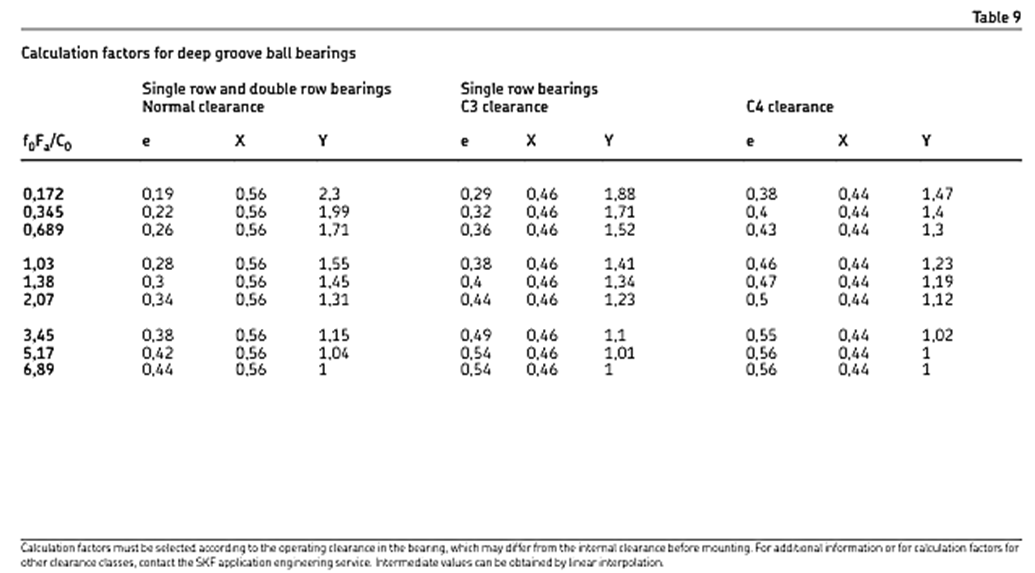
\includegraphics[width=0.8\linewidth]{bearingfactors.png}
    \caption{Calculation factors for deep groove ball bearings}
    \label{fig:bearingfactors}
\end{figure}

\begin{align}
\frac{f_o \cdot F_a}{C_o} = 0.25
\end{align}
\begin{align}
e = 0.25
\end{align}
\begin{align}
X=0.56
\end{align}
\begin{align}
Y=2.145
\end{align}
\begin{align}
P=0.2425  \,\mathrm{kN}
\end{align}

Properties

Rotational Speed \begin{align}
n = 40 \, \text{deg/s} = 6.67 \, \text{rpm}
\end{align}
The angular velocity is determined based on the requirements for the yaw angle adjustment. The yaw angle must be adjustable within a range of -20° to +20°. Consequently, it is specified that the bearing mechanism should accommodate 40° of angular motion per second, corresponding to an angular velocity of approximately 6.67 rpm.	

Mean Diameter
\begin{align}
d_m = \frac{d + D}{2} = \frac{50 + 65}{2} = 57.5 \, \mathrm{mm}
\end{align}

The mean diameter is calculated as the average of the internal and external diameters. In our design, the internal diameter is specified as 50 mm. Accordingly, the external diameter is selected as the smallest available diameter from the catalog, which is 65 mm.

Rated Viscosity Estimation

\begin{figure}[h!]
    \centering
    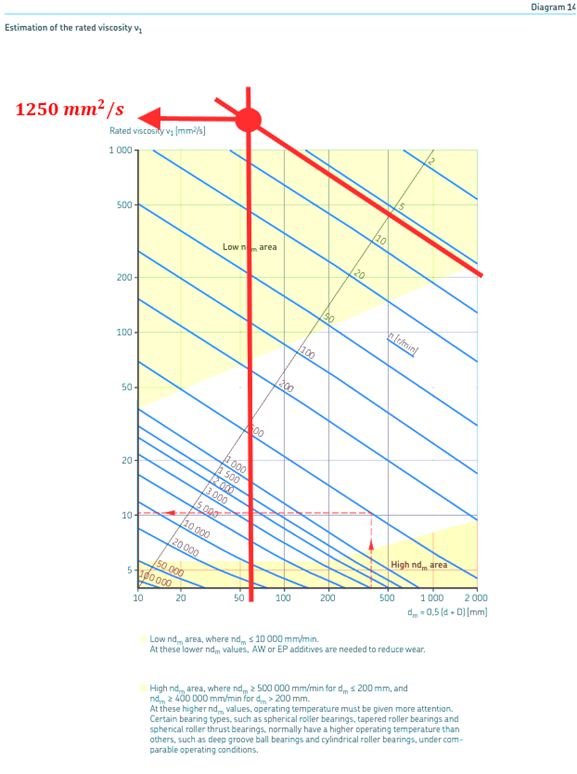
\includegraphics[width=0.5\linewidth]{ratedviscosity.png}
    \caption{Rated viscosity estimation table}
    \label{fig:ratedviscosity}
\end{figure}

The rated viscosity is determined using the mean diameter and angular velocity, as derived from Diagram 14 in the SKF bearing catalog, and is illustrated in the accompanying figure. 

\begin{align}
v_1 = 1250 \, \frac{\text{mm}^2}{\text{s}}
\end{align}
\newpage

Viscosity Value
\begin{figure}[H]
    \centering
    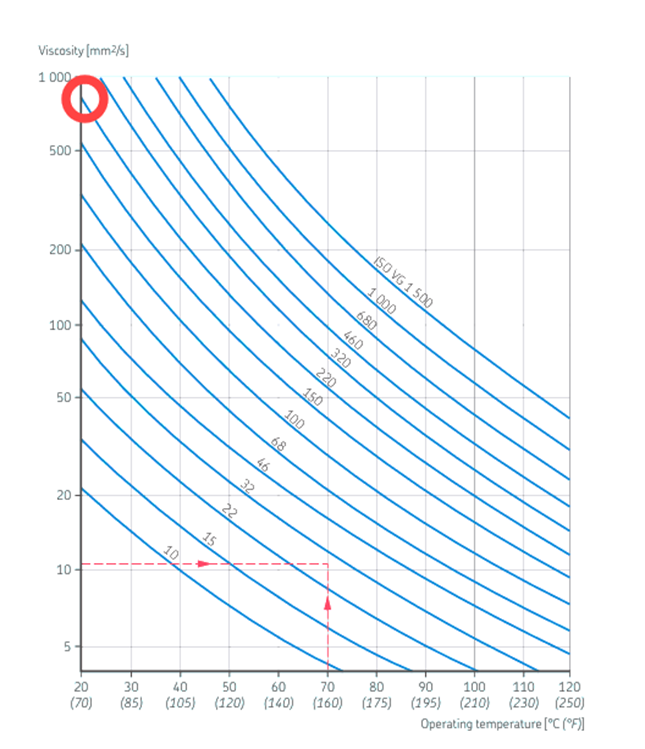
\includegraphics[width=0.6\linewidth]{viscosityvalue.png}
    \caption{Viscosity value table}
    \label{fig:viscosityvalue}
\end{figure}

The lubricant's viscosity is determined based on the operating temperature and the standard lubricant specified in the selected bearing data. The viscosity value is obtained using Diagram 13 of the SKF catalog, as shown below.

\begin{align}
v_{\text{ref}} = 220 \, \frac{\text{mm}^2}{\text{s}}
\end{align}
\begin{align}
T_{\text{operating}} = 20 \, \text{°C}
\end{align}
\begin{align}
v = 1250 \, \frac{\text{mm}^2}{\text{s}}
\end{align}

\newpage

\( a_{\text{SKF}} \) Factor

\begin{figure}[h!]
    \centering
    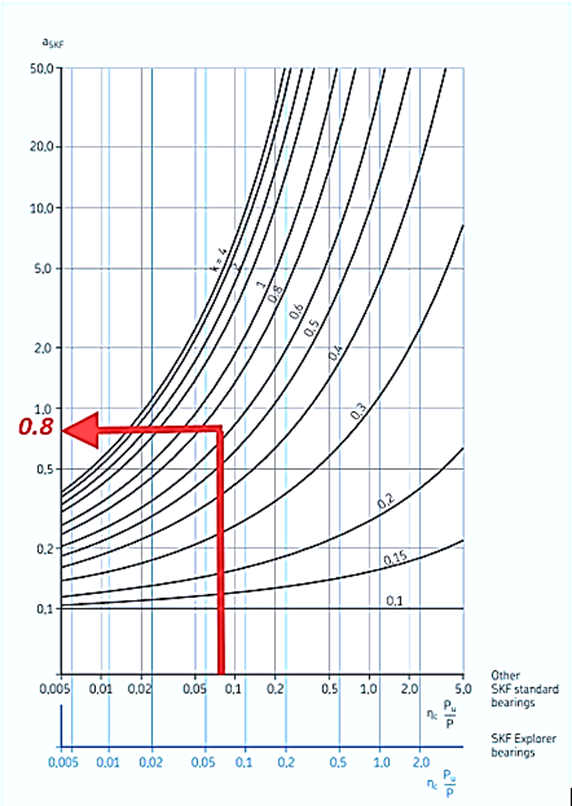
\includegraphics[width=0.6\linewidth]{a_skf.png}
    \caption{a\_skf factor}
    \label{fig:a_skf factor}
\end{figure}


This factor is calculated using the \( \frac{v}{v_1} \) ratio and the contamination factor \( n_c \), which depends on the fatigue load limit \( P_u \). \( P_u \) is provided in the selected bearing data. The relevant equations are provided below. The \( a_{\text{SKF}} \) factor is determined using Diagram 9 from the SKF bearing catalog. The contamination factor \( n_c \) is calculated based on the fatigue load limit \( P_u \), which is typically given in the bearing data sheet. The formula for \( a_{\text{SKF}} \) can be found in Diagram 9 of the SKF bearing catalog, which provides the relationship between various factors and bearing performance under specific conditions.

\begin{align}
\kappa = \frac{v}{v_1} = 0.64
\end{align}
\begin{align}
n_c = \frac{P_u}{P} = 0.08
\end{align}
\begin{align}
a_{\text{SKF}} = 0.8
\end{align}

Rating Life

\( L_{10} \) is the basic rating life (at 90\% reliability).

\( L_{10h} \) is the basic rating life (at 90\% reliability) [operating hours].

\( C \) is the basic dynamic load rating [kN].

\( P \) is the equivalent dynamic bearing load [kN].

\( n \) is the rotational speed [r/min].

\( p \) is the exponent of the life equation:
\[
p = 3 \quad \text{for ball bearings}
\]
\[
p = \frac{10}{3} \quad \text{for roller bearings}
\]

\( L_{nm} \) is the SKF rating life (at \( (100 - n) \)% reliability) [millions of revolutions]:
\begin{align}
L_{nm} = a_1 \cdot a_{\text{SKF}} \cdot L_{10} = a_1 \cdot a_{\text{SKF}} \cdot \left( \frac{C}{P} \right)^p
\end{align}

\begin{figure}[h!]
    \centering
    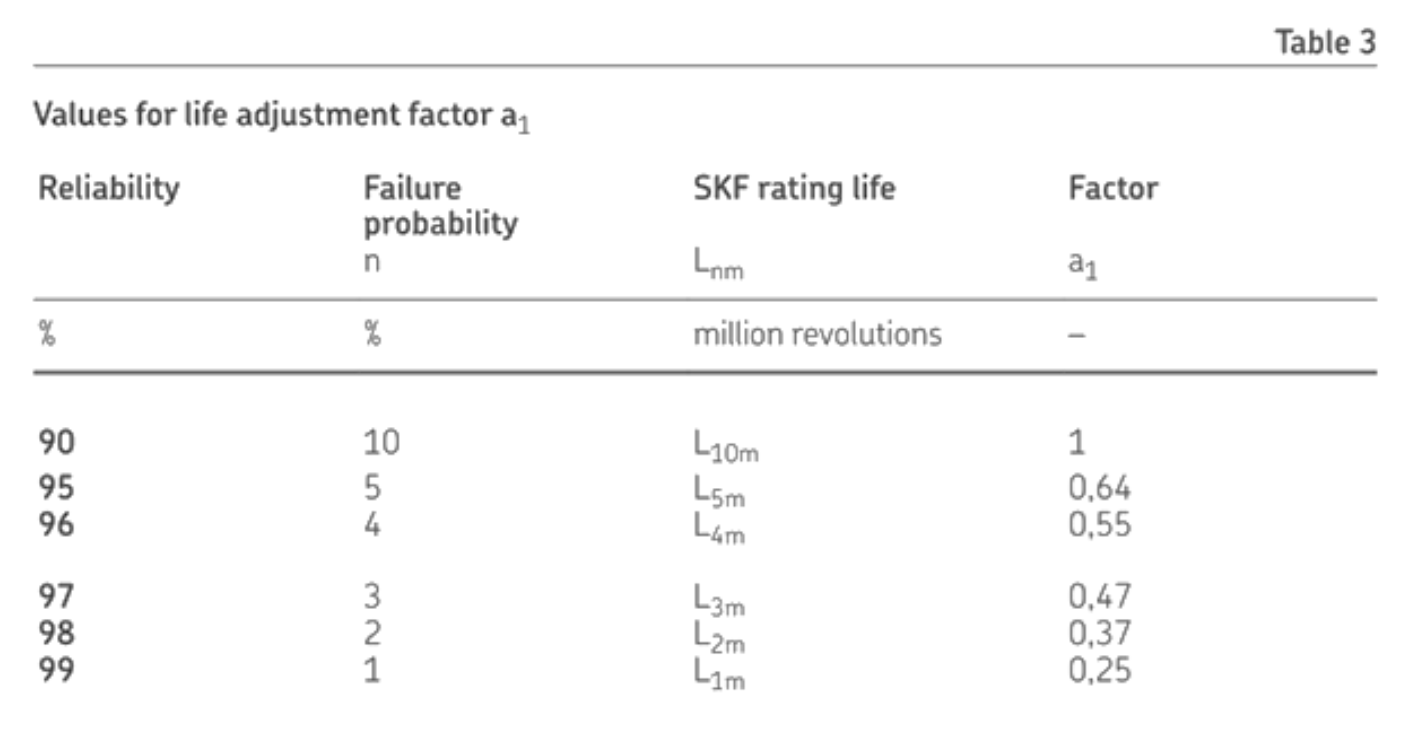
\includegraphics[width=0.5\linewidth]{table3.png}
    \caption{Selection of a1 factor}
    \label{fig:enter-label}
\end{figure}

The SKF rating life in millions of revolutions is:
\begin{align}
L_{nm} = 0.8 \cdot \left( \frac{6.76}{0.2425} \right)^3 = 17329.88 \, [\text{millions of revolutions}]
\end{align}

The basic rating life in operating hours is:
\begin{align}
L_{10h} = \frac{10^6}{60 \cdot n} \cdot L_{10} = 43302977 \, [\text{hours}]
\end{align}
 
The table 6 shows the planned models, analyses, and tests to ensure the system meets the required performance standards. For each part or subsystem, it describes the modeling type (analytical, numerical, or experimental), important design factors, and key methods used.  For instance, numerical modeling will be used to test the feeding motor’s reliability and feed rate, while physical tests will evaluate motor power and ball handling. Siemens NX will design the Maltese wheel geometry, and hand calculations will determine storage capacity. Physical experiments will also optimize the net’s tension. Methods like Design of Experiments (DoE) and safety factor calculations will be applied for various components. 


\begin{table}[H]
\centering
\caption{Decisions based on meeting the performance criteria target (Part 3)}
\scriptsize % Adjust font size if needed (e.g., \small, \scriptsize, \tiny)
\renewcommand{\arraystretch}{1.5}
\setlength{\tabcolsep}{4pt}
\begin{tabular}{|>{\raggedright\arraybackslash}p{4cm}|>{\raggedright\arraybackslash}p{2cm}|>{\raggedright\arraybackslash}p{3cm}|>{\raggedright\arraybackslash}p{7cm}|}
\hline
\textbf{Analytical Modelling / Numerical Modelling / Numerical Experiment / Physical Experiment} & \textbf{Component / Subsystem / Whole System} & \textbf{Design Parameters to be Decided} & \textbf{Explanation} \\ \hline
Numerical Modelling & Feeding Motor & Motor Type, Feed Frequency & Feed rate calculations for transferring 25–80 balls/min. A stepper motor-based feeding system (Maltese wheel) will be numerically tested for feed frequency and reliability. DoE (Design of Experiments) will analyze feed rate efficiency. \\ \hline
Physical Experiment & Feeding Motor & Motor Power, Ball Handling & Ball feeding will be tested using physical prototypes. Multiple trials will confirm feed consistency under real-world loads. \\ \hline
Numerical Modelling & Feeding Motor Mounting & Mounting Method, Fasteners & Test motor fixation methods (bolts, clamps) for rigidity and vibration resistance under operation. \\ \hline
Analytical Modelling & Maltese Wheel & Maltese Wheel Geometry & The lengths of the slots and the base dimensions are designed using Siemens NX, ensuring a proper fit for the balls based on their dimensions. \\ \hline
Numerical Modelling + Physical Experiment & Storage & Capacity of Reservoir & A capacity analysis is conducted by hand considering the sizes of the balls. \\ \hline
Numerical Modelling & Clamp Bolt & Safety Factor of Clamp & It is assumed that all the bolts take equal load. The friction factor is taken as 0.2. A multiplication factor of 0.9 is added to ensure that the bolts do not reach their ultimate tensile strength. A safety factor is calculated even for brass. \\ \hline
Physical Experiment & Net & Net Specifications & The physical experiment can be done to find the optimum tension of the net to obtain maximum catching feature. \\ \hline
\end{tabular}
\label{tab:performance_criteria}
\end{table}

\subsubsection{Feeding Mechanism Calculations}

\textbf{Maltese Wheel Free Body Diagram \& Dynamic Analysis:}


\begin{figure}[h!]
    \centering
    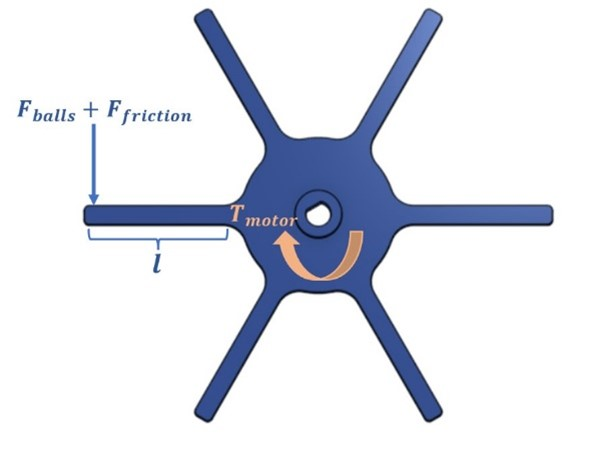
\includegraphics[width=0.5\textwidth]{Figures/maltese wheel fbd.jpg} 
    \caption{Free-body diagram of Maltese wheel}
    \label{fig:fbd maltese} 
\end{figure}


The free-body diagram of the Maltese Wheel is presented above. In the force analysis, the weight of the balls and the frictional forces between the pipe and the balls are taken into account. The subsequent calculations will be derived based on this free-body diagram.
Additionally, a stepper motor is employed to rotate the Maltese Wheel. The subsequent calculations incorporate certain specifications of the motor, which are detailed in Table \ref{stepper}.

\begin{table}[h!]
    \centering
    \caption{Specifications of the 17HS3401S Motor}
    \scriptsize
    \label{stepper}
    \begin{tabular}{>{\raggedright\arraybackslash}m{5cm} >{\raggedleft\arraybackslash}m{3cm}}
        \multicolumn{2}{c}{\textbf{17HS3401S Motor Specification}} \\ \hline
        \textbf{Step Angle (deg)} & 1.8 \\
        \textbf{No of Phases} & 2 \\
        \textbf{Holding Torque (N$\cdot$m)} & 0.28 \\
        \textbf{Rated Current (A)} & 1.3 \\
        \textbf{Rated Voltage (V)} & 3.4 \\
        \textbf{Max. Slewing Rate (pps)} & $\geq$2000 \\
        \textbf{Max. Starting Rate (pps)} & $\geq$1400 \\
    \end{tabular}
    \label{tab:motor_specs}
\end{table}


Additionally, the notations and corresponding values to be used in the subsequent calculations are presented below.


\begin{table}[h!]
\centering
\label{tab:system_parameters}
\begin{tabular}{ll} 
Mass of each ball (2.7 grams)  & $m$  \\ 
Arm length of Maltese wheel (30 mm) & $l$ \\ 
Number of balls in the pipe & $n$ \\ 
Friction coefficient between the balls and the pipe section  & $\mu$  \\ 
\end{tabular}
\end{table}



The friction coefficient between the balls and the pipe is conservatively selected as 0.5 to ensure safety in the design. Typically, friction coefficients for PVC or plastic pipes range from 0.2 to 0.4. Additionally, surface finish plays a critical role in determining frictional performance. Therefore, during manufacturing, careful attention will be given to achieving a high-quality surface finish on the interior of the pipe to optimize frictional characteristics.

\begin{align}
F_g = m \cdot g = 0.0027 \, \text{kg} \cdot 9.81 \, \text{m/s}^2 = 0.0265 \, \text{N}
\end{align}
\begin{align}
F_{\text{friction}} = \mu \cdot F_g = 0.5 \cdot 0.0265 \, \text{N} = 0.01325 \, \text{N}
\end{align}
\begin{align}
n \cdot (F_g + F_{\text{friction}}) \cdot l = T_{\text{motor}}
\end{align}
\begin{align}
n \cdot (0.0265 \, \text{N} + 0.01325 \, \text{N}) \cdot 0.03 \, \text{m} = 0.28 \, \text{Nm}
\end{align}
\begin{align}
n = 234 \, \text{balls}
\end{align}

In the pipe section, the stepper motor attached to the Maltese wheel is capable of handling the combined weight and friction of up to 234 balls.
 In our design, the pipe section is intended to hold a maximum of 20 balls. Therefore, even under the worst-case conditions, no failure is anticipated.
 
\textbf{Maltese Wheel Maximum Attainable Frequency Calculation:}

Frequency, in the context of this project, refers to the number of balls fed per second. To ensure compliance with the design criterion, a series of calculations must be performed. First, the rotational speed of the stepper motor, as defined by its specifications, must be determined, as it directly influences the operation of the Maltese Wheel. Next, the time required to feed a single ball can be calculated. Finally, the total feeding frequency can be derived, ensuring the design criterion is met.


\begin{equation}
\text{Steps per revolution} = \frac{360^\circ}{1.8^\circ} = 200 \, \text{steps/rev}
\end{equation}

\begin{equation}
\text{Motor RPS} = \frac{\text{Pull-out frequency (pps)}}{\text{Steps per revolution}} = \frac{2000 \, \text{pps}}{200 \, \text{steps/rev}} = 10 \, \text{rps}
\end{equation}

\begin{equation}
\text{Output Shaft RPS} = \text{Motor RPS} \cdot \text{Reduction ratio}
\end{equation}

\begin{equation}
\text{Output RPS} = 10 \, \text{rps}
\end{equation}

\begin{equation}
\text{6-slot Maltese wheel completes one full cycle in} \quad \frac{1}{6} \, \text{of a revolution.}\notag
\end{equation}

\begin{equation}
t_{\text{cycle}} = \frac{1}{\text{Output RPS} \cdot \text{Number of slots}} = \frac{1}{10 \cdot 6} = 0.017 \, \text{seconds}
\end{equation}

\begin{equation}
f_{\text{max}} = \frac{1}{t_{\text{cycle}}} = \frac{1}{0.017 \, \text{seconds}} = 58.8 \, \text{balls/second}
\end{equation}

\begin{equation}
80 \, \text{balls/minute} = \frac{80}{60} \, \text{balls/second} = 1.33 \, \text{balls/second}
\end{equation}

Based on the preceding calculations, the criterion for maximum feeding frequency is achievable. Theoretical analysis indicates that the maximum attainable frequency, governed by the stepper motor's specifications, is 58 balls per second. In contrast, the design criterion specifies a requirement of 1.33 balls per second. 

\subsubsection{Storage Capacity Calculations}

A storage system utilizing an inclined groove has been designed, and its dimensions are provided below the figure. Based on these dimensions and the standard ball size, a capacity calculation has been conducted.

\begin{figure}[h!]
    \centering
    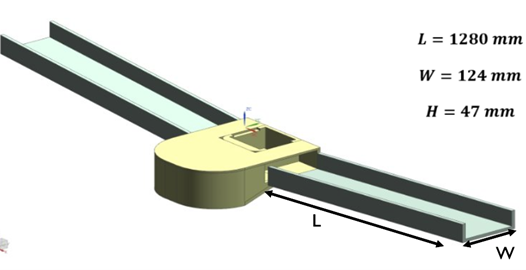
\includegraphics[width=0.35\textwidth]{Figures/storage capacity.png} 
    \caption{Model of inclined groove}
    \label{fig:storage} 
\end{figure}

\begin{equation}
\label{eq68}
\text{Capacity} = \frac{L}{\text{Ball diameter}} \cdot \frac{W}{\text{Ball diameter}} \cdot \frac{H}{\text{Ball diameter}}
\end{equation}

A standard table tennis ball has a diameter of 40 mm.A standard table tennis ball has a diameter of 40 mm. Capacity of the designed groove can be estimated roughly by using Equation \ref{eq68}
Each term is rounded to the lowest integer before multiplication to ensure a meaningful result in terms of ball numbers.
\begin{equation}
\text{Capacity} = \frac{1280 \, \text{mm}}{40 \, \text{mm}} \cdot \frac{124 \, \text{mm}}{40 \, \text{mm}} \cdot \frac{47 \, \text{mm}}{40 \, \text{mm}} = 32 \cdot 3 \cdot 1 = 96 \, \text{balls}
\end{equation}

As a result, the designed groove can store a minimum of 96 balls before launching.

\subsection{Decisions based on avoiding all potential failures (component or system level)}

In this section, the decisions based on avoiding all potential failure modes (component or system level) are presented. The possible modes of possible critical failure modes are jamming of the Maltese wheel, explosion of the disk rubber, squeezing of the balls at the launching mechanism, vibration of the frame, buckling of the pipe, failure (bending) of the clamp. 

\begin{table}[H]
\centering
\caption{Failure Scenarios and Related Design Parameters}
\scriptsize % Adjust font size if needed (e.g., \small, \scriptsize, \tiny)
\renewcommand{\arraystretch}{1.5}
\setlength{\tabcolsep}{4pt}
\begin{tabular}{|>{\raggedright\arraybackslash}p{2cm}|>{\raggedright\arraybackslash}p{3cm}|>{\raggedright\arraybackslash}p{2cm}|>{\raggedright\arraybackslash}p{3cm}|>{\raggedright\arraybackslash}p{5cm}|}
\hline
\textbf{Failure Scenario} & \textbf{Analytical Modelling / Numerical Modelling / Numerical Experiment / Physical Experiment} & \textbf{Component / Subsystem / Whole system} & \textbf{Design Parameters to be Decided} & \textbf{Explanation} \\ \hline
 Jamming & Physical Experiment and Analytical Modelling & Maltese Wheel & Maltese Wheel Arm Number and Alignment & Physical experiments will test different number of arms (e.g., 4, 6, or 8 arms) and their alignment angles to optimize ball feeding performance while minimizing jamming. A prototype will be built, and experiments will monitor ball flow continuity. \\ \hline
 Exploding & Physical Experiment & Disk Rubber   & Disk Rubber Material  & Physical experiments will evaluate various rubber materials for the launching disks. Testing will focus on grip performance, material wear, and deformation under high rotational speeds (up to 9550–11460 RPM) \\ \hline
 Squeezing of balls & Physical Experiment &  Launching Mechanism & Design of Launcher & Mounting positions can be adjusted physically to find the optimum ball press \\ \hline
 Vibration & Physical Experiment & Frame & Rigidity of frame & Test rigidity and measure deflection under load.
Compare materials.  
 \\ \hline
 Bending & Numerical Modelling & Clamp & Worst Case Stresses & Assuming the lower portion of the clamp is not securely connected will be analyzed using Finite Element Analysis (FEA) using ANSYS. \\ \hline
 Buckling & Numerical Modelling & Neck & Buckling of Neck & The end conditions are taken as one end fixed and one end free. For a conservative approach, the elastic modulus of pipe material is taken as the lowest value from the interval. The pipe is taken as an intermediate-length column and critical buckling force is computed. \\ \hline
\end{tabular}
\label{tab:empty_table}
\end{table}

\subsubsection{Clamping force and Factor of Safety calculations to determine the number of bolts }

Initially, a clamp with 4 bolts with 5 mm diameter is used to fix the device to the table.
To determine the clamping force, the torque of the clamps should be calculated initially. The weight of the ball pitcher machine is 4.5 kg. The horizontal dimension of the machine is 130 mm, as well. Assuming that the ball pitcher is uniform (its center of mass is in the middle)

\begin{align}
T = \frac{F \cdot d}{2} = \frac{m \cdot g \cdot d}{2} = 4.5 \, \text{kg} \cdot 9.81 \, \frac{\text{m}}{\text{s}^2} \cdot 65 \times 10^{-3} \, \text{m} = 2.87 \, \text{N} \cdot \text{m}
\end{align}

As mentioned, bolt diameter (d) is taken as 5 mm, and the friction coefficient K is 0.2.
Total clamping force is calculated by the formulation below:

The total force \( F \) is given by:
\begin{align}
F = \frac{T}{K \cdot d} = \frac{2.87 \, \text{N} \cdot \text{m}}{0.2 \cdot 5 \times 10^{-3} \, \text{m}} = 2870 \, \text{N} \quad (\text{for 4 bolts})
\end{align}

Assuming all 4 bolts take equal amounts of load:
\begin{align}
F_{\text{each}} = \frac{2870 \, \text{N}}{4} = 717.5 \, \text{N}
\end{align}

Determination of Factor of Safety

The factor of safety (FoS) can be calculated using the equation:
\begin{align}
\text{FoS} = \frac{A \cdot 0.9 \cdot \text{UTS}}{F_{\text{each}}}
\end{align}
where:
- \( A \) represents the cross-sectional area of the bolt,
- UTS is the ultimate tensile strength of the bolt material,
- \( F_{\text{each}} \) is the load per bolt as calculated earlier.

The cross-sectional area of the bolt is given by:
\begin{align}
A = \frac{\pi d^2}{4} = \frac{\pi \left( 5 \times 10^{-3} \, \text{m} \right)^2}{4} = 1.963 \times 10^{-5} \, \text{m}^2
\end{align}

The multiplication factor of \( 0.9 \) is used to ensure that the bolt does not reach its ultimate tensile strength, leaving a safety margin.

The ultimate tensile strength (UTS) values for the material are as follows:
- For carbon steel, \( \text{UTS} \approx 800 \, \text{MPa} \).
- For a counterpart made of brass, \( \text{UTS} \approx 100 - 200 \, \text{MPa} \). To be conservative, we use \( \text{UTS} = 100 \, \text{MPa} \).

The factor of safety is calculated under these two conditions:

\textbf{If carbon steel is used:}
\begin{align}
\text{FoS} = \frac{1.963 \times 10^{-5} \, \text{m}^2 \cdot 0.9 \cdot 800 \, \text{MPa}}{717.5 \, \text{N}} = 19.69
\end{align}

\textbf{If a counterpart (brass) is used:}
\begin{align}
\text{FoS} = \frac{1.963 \times 10^{-5} \, \text{m}^2 \cdot 0.9 \cdot 100 \, \text{MPa}}{717.5 \, \text{N}} = 2.46
\end{align}

Even if a counterpart (brass) is used, the clamps are still safe. However, we also need to consider the case when only 2 bolts are used.

\textbf{If 2 bolts are used:}
\begin{align}
F_{\text{each}} = \frac{2870 \, \text{N}}{2} = 1435 \, \text{N}
\end{align}

\textbf{If carbon steel is used:}
\begin{align}
\text{FoS} = \frac{1.963 \times 10^{-5} \, \text{m}^2 \cdot 0.9 \cdot 800 \, \text{MPa}}{1435 \, \text{N}} = 9.85
\end{align}

\textbf{If a counterpart (brass) is used:}
\begin{align}
\text{FoS} = \frac{1.963 \times 10^{-5} \, \text{m}^2 \cdot 0.9 \cdot 100 \, \text{MPa}}{1435 \, \text{N}} = 1.231 \quad (\text{not high enough to use})
\end{align}

Since the factor of safety for 2 bolts is not high enough, it was decided to use 4 bolts. Based on these calculations, M5 bolts will be used to ensure an acceptable factor of safety.



\subsubsection{Buckling condition calculations of the vertical pipe section}

The vertical section of the pipe is inspected if there could be a failure due to buckling.
Fc is the critical load to make buckling, E is the elastic modulus of the pipe material (PVC), I is the smallest moment of inertia of the pipe section, C is a multiplication factor depending on the begin and end conditions. Finally, L is the length of the column. 
The outer diameter (D) of the pipe is 50 mm and inner diameter (d) is 44 mm. The length of the pipe is 130 mm. The elastic modulus of PVC ranges between 2.8 to 4.1 GPa. For a conservative approach, smallest value is taken. For one end is fixed and one end is free condition, C is taken as 0.25.
\begin{figure}[h]
    \centering
    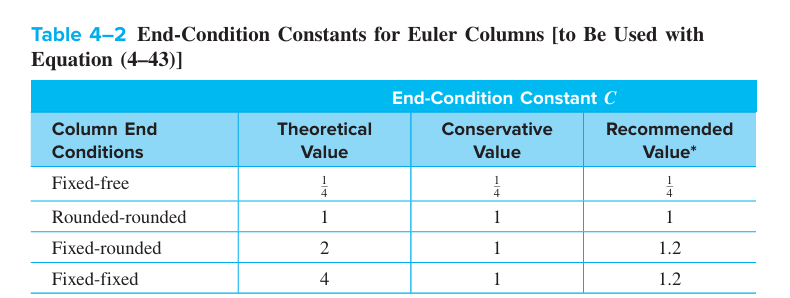
\includegraphics[width=0.7\textwidth]{Figures/buckling conditions.png}
    \caption{Buckling condition constants}
    \label{fig:buckling}
\end{figure}

The critical force \( F_{\text{cr}} \) per unit area \( A \) is calculated by the following equation:
\begin{align}
\frac{F_{\text{cr}}}{A} = S_y - \left( \frac{S_y}{2\pi} \right)^2 \cdot \frac{1}{C \cdot E} \cdot \left( \frac{l}{k} \right)^2
\end{align}
where:
- \( S_y \) is the yield strength of the material,
- \( \frac{l}{k} \) is the slenderness ratio, which is determined by:
\begin{align}
\frac{l}{k} = \sqrt{\frac{2 \pi^2 C E}{S_y}}
\end{align}

The yield strength of PVC is taken as \( S_y = 50 \, \text{MPa} \), and the slenderness ratio is calculated as:
\begin{align}
\frac{l}{k} = \sqrt{\frac{2 \pi^2 \cdot 0.25 \cdot (2.8 \, \text{GPa})}{50 \, \text{MPa}}} = 16.62
\end{align}

The critical force per unit area is then calculated:
\begin{align}
\frac{F_{\text{cr}}}{A} = 50 \, \text{MPa} - \left( \frac{50 \, \text{MPa}}{2\pi} \right)^2 \cdot \frac{1}{0.25 \cdot 2.8 \, \text{GPa}} \cdot 16.62^2 = 25 \, \text{MPa}
\end{align}

The critical force is calculated by:
\begin{align}
F_{\text{cr}} = 25 \, \text{MPa} \cdot \frac{\pi (D^2 - d^2)}{4} = 11074 \, \text{N}
\end{align}


Since the maximum force acting on the pipe is:
\begin{align}
F_{\text{max}} = 2 \, \text{kg} \cdot 9.81 \, \frac{\text{m}}{\text{s}^2} = 19.62 \, \text{N}
\end{align}
which is much smaller than the critical force, buckling is not a concern in this case.

\subsubsection{Bolt Calculations}
\begin{figure}[h]
    \centering
    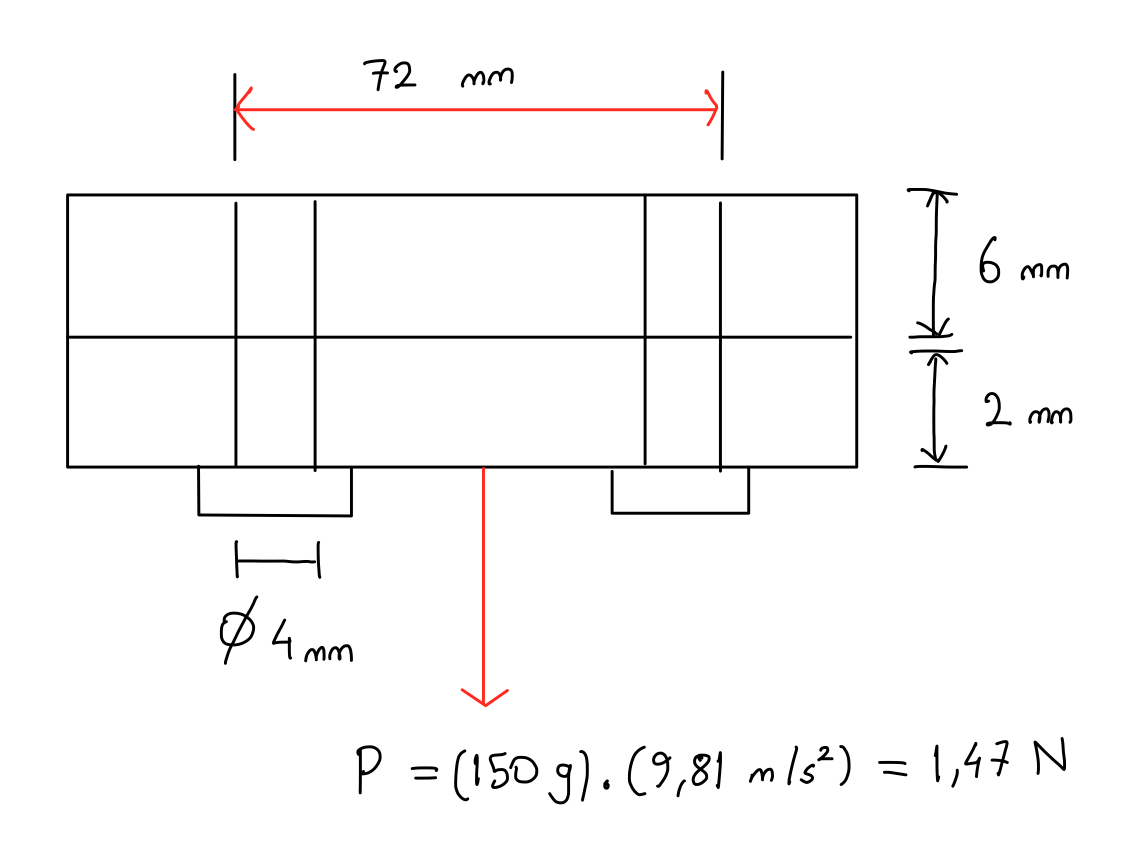
\includegraphics[width=0.5\textwidth]{Figures/bolts.jpg}
    \caption{FBD of bolt}
    \label{fig:bolt}
\end{figure}

For static loading and nonpermanent connections, the force on each bolt \( F_i \) is given by:
\begin{align}
F_i = 0.75 \cdot F_p
\end{align}
where \( F_p \) is the load based on the yield strength of the material. The force \( F_p \) is calculated as:
\begin{align}
F_p = S_p \cdot A_t
\end{align}
where:
- \( S_p \) is the permissible yield strength of the material, and
- \( A_t \) is the cross-sectional area of the bolt.

The permissible yield strength \( S_p \) is calculated as:
\begin{align}
S_p = 0.85 \cdot S_y
\end{align}
where the yield strength \( S_y \) of brass is taken as \( 70 \, \text{MPa} \) for the safest approach:
\begin{align}
S_p = 0.85 \cdot 70 \, \text{MPa} = 59.5 \, \text{MPa}
\end{align}

The cross-sectional area \( A_t \) for an M4 metric bolt is \( 8.78 \, \text{mm}^2 \), so the force \( F_p \) is:
\begin{align}
F_p = 59.5 \, \text{MPa} \cdot 8.78 \, \text{mm}^2 = 522.4 \, \text{N}
\end{align}
Thus, the force \( F_i \) on each bolt is:
\begin{align}
F_i = 522.4 \, \text{N} \cdot 0.75 = 391.8 \, \text{N}
\end{align}

The elastic modulus of brass is taken as \( E = 90 \, \text{GPa} \) (minimum), and the stiffness factor \( k_t \) for the bolt is:
\begin{align}
k_t = \frac{A_t \cdot E}{l_t} = \frac{8.78 \, \text{mm}^2 \cdot 90 \, \text{GPa}}{8 \, \text{mm}} = 98.78 \, \text{MN/m} = k_b
\end{align}
where \( k_b \) represents the bolt's stiffness.

The member stiffness of ABS (Acrylonitrile Butadiene Styrene) is given by:
\begin{align}
k_m = 0.5774 \cdot \pi \cdot E \cdot d \left/ \left( 2 \cdot \ln \left( \frac{5 \cdot (0.5774 \cdot l + 0.5 \cdot d)}{0.5774 \cdot l + 2.5 \cdot d} \right) \right) \right.
\end{align}
Substituting the given values for the elastic modulus of ABS (\( E = 2 \, \text{GPa} \)) and the diameter \( d \), and the length \( l \), the member stiffness \( k_m \) is:
\begin{align}
k_m = 8.881 \, \text{MN/m}
\end{align}

The load share coefficient \( C \) is calculated by:
\begin{align}
C = \frac{k_b}{k_b + k_m} = \frac{98.78}{98.78 + 8.881} = 0.918
\end{align}
This value indicates that most of the load is taken by the bolts.

The stress \( \sigma_i \) on each bolt is given by:
\begin{align}
\sigma_i = \frac{F_i}{A_t} = \frac{391.8 \, \text{N}}{8.78 \, \text{mm}^2} = 44.62 \, \text{MPa}
\end{align}

The torque \( T \) on the bolt is calculated as:
\begin{align}
T = K \cdot F_i \cdot d = 0.15 \cdot 391.8 \, \text{N} \cdot 4 \, \text{mm} = 235 \, \text{N} \cdot \text{m}   
\end{align}

The polar moment of inertia \( J \) of the bolt is:
\begin{align}
J = \frac{\pi \cdot (4 \, \text{mm})^4}{32} = 25.1 \, \text{mm}^4
\end{align}

The shear stress \( \tau \) is given by:
\begin{align}
\tau = \frac{T \cdot r}{J} = \frac{235 \, \text{N} \cdot \text{m} \cdot (2 \, \text{mm})}{25.1 \, \text{mm}^4} = 18.72 \, \text{MPa}
\end{align}

The principal stresses \( \sigma_1 \) and \( \sigma_2 \) are calculated as:
\begin{align}
\sigma_1, \sigma_2 = \frac{44.62 \, \text{MPa}}{2} \pm \sqrt{\left( \frac{44.62 \, \text{MPa}}{2} \right)^2 + (43.23 \, \text{MPa})^2}
\end{align}
The results are:
\begin{align}
\sigma_1 = 71 \, \text{MPa}, \quad \sigma_2 = -26 \, \text{MPa}
\end{align}

The case \( \sigma_1 > 0 > \sigma_2 \) applies to:
\begin{align}
\sigma_1 - \sigma_2 = \frac{S_y}{n}
\end{align}
Using the Maximum Shear Stress Theory, the safety factor \( n \) is calculated as:
\begin{align}
n = \frac{70 \, \text{MPa}}{71 \, \text{MPa} + 26 \, \text{MPa}} = 0.72
\end{align}


\subsubsection{Failure}

The minimum yield strength is:
\begin{align}
S_y = 71 \, \text{MPa} + 26 \, \text{MPa} = 97 \, \text{MPa}
\end{align}
Brass with a minimum yield strength of \( 200 \, \text{MPa} \) would be sufficient. However, since metric bolts typically have no standard load-carrying capacities on the market (even during tightening), process is to be continued with stainless steel, which has a minimum yield strength of \( S_y = 200 \, \text{MPa} \).

The elastic modulus for stainless steel is:
\begin{align}
E = 200 \, \text{GPa}
\end{align}
The stiffness for the bolt is:
\begin{align}
k_t = \frac{A_t \cdot E}{l_t} = \frac{8.78 \, \text{mm}^2 \cdot 200 \, \text{GPa}}{8 \, \text{mm}} = 219.5 \, \text{MN/m} = k_b
\end{align}

The load share coefficient \( C \) is calculated by:
\begin{align}
C = \frac{k_b}{k_b + k_m} = \frac{219.5}{219.5 + 8.881} = 0.961
\end{align}

The load per bolt is:
\begin{align}
P = P_b + P_m
\end{align}
\begin{align}
P_b = C \cdot P = 0.961 \cdot 0.736 \, \text{N} = 0.707 \, \text{N}
\end{align}

The total force on the bolt is:
\begin{align}
F_b = C \cdot P + F_i = 0.707 \, \text{N} + 391.8 \, \text{N} = 392 \, \text{N}
\end{align}

The stress on the bolt is:
\begin{align}
\sigma_b = \frac{392 \, \text{N}}{8.82 \, \text{mm}^2} = 44.4 \, \text{MPa}
\end{align}

The safety factor for the bolt is:
\begin{align}
n_b = \frac{S_p}{\sigma_b} = \frac{0.85 \cdot 200 \, \text{MPa}}{44.4 \, \text{MPa}} = 3.8
\end{align}

For the separation case, the separation factor is:
\begin{align}
n_o = \frac{391.8 \, \text{N}}{0.707 \cdot (1 - 0.961)} = 14210
\end{align}
Since the separation factor is very high, separation is not possible.

Finally, for bolts, the distance between them should be at least \( 1D \) from the corners. This rule is obeyed in the design.

\subsubsection{Curved Member Analysis for the Clamp }
\begin{figure}[h]
    \centering
    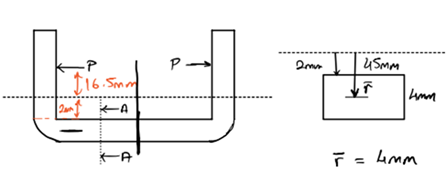
\includegraphics[width=0.7\textwidth]{Figures/curvedmember.png}
    \caption{FBD of the clamp connection}
    \label{fig:curvedmember}
\end{figure}

The centroid and cross-sectional area of the material are calculated as:
\begin{align}
\overline{r} = 4 \, \text{mm}, \quad A = (45 \, \text{mm}) \times (4 \, \text{mm}) = 180 \, \text{mm}^2
\end{align}

For ABS material, the yield strength is given as:
\begin{align}
\sigma_y = 45 \, \text{MPa}
\end{align}

Considering the curved section as the most critical cross-section, the radius of curvature \( r_n \) is calculated by:
\begin{align}
r_n = \frac{A}{\int_{2 \, \text{mm}}^{4 \, \text{mm}} \frac{dr}{r}} = \frac{180 \, \text{mm}^2}{45 \ln \left( \frac{4}{2} \right)} = 5.771 \, \text{mm}
\end{align}

Next, the bending moment \( M \) is calculated as:
\begin{align}
M = P(4 \, \text{mm} + 16.5 \, \text{mm}) = 20.5 \, \text{mm} \cdot P
\end{align}

The stress in the material is then expressed as:
\begin{align}
\sigma = \frac{M \cdot c_i}{A \cdot e \cdot r_i} + \frac{P}{A}
\end{align}

Where:
\begin{align}
e = \overline{r} - r_n = 4 \, \text{mm} - 5.771 \, \text{mm} = -1.771 \, \text{mm}
\end{align}
\begin{align}
c_i = r_n - r_i = 5.771 \, \text{mm} - 2 \, \text{mm} = 3.771 \, \text{mm}
\end{align}

For the allowable stress, we have:
\begin{align}
45 \, \text{MPa} = (20.5 \, \text{mm}) \cdot P \cdot \frac{3.771 \, \text{mm}}{180 \, \text{mm}^2 \cdot (-1.771 \, \text{mm}^2) \cdot (2 \, \text{mm})} + \frac{P}{180 \, \text{mm}^2}
\end{align}

The allowable force \( P_{all} \) is:
\begin{align}
P_{all} = 389 \, \text{N}
\end{align}

Assuming the clamp is carrying a load of 4.5 kg, we calculate the force as:
\begin{align}
P = 4.5 \, \text{kg} \cdot 9.81 \, \text{m/s}^2 = 44.15 \, \text{N} \ll 389 \, \text{N}
\end{align}

Thus, the load is much smaller than the allowable stress, confirming that the clamp is safe under the given conditions.

\begin{table}[h!]
\centering
\caption{List of final values of design decisions and parameters}
\scriptsize
\begin{tabular}{|l|l|}
\hline
\textbf{Relevant Component/Subsystem}       & \textbf{Final Results for Design Decision or Parameter} \\ \hline
Launcher Motor                              & BLDC EMAX MT2204 + ESC XW-30A                           \\ \hline
Launcher Motor Mounting                     & M3                                                     \\ \hline
Disk Dimensions                             & 62 mm diameter                                         \\ \hline
Disk Cover Material                         & Plates Band                                            \\ \hline
Motor of Yaw Angle                          & Tower Pro MG996 R                                      \\ \hline
Motor of Pitch Angle                        & Tower Pro MG90                                         \\ \hline
Yaw Angle Gear Dimensions                   & Module 1.5, 55 and 25 tooth number                     \\ \hline
Pitch Angle Gear Dimensions                 & Module 1, 65 and 17 tooth number                       \\ \hline
Feeding Motor                               & NEMA 17 Stepper                                       \\ \hline
Feeding Motor Mounting                      & M4                                                     \\ \hline
Maltese Wheel Arm Length                    & 30 mm                                                  \\ \hline
Maltese Wheel Arm Number                    & 6                                                      \\ \hline
Capacity of Reservoir                       & 96 balls in Reservoir + 12 balls in machine            \\ \hline
Bearing Dimensions (Yaw Angle)             & SKF 6810 - D:65 mm d:50 mm B:7 mm                      \\ \hline
Clamp                                       & G Clamp                                                \\ \hline
Frame                                       & Sigma Profile                                          \\ \hline
Total Bolts of Clamp                        & 4                                                      \\ \hline
Bolt Type of Clamp                          & M5                                                     \\ \hline
\end{tabular}
\end{table}


\section{Analysis Results}

To determine the stress distributions and inspect any potential failure of the system, most critical parts are analyzed and the results of these analyses are demonstrated below. This procedure is implemented for feeding holder part, Maltese wheel, the bottom part of the main body, pipe elbow and pitch angle horizontal part. It is crucial and helpful to have an idea about the parts/sections that are failure-prone. Foreseeing the parts that have tendency to fail enables one to fix the issues beforehand, which is beneficial in terms of time and cost. Also, safety of the customer is taken care of by identifying these potential failures.


\begin{figure}[H]
    \centering
    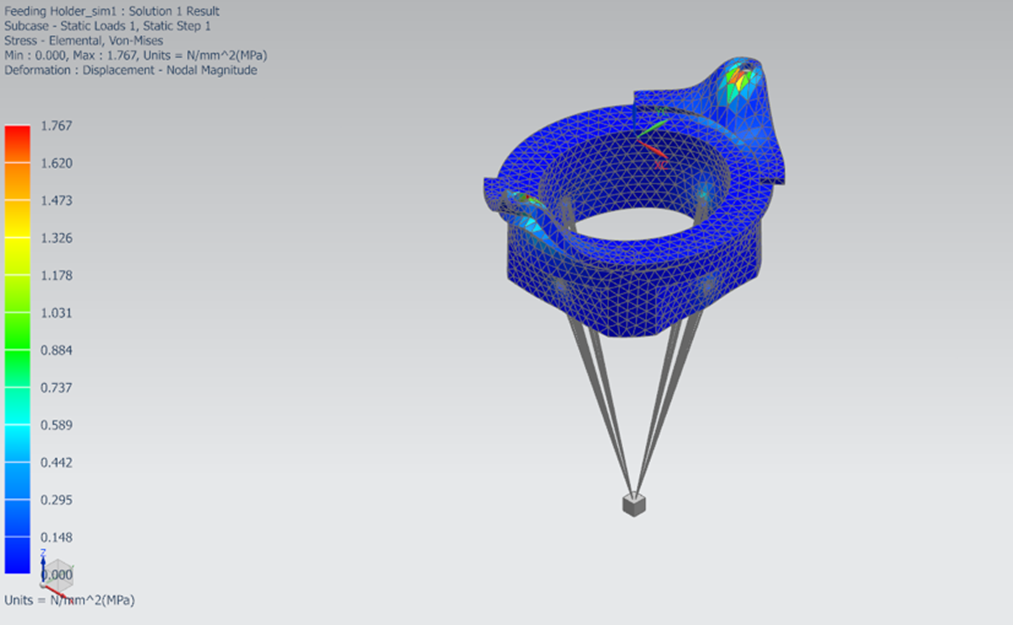
\includegraphics[width=0.65\linewidth]{feedingholderfinal.png}
    \caption{Analysis result of feeding holder}
    \label{fig:feedingholderanalysis}
\end{figure}

Initially, a stress analysis is completed for the feeding holder part. As it can be seen, the most critical sections are determined as the holed upward sections, as expected. In other words, 1.767 MPa is the maximum amount of stress in the part. Except these holed sections, there are not any stress concentrations. 
An analysis scenario has been created considering the loads and stresses that this part will be exposed to. According to this scenario, a point mass was created.  The purpose of this point mass is to simulate the weight created by the downstream feeding mechanism. The point load is connected to the bolt connection points of the part with one-dimensional 1D connection called RB2. Fixed constraint was applied to the part where the clamp would be mounted. and finally a gravitational acceleration of 1.5 g was applied in the downward direction. Under these conditions, the analysis results were observed and no possible problems were found.


\begin{figure}[H]
    \centering
    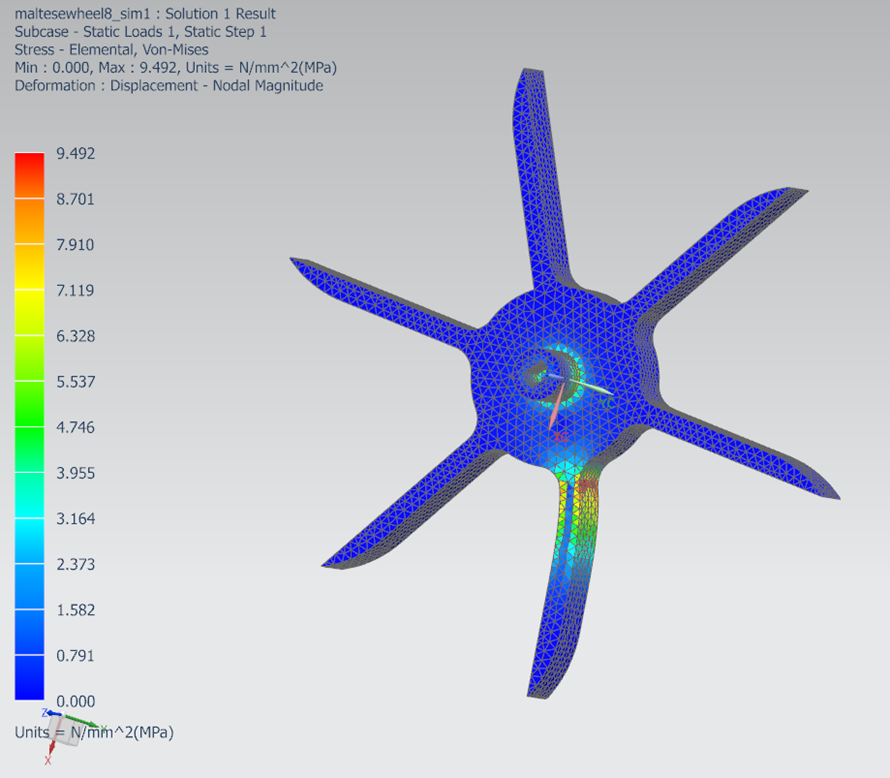
\includegraphics[width=0.5\linewidth]{malteseanalysisfinal.png}
    \caption{Analysis result of Maltese wheel}
    \label{fig:malteseanalysisfinal}
\end{figure}

Then, the elemental stress test is completed for the Maltese wheel in order to see is any section or part of the Maltese wheel has tendency to fail under excessive stresses. 
The thrust required to feed the balls will be transmitted through this part. Considering these conditions, the normal forces required to push the ball to the area where the balls will contact are also added on the application. The part is applied fixed constraint from the motor connection area in the center. Also, ABS material is used for this part because of its high ultimate tensile strength.

\begin{figure}[H]
    \centering
    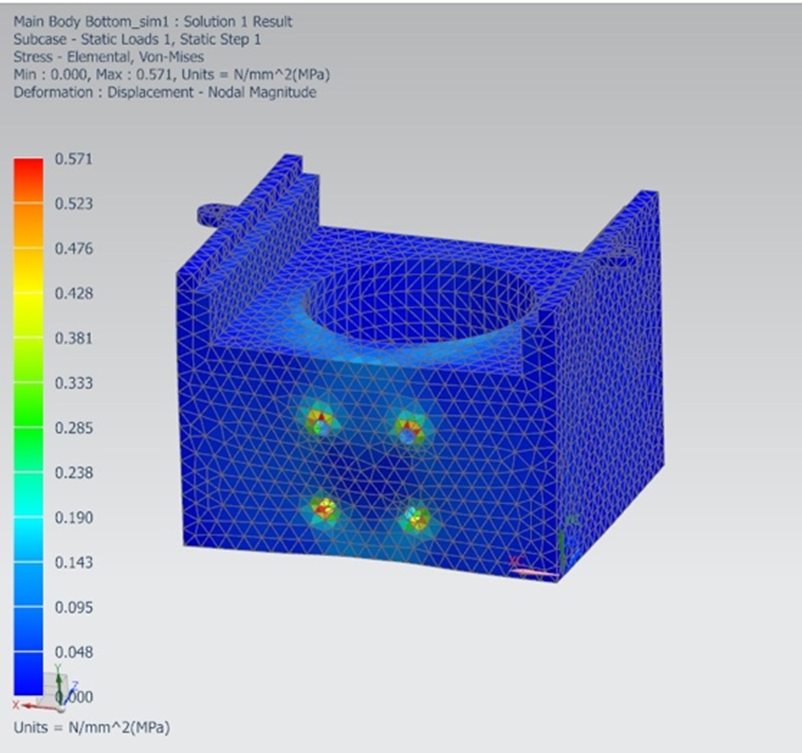
\includegraphics[width=0.5\linewidth]{mainbodybelowfinal.png}
    \caption{Analysis result of main body below part}
    \label{mainbodybelow}
\end{figure}

Thirdly, the bottom part of the main body is analyzed to determine the stress distribution. According to the analysis, except the sections which enable connection with the other parts, there is no stress concentration or propagation.
This part is one of the structurally critical parts that will hold the main structure, so it has a bulk structure. physically, this part is fixed to the table with the help of a clamp. Considering this situation during the analysis, fixed constraint was applied to the screw slots where the caliper will be mounted.  The load on the part is transferred from the pipe interface to which it is connected on the inside, so the force is applied to the connection interface as much as the load coming from the bottom. In order to increase the reliability of the analysis, the load capacity was multiplied by 1.5 to ensure the rigidity of the part against possible calculation errors.

\begin{figure}[h!]
    \centering
    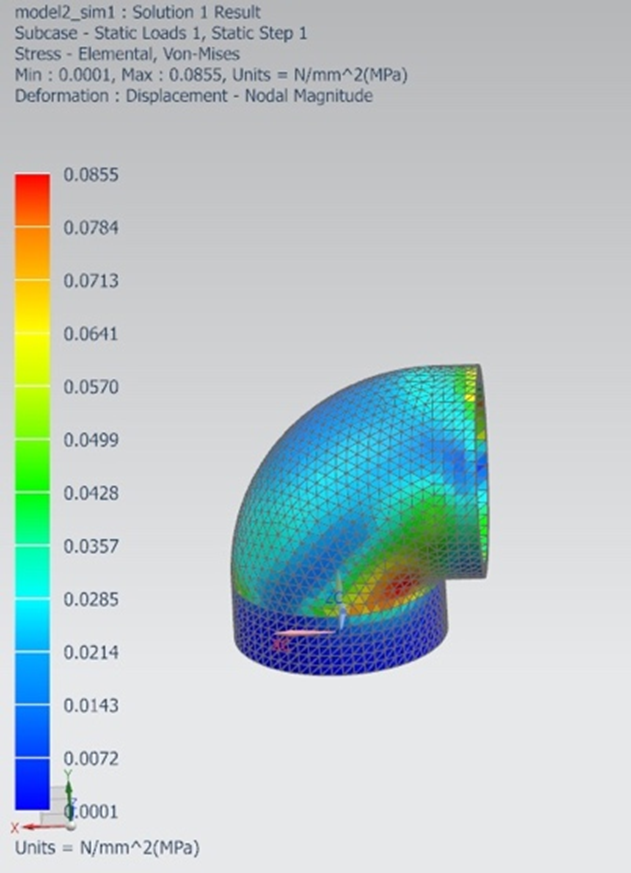
\includegraphics[width=0.5\linewidth]{elbowfinal.png}
    \caption{Analysis result of upper elbow}
    \label{fig:upperelbowfinal}
\end{figure}


The elbow of the pipe is analyzed to see if there are any excessive stresses. Most of its surface (except the red part) has low stress applied on it, according to the analysis. The red part has a stress of 0.0855 MPa.
\newpage

\begin{figure}[H]
    \centering
    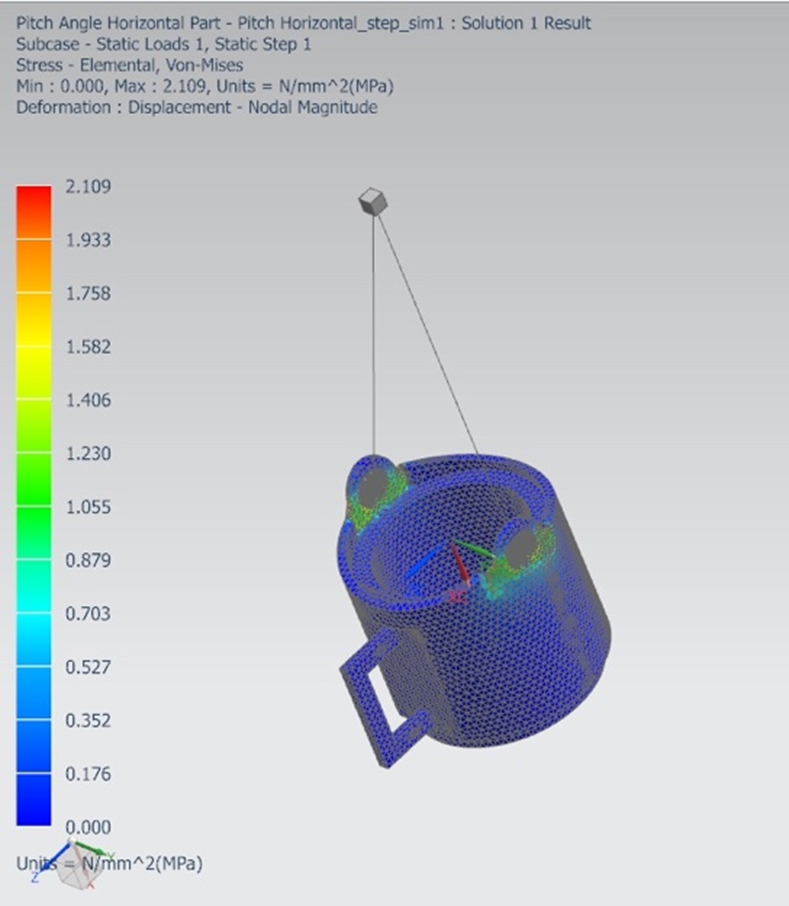
\includegraphics[width=0.6\linewidth]{pitchanglefixedfinal.png}
    \caption{Analysis result of the pitch angle fixed part}
    \label{fig:pitchanglefixedfinal}
\end{figure}

Finally, the horizontal part of the pitch angle is analyzed. According to the analysis, the part is under a stress less than 0.3-0.4 MPa, approximately. 
This part will provide the necessary connection to give the pitch angle. The part will be made of ABS plastic and during the analysis we used the interest of this part. All the weight of the moving head will flow through this connection point, so this is a structurally critical part. In order to simulate real life as accurately as possible, an analysis scenario is designed as follows. According to this scenario, the part has an interference fit connection with the elbow analyzed above. During the analysis, this interference fit surface was determined as a fixed constraint. The side that will connect with the moving part is attached to the connection surface with RB2 fasteners. The other end of the RB2s is connected to the point mass simulating the moving head. This point mass is in the same position as the center of gravity of the moving part. Finally, this structure was subjected to a load of 2 g vertically and 0.75 g laterally. When the analysis results were evaluated, no problems were observed.

\section{Discussion of Control Angorithms and Software}

The implemented Arduino program for the table tennis ball pitcher machine is designed to control motor speeds, ball spin, and orientation angles (pitch and yaw) using servo motors and stepper motors. The algorithm allows for user inputs to configure desired speeds, spins, and angles, ensuring dynamic and customizable ball launching operations.

\subsection{Explanations of Control Algorithms and Software}


\begin{figure}[H]
    \centering
    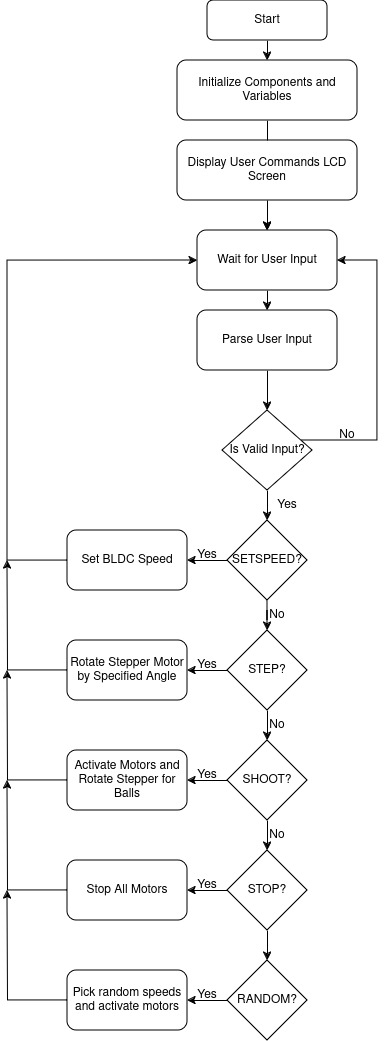
\includegraphics[width=0.5\textwidth]{CH5 figureler/salih figureler/main flow chart.jpg}
    \caption{Main flow chart}
    \label{fig:main flow chart}
\end{figure}

\subsubsection{Motor Speed Control Algorithm}
\begin{itemize}
    \item \textbf{Input:}  User-defined speed, spin effect, and spin direction
    \item  \textbf{Process:}
    \begin{itemize}
        \item Calculate target RPM for each motor based on spin direction.
        \item Map RPM values to ESC throttle range.
        \item Gradually adjust speeds for smooth transitions.
    \end{itemize}
    \item \textbf{Output:} Motors set to desired speeds for launching.
\end{itemize}

\begin{figure}[H]
    \centering
    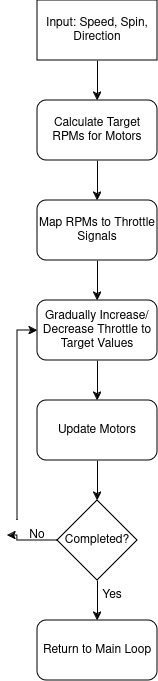
\includegraphics[width=0.25\textwidth]{CH5 figureler/salih figureler/BLDC Motor Control flow chart.jpg}
    \caption{BLDC Motor Control flow chart}
    \label{fig:BLDC motor control flow chart}
\end{figure}

\subsubsection{Stepper Motor Control for Yaw and Pitch Adjustments}
\begin{itemize}
    \item \textbf{Input:} Angle values for yaw and pitch received from commands.
    \item  \textbf{Process:}
    \begin{itemize}
        \item Calculate steps needed for the desired rotation.
        \item o	Move stepper motor incrementally for precision.
    \end{itemize}
    \item \textbf{Output:} Adjusted angles for the head orientation.
\end{itemize}

\begin{figure}[H]
    \centering
    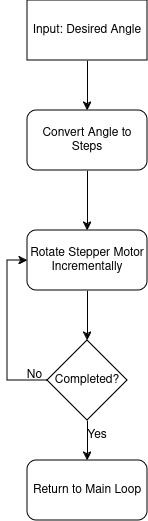
\includegraphics[width=0.2\textwidth]{CH5 figureler/salih figureler/Stepper motor control flow chart.jpg}
    \caption{Stepper motor control flow chart}
    \label{fig:Stepper motor control flow chart}
\end{figure}

\subsubsection{User Command Parser}

\begin{itemize}
    \item Parses commands from the serial interface or from the bluethooth IC for specific actions.
    \item Ensures data integrity before processing.
\end{itemize}

\textbf{Example Commands:}

\begin{itemize}
    \item \textbf{SETSPEED 5:} Sets stepper speed to 50 RPM.
    \item \textbf{STEP 45:} Rotates stepper motor by 45 degrees.
    \item \textbf{SPEED 1500 200 90 :} Sets base speed, spin effect, and spin direction.
\end{itemize}

\subsubsection{Motor Speed Calculation}
\begin{itemize}
    \item Computes RPMs for the three motors based on angular directions using trigonometric calculations:
\end{itemize}
\[RPM_i = \frac{\mathrm{BaseSpeed + SpinEffect} \cdot \cos(\theta_i - SpinDirection)}{r_{wheel} \cdot \frac{2\pi}{60}}\]

\subsubsection{Yaw and Pitch Control}
\begin{itemize}
    \item Uses servo motors to achieve precise angular control.
    \item Maps angle inputs to servo signal  based on resolution.
\end{itemize}

\begin{figure}[H]
    \centering
    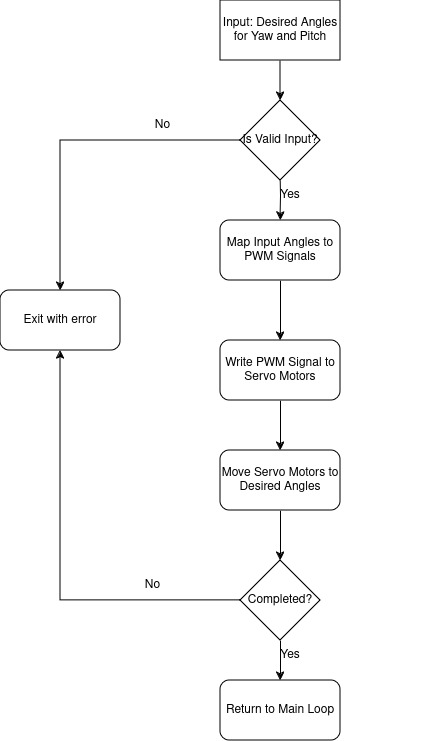
\includegraphics[width=0.40\textwidth]{CH5 figureler/salih figureler/yaw and pitch control flow chart.jpg}
    \caption{Yaw and pitch angle control flow chart}
    \label{fig:Yaw and pitch angle control flow chart}
\end{figure}

The control \textbf{ algorithms and software implementation} effectively allow for customizable ball pitching by integrating servo and stepper motor controls. Each subsystem is modular, ensuring scalability for future enhancements like additional spin modes, wireless interfaces, or advanced trajectory mapping.

\subsection{Explanation of the Circuit Design}
\subsubsection{Microcontroller (Arduino Rev3)}
\begin{itemize}
    \item The \textbf{Arduino Uno (Rev3)} serves as the \textbf{central controller} for the entire system.
    \item It receives \textbf{commands} from the user through serial communication and processes inputs for motor control, servo positioning, and trajectory adjustments.
    \item Multiple \textbf{PWM (Pulse Width Modulation) pins} are used to regulate motor speeds and servo positions.
    \item The \textbf{analog pins (A0-A10)} monitor inputs like potentiometers and sensors for adjustments.
\end{itemize}

\subsubsection{Motor Control System}
\paragraph{DC Motors for Ball Launching}
\begin{itemize}
    \item Three \textbf{Brushless DC motors (MT2204)} are controlled via HW-30A \textbf{ESC (Electronic Speed Controllers)}.
    \item ESCs (marked as A7, A8, A9) receive \textbf{PWM signals} from Arduino and translate them into motor speeds based on mapped input values.
    \item The motors are responsible for imparting \textbf{spin} and \textbf{speed} to the ball.
\end{itemize}

\paragraph{Stepper Motors for Pitch and Yaw Control}

\begin{itemize}
    \item A \textbf{Stepper Motor Driver (L298N)} is used to drive stepper motors for \textbf{yaw and pitch} adjustments.
    \item The \textbf{IN1-IN4} pins control the motor phases, while \textbf{ENB/ENA} enable the motor operation.
    \item Yaw and pitch angles are set through \textbf{commands} sent to the Arduino, which calculates the stepper steps based on the desired angles.
\end{itemize}

\subsubsection{Servo Motors for Fine Adjustments}

\begin{itemize}
    \item Servo motors (labeled as \textbf{J1 and J2}) handle \textbf{small angular adjustments} for finer control of pitch and yaw.
    \item These servos receive \textbf{PWM signals} directly from the Arduino and respond to changes in user inputs.
    \item They are used to refine angular positioning for precision targeting.
\end{itemize}

\subsubsection{Power Supply and Voltage Regulation}

\begin{itemize}
    \item The system is powered by an \textbf{external 12V DC source} connected through a \textbf{power plug}.
    \item A \textbf{voltage regulator} steps down the 12V input to \textbf{5V} required for Arduino and other components.
    \item The regulation circuit ensures \textbf{stable power delivery} to sensitive components.
\end{itemize}

\subsubsection{Input Controls and Sensors}

\begin{itemize}
    \item A \textbf{potentiometer (R1 - 10k{$\Omega$})} allows \textbf{manual control}  of angles and speeds, providing variable voltage outputs read by the Arduino’s \textbf{analog pins}.
    \item Resistors \textbf{R2 and R3 (1l{$\Omega$})} are used for \textbf{current-limiting} to protect sensitive components.
    \item Buttons and switches are connected for \textbf{manual triggers}, enabling users to initiate actions like ball shooting or stopping the motors.
\end{itemize}


\subsubsection{Communication and Signal Flow}

\begin{itemize}
    \item Signals from the \textbf{Arduino’s PWM and analog pins} are routed to motors, servos, and drivers, enabling control over:
    \begin{itemize}
        \item \textbf{Spin} by varying motor speeds.
        \item \textbf{Yaw and pitch angles} via stepper and servo motors.
        \item \textbf{Ball launch frequency} through motor activation timing.
    \end{itemize}
    \item Feedback loops allow the system to \textbf{adjust speeds and positions} dynamically based on user inputs.
\end{itemize}

\subsubsection{Functional Overview}

\begin{itemize}
    \item The circuit ensures \textbf{modular functionality} by dividing tasks into subsystems for \textbf{launch speed, spin, yaw/pitch control}, and user \textbf{inputs}.
    \item It provides \textbf{high precision} in controlling the trajectory of the ball and can adapt to different user configurations.
    \item The use of \textbf{PWM signals} and \textbf{stepper drivers} makes it scalable for future enhancements like \textbf{wireless control or advanced spin profiles}.
\end{itemize}

For the electricity part, in order to protect the device and its components, a glass fuse is inserted. If the supply excesses a certain amount, this glass fuse gets heated and burns out. Therefore, it loses its capability to conduct electricity and protects the device itself. informs that the supplied current should be reduced. 

The device works at 10 V. However, it is desired to work the device by mains voltage, which is approximately 230 V. To be able to work the device by the mains voltage, a voltage stepper adapter is to be used to lower the voltage value to the desired value, which is 10 V.




\section{Optimization}
In the optimization part, some procedures of optimization carried out for the design will be reported. The parameters to be satisfied, the iterative processes, how the results differ with each iterative step and the final optimal results will be mentioned.

The design utilizes a 3-wheel system to launch the balls. As the surface of table tennis balls are very smooth, the wheels’ surface should be covered with a material that has a good grip so as to transfer the velocity of the wheels to balls with maximum efficiency. This resulted in a trial-and-error process for material selection. The material tried first was sponge. However, the tests conducted showed that, at high speeds, wear was observed on the material surface. To overcome this situation, rubber was tried next. After conducting some tests using this material, it was found that high amount of wear was prevented on the surface, providing a more stabilized launch. 

Another process of optimization involved the Maltese wheel system used to feed the balls from storage to feed. This process needed to be smooth and fast, as it played a part in setting the frequency for the ball launch. In the first step, a Maltese wheel with 8 segments was tried, however, it was observed that the system was jammed from time to time and failed to launch the balls. A solution proposed was to try to decrease the segment size, so a 6-segmented Maltese wheel was tried nest to see if this problem can be prevented. As a result, the 6-segmented Maltese wheel enabled the balls to be transmitted smoothly, without any jamming. 

Also, the wheels are aligned in a more convenient way. For the wheel dimensions decided, the speed of the ball did not turn out to be at the desired range, it was too high. To lower the speed, the wheels were made smaller. For the same angular velocity, a smaller linear velocity is obtained in that way, so the requirements are satisfied.

The pipe was manufactured in a gapped fashion in order to observe whether there exists a notch, or any type of texture anomalies. Capability of determining this type of anomaly provides an early response to the issue, which saves time and cost as well. 

Another gapped structure approach was used at the section where the wheels are located. This feature enables flexibility in terms of aligning the wheels and trajectional variety while launching.  

It should be noted that the system was made of intermeshing pieces, rather than a complete structure. The main purpose is to provide flexibility, in other words, if one part has an issue in terms of tolerances or dimensions, the necessity to manufacture the whole part is prevented. In this case, remanufacturing only the relevant part is sufficient to overcome the problem. Therefore, this optimization is beneficial in terms of time and cost.

\section{System to Be Manufactured}
The production phase starts from the launcher section. This is because the launcher part contains more complex components, and since the design is generally structured in an interlocking manner, it is important to start from one end and proceed to the other. Additionally, considering that the prototype’s speed and spin functions will be evaluated first through the launcher section, it is logical to start from here. The launcher consists of a 4-piece structure with three motor connection components integrated into the main part.
After the launcher, there exists a section with the pitch angle gear and motor mounted on it , connected via a pin. This section provides housing for these components and also helps attach the launcher to the elbow joint in a vertically movable way. This part is also produced using additive manufacturing. The gear pair that assists in adjusting the pitch angle includes one gear connected to the motor shaft and the other to the pin connection point. The gears are manufactured using additive manufacturing techniques.
At the rear, a joint structure connects the yaw angle mechanism to the pitch angle section.
The yaw angle is provided through the neck section, again with the help of a gear pair. One of these gears is mounted on the neck, while the other is externally connected to the motor. Two bearings, housed within a box-like structure, prevent the gears and the neck from slipping. The bearings are also tightly press-fitted into the neck.
Underneath this, there is a maltese wheel mechanism for feeding the balls. The edges of the tube where the maltese wheel is located are designed with openings to allow for intervention in case of jamming. Additionally, at the curved section of this tube, there is a part where the feeding motor is housed. The wheel is manufactured using additive manufacturing, featuring six arms.
For the connection between the wheel and the storage section, a grooved structure was designed to allow the balls to slide into the feeding area. This structure enables the feeding
section to be connected smoothly without sticking. There are connection points on both sides of the mentioned box section and the groove structure. These connection points are designed as G Clamps with a single pin structure based on necessary analyses.
The storage section is connected to a mesh structure. This mesh is designed in such a way that it is not at its most stretched state, allowing the balls to return more easily.


\section{Sustainability Analysis}
The sustainability analysis is conducted by assessing material options to prioritize recyclability and environmental impact. Energy efficiency is addressed through the selection of optimized motors and control mechanisms. The design is refined to minimize material usage, enhance ease of disassembly, and ensure recyclability. A ball recycling system is integrated to reduce waste and improve operational efficiency, aligning the project with sustainability objectives. The whole system is analyzed in terms of sustainability through SolidWorks, and results of the analysis are summarized below. The entire analysis report is presented in the Appendix.

\begin{figure}[h]
    \centering
    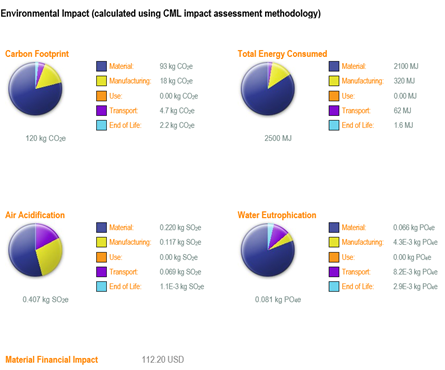
\includegraphics[width=0.6\textwidth]{sustaibabilityanalysis.png}
    \caption{Results of the Environmental Impact Analysis}
    \label{fig:sustainabilityanalysis}
\end{figure}

\newpage

\section{Test Plan}
Tests are planned to evaluate the design criteria. Proper tests are designed with relevant information, and specifications. These are created to demonstrate the project design meets the predetermined design criteria. Details of the test setup, measurement devices, and expected results are presented below corresponding to each design criteria.

\subsection{Serving Speed (13\%)}
The ball must reach a maximum speed of 30 m/s during launch. It must be adjustable within this range. The test involves recording the ball's launch using a slow-motion camera. The board, placed in the ball’s trajectory path, helps track the ball’s distance over time. By analyzing the video footage, the distance the ball travels within a set time frame (e.g., 1 second) is measured using the 5 cm intervals on the board. The translational speed is then calculated by dividing the distance traveled by the time taken. The equipment required for this test includes a slow-motion camera to capture the ball’s launch and a board with vertical lines marked at 5 cm intervals to measure the ball’s movement. The calculated ball speed should match the specified maximum speed of 30 m/s. Additionally, the speed should be adjustable within this range. The result will confirm whether the system is capable of achieving the required ball speed and adjustability for professional training.
\subsection{Throwing Frequency (13\%)}
The ball’s launch frequency must provide 60 balls per minute. It must be adjustable within this range. To test the adjustability of the ball-throwing frequency, the machine is configured to its minimum, midpoint, and maximum frequency settings. A stopwatch is used to count the number of balls launched over a 60-second period for each setting. The test is repeated three times for each frequency to ensure consistency and accuracy in the results. The equipment required for this test includes a stopwatch to measure the time and count the number of balls launched, along with the ball-throwing machine configured at different frequency settings. The results should confirm that the system can launch 60 balls per minute at the maximum frequency setting and that the frequency is adjustable within this range. The test should verify that the system allows smooth and accurate adjustments, meeting the specified frequency requirements for training professional players.

\subsection{Spin Type and Amount (10\%)}
The ball must be able to be given spin up to 500 RPM, including backspin, topspin, sidespin, and their derivatives. This spin value must be independent of speed. The system’s ability to provide adjustable spins is tested by setting the machine to generate different spin types (topspin, backspin, sidespin, and their combinations) at various speeds. The rotational speed of the ball is measured using a tachometer or high-speed camera to ensure the spin reaches up to 500 RPM and remains independent of the ball’s velocity. The test is repeated for all combinations of spins to assess the system's performance. The equipment needed for this test includes a tachometer or high-speed camera to measure the ball’s rotational speed and the ball-throwing machine configured to generate different spin types at various speeds. The results should confirm that the system is capable of generating the required spins (topspin, backspin, sidespin, and combinations) with rotational speeds of up to 500 RPM. The spin should remain independent of the ball’s translational speed, verifying that the system meets the spin control requirements accurately and consistently across different spin configurations.

\subsection{Yaw Angle Adjustment (7\%)}
The launcher must provide launch with a yaw angle within a range of ±20 degrees horizontally. The test involves adjusting the launcher to various yaw angles within the ±20-degree range. After each adjustment, the ball’s landing positions on the opposite side of the table are recorded. This process is repeated multiple times for different angles to verify that the system provides sufficient horizontal coverage across the entire table. The test is designed to check the consistency and accuracy of the yaw angle adjustment. The equipment required for this test includes a measuring device to record the ball’s landing positions on the opposite side of the table, and a setup that allows the launcher to adjust its yaw angle within the specified range of ±20 degrees. The results should confirm that the ball lands within the desired areas on the opposite side of the table, verifying that the system provides a yaw angle range of ±20 degrees. The test will also ensure that the system can consistently adjust the yaw angle and achieve accurate performance, meeting the specified requirement for horizontal.

\subsection{Pitch Angle Adjustment (7\%)}
The launcher must provide launch with a pitch angle within a range of 0 to -20 degrees vertically. To test the adjustable pitch angle, the launcher is set to various pitch angles within the range of 0 to -20 degrees. After each adjustment, the landing positions of the balls on the opposite side of the table are recorded. The test is performed at multiple pitch angles to ensure that the system provides consistent and accurate vertical coverage. The results are then analyzed to confirm that the balls land in most areas on the opposite side of the table. The equipment required for this test includes a measuring device to record the ball's landing positions on the opposite side of the table and a launcher with adjustable pitch angle settings. The results should demonstrate that the system can launch balls with pitch angles within the specified range of 0 to -20 degrees, ensuring vertical coverage across the table. The test will verify that the system consistently provides accurate launch angles, meeting the requirement for adjustable pitch angles and proper vertical distribution of the ball's landing position.

\subsection{Storage Capacity (6\%)}
There should be 60 balls in storage. The box is filled with the required number of balls, and it is inspected to see if the box volume is enough. The box, the balls and a measurement device to have information about the dimensions of the storage. . The box has the capacity to carry 70 balls, which is determined by putting 60 balls initially, then the empty volume is filled with more balls.

\subsection{Weight (4\%)}
The maximum weight of the entire system must not exceed 25 kilograms. The test involves weighing each individual component of the system using the calibrated digital scale before assembly. The weight of each component is compared to the limits specified by the ISO-FDIS-11228 ergonomics standards. Once the system is fully assembled, the total weight is measured to ensure it does not exceed the 25-kilogram limit. This process is repeated to verify consistency and confirm that all weight limits are appropriate. The equipment required for this test includes a calibrated digital scale to measure the weight of each system component individually before assembly, as well as the scale to weigh the entire assembled system. The results should confirm that each component's weight is within the prescribed limits according to ISO-FDIS-11228 standards, and that the total weight of the assembled system does not exceed 25 kilograms. This test ensures that the system complies with ergonomic weight requirements for ease of handling and transport.

\subsection{Stability of the System (6\%)}
The system is securely fastened to the table or floor in the middle of the opponent’s side of the ITTF standard table, at the center of the width of the table. The maximum displacement after 50 throws shall be 20 mm. The mounting position is tested by securely fastening the system to the ITTF standard table at the center of the opponent's side, ensuring that it is rigidly mounted. After mounting, the system is operated, launching 50 balls in succession. The displacement of the system from its original position is measured using a precision displacement sensor or other measuring tools. The displacement should not exceed 20 mm after 50 throws. This test is repeated to ensure consistent results and verify that the system maintains stability and adheres to the displacement limit. The equipment required for this test includes a precision displacement sensor or measuring tools (such as a ruler or caliper), a mounting system, and the ITTF standard table. The results should confirm that the system remains securely mounted, with the displacement not exceeding the 20 mm limit after 50 throws. This ensures that the mounting system is stable and rigid, as specified in the requirement.
\subsection{Ball Durability (4\%)}
The lifetime of a single ball in the cycle should be at least 1000 throws. The test involves launching the balls at various speeds and angles using the system to simulate normal operation. After 1000 throws, each ball is inspected for signs of wear, such as cracks or deformation. The table's surface is also examined for any damage, including scratches or dents. The test is repeated multiple times using different balls to ensure consistency and to verify that the system does not cause any damage to the table or balls during operation. The equipment needed for this test includes a set of tennis balls, the ball-launching system, and inspection tools such as a magnifying glass or microscope to check for damage on the balls and a visual inspection for any damage to the table surface. The results should confirm that the balls exhibit no signs of wear or damage after at least 1000 throws and that the table surface remains undamaged, with no visible scratches or dents. This test ensures that the system meets the requirement of not damaging either the table or the tennis balls during its operation.
\subsection{Control Accuracy and Output Consistency (7\%)}
The system must have a user interface allowing launch parameter configuration with a maximum 10\% deviation. The test involves inputting various ball throw parameters, such as impact location, speed, and spin, into the system’s user interface. The ball's actual launch speed, spin, and impact location are then measured using the appropriate sensors. The entered values are compared to the actual results to determine if the deviation between the input and output parameters exceeds the maximum allowed limit of 10\%. This process is repeated for multiple sets of parameters to ensure the system consistently meets the deviation requirement. The equipment required for this test includes the user interface of the system, sensors to measure the ball's launch speed, spin, and impact location, and a system for comparing the entered input parameters to the actual launch parameters. The results should confirm that the system's actual launch parameters do not deviate by more than 10\% from the input parameters. The test will verify that the user interface is accurate and responsive, meeting the requirement for configurable launch parameters within the specified deviation limit.
\subsection{Ball Recyclability (5\%)}
The design can collect the properly returned balls from the player. Recyclable ball height needs to be at least 1 meter. The collector mechanism is tested by simulating a scenario where balls are returned by the player from the opposite side of the table. The system should effectively collect all returned balls. The height of the recyclable ball collection area is measured to ensure it reaches at least 1 meter. Balls are returned at various speeds and angles, and the performance of the collector is observed to verify that all balls are properly captured. The test is repeated under different conditions to ensure consistency and verify the 1-meter height requirement. The equipment required for this test includes a 1-meter-long net to cover the side opposite the player, and the collector mechanism for capturing the balls. The results should confirm that the system can collect all returned balls efficiently and that the recyclable ball collection area reaches a height of at least 1 meter. This ensures that the design meets the specified requirements for ball collection and height.

\subsection{Compliancy with Standards (3\%)}
The system is compliant with ITTF table and ball dimensions: Suitable for a 2.74 m long and 1.525 m wide table, can serve over a 15.25 cm high net and suitable for standard table tennis balls with a 2.7-gram weight and 40 mm diameter. To test compliance with ITTF standards, the system is placed on a table that is 2.74 meters long and 1.525 meters wide to verify proper fit. The system is then tested with a 15.25 cm high net to ensure that the balls clear the net during launch. Standard table tennis balls with a weight of 2.7 grams and a diameter of 40 mm are used to confirm that the system handles and launches them accurately. The equipment required for this test includes a table with dimensions of 2.74 meters in length and 1.525 meters in width, a 15.25 cm high table tennis net, and standard 2.7-gram, 40 mm diameter table tennis balls. The results should confirm that the system fits properly on the specified table dimensions, launches balls that clear the 15.25 cm high net, and functions correctly with standard table tennis balls. This ensures that the system meets the ITTF specifications for table and ball dimensions and adheres to the standard table tennis rules.

\subsection{Power Consumption (3\%)}
The machine should operate on standard mains electricity (220-240V, 50-60 Hz). Also, it should not consume more than 2000W.  The system is connected to a standard mains electricity supply (220-240V, 50-60 Hz), and a power meter is used to measure its electrical usage during operation. The system is run under typical operating conditions, and the total power consumption is recorded. The measurement is analyzed to ensure that the system’s power consumption does not exceed 2000W. The equipment required for this test includes a power meter to measure the system's total power consumption, and a standard mains electricity supply (220-240V, 50-60 Hz). The results should confirm that the system’s power consumption remains within the specified limit of 2000W while operating under typical conditions. This test ensures that the system complies with the requirement for minimized power consumption.

\subsection{Budget (8\%)}
Total spending for the prototype of the design should be kept within 300 USD. The total cost of the system is tested by tracking all expenses related to the design and prototype construction. Each component and material used in the system is priced, and the total spending for the prototype is calculated. The final cost is then compared to the assigned budget to ensure it does not exceed the 300 USD limit. This process is repeated to verify that all costs are accurately accounted for. The equipment required for this test includes a list of all components and materials used in the design, as well as access to pricing information for each item. A calculator or spreadsheet software is necessary to track and calculate the total expenses. The results should confirm that the total spending for the prototype does not exceed the 300 USD budget. This test ensures that the system is developed within the financial constraints, meeting the cost requirement.

\subsection{Portability (4\%)}
The design, when unassembled, should fit inside a 1 m3 box. The test involves disassembling the system and measuring its components to ensure they fit comfortably inside a 1 m³ box. The dimensions of the unassembled system are compared to the box's size to confirm it fits within the specified volume. Additionally, one person should attempt to transport the box to ensure that it is lightweight and manageable for a single individual. The equipment required for this test includes a measuring tape or ruler to measure the dimensions of the unassembled system, a 1 m³ box, and a person to test the portability by carrying the box. The results should confirm that the system, when unassembled, fits inside the 1 m³ box and can be transported by one person. This test ensures that the design is portable and meets the requirement for easy transportation.

\section{Standards Used For Design Procedures and Performance Evaluation }
\subsection{Design Standards}
Standards utilized during the design stages of the table tennis ball pitching machine project are as follows:
\begin{itemize}
    \item \textbf{ISO 286-2:2010, Geometrical Product Specifications (GPS) – ISO code system for tolerances on linear sizes – Part 2: Tables of standard tolerance classes and limit deviations for holes and shafts}
    This standard was used for defining tolerances for shafts and housing diametric fits, ensuring compatibility between the mechanical components. It specifically guided the selection of tight fits required for bearing seats in our design.
    
    \item \textbf{ISO 281:2007, Rolling Bearings – Dynamic Load Ratings and Fatigue Life}
    Applied in the selection of ball bearings to ensure they meet dynamic load requirements and have sufficient operational life under the defined conditions of the project.
    
    \item \textbf{ISO 12100, Safety of Machinery – General Principles for Design – Risk Assessment and Risk Reduction}
    Incorporated to ensure that the design adheres to essential safety principles, reducing risks to operators during use.
    
    \item \textbf{ISO 129, Technical Drawings – Indication of Dimensions and Tolerances}
    Used for ensuring clear and unambiguous communication of dimensions and tolerances on engineering drawings for manufacturing.
    
    \item \textbf{ISO 11228-1, Ergonomics – Manual Handling – Part 1: Lifting and Carrying}
    This was referenced to maintain ergonomic limits for weight and handling of portable components, ensuring compliance with manual handling standards.
    
    \item \textbf{ISO 527, Plastics – Determination of Tensile Properties}
    Used to assess and validate the mechanical properties of polymers selected for non-load-bearing components, such as housing or feed mechanisms.
    
    \item \textbf{AGMA 2000-A88, Gear Classification and Inspection – Gear Tooth Tolerances}
    Used for defining tolerances and quality standards for gear-based yaw and pitch control mechanisms in the design.
    
    \item \textbf{ITTF Equipment Standards, International Table Tennis Federation Standards for Balls and Tables}
    Ensured compliance with official table tennis equipment specifications for ball size, weight, and bounce characteristics.
    
    \item \textbf{ITTF Equipment Compatibility}
    The machine must work seamlessly with ITTF-approved tables. Also, the machine should ensure the compatibility of the machine with official table tennis balls.
    
    \item \textbf{Material: ABS plastic or celluloid}
    These materials are lightweight and durable, ensuring consistent bounce and spin performance.
    
    \item \textbf{Diameter: 40.0 mm ± 0.5 mm}
    Ensures compatibility with the ball launcher and maintains standard gameplay conditions.
    
    \item \textbf{Weight: 2.7 g ± 0.1 g}
    Launcher mechanisms are calibrated to handle this weight range for accurate operation.
    
    \item \textbf{Bounce Height: 24–26 cm}
    Used for testing ball performance and launcher accuracy during operation. If a ball is dropped from 30.5 cm, its rebound must comply. This is critical for evaluating ball trajectory accuracy.
\end{itemize}
\subsection{Performance and Test Standards}
The following standards and procedures were utilized or referenced for performance evaluation and testing of the project:
\begin{itemize}
    \item \textbf{ISO 14468-1:2015, Table Tennis – Playing Tables – Requirements and Test Methods}
    Applied to test the compatibility of ball trajectory and yaw-pitch mechanisms with official table tennis table specifications.
    
    \item \textbf{ASTM F2056, Standard Test Method for Table Tennis Ball Rebound Resilience}
    Used to measure the rebound consistency and performance of balls propelled by the machine.
    
    \item \textbf{ISO 60335-1, Household and Similar Electrical Appliances – Safety}
    Referenced for evaluating the electrical safety of the power supply and motorized systems.
    
    \item \textbf{ISO 9283, Robots and Robotic Devices – Performance Criteria and Related Test Methods}
    Used to measure repeatability and accuracy of the ball pitching mechanism across different settings.
    
    \item \textbf{ISO 14001, Environmental Management Systems – Requirements with Guidance for Use}
    For ensuring sustainable practices in material selection and manufacturing.
    
    \item \textbf{ISO 50001, Energy Management Systems}
    To evaluate and improve the energy efficiency of the machine.
\end{itemize}
By following these standards, the design and evaluation procedures of the table tennis ball pitching machine ensure safety, reliability, and adherence to international norms.
\section{Discussion and Conclusion}
In this report, the detailed design for the Automatic Table Tennis Ball Pitcher Machine project was documented. The design process required a lot of thought and meticulous work, as there were many components that had to work in unison, which called for taking many things such as geometries of the parts, kinematics and mechanics into careful consideration. Several parts required processes of optimization, which was mentioned in the report. Calculations and simulations to justify the predicted behavior of the system were performed, and analyses were run to clearly present the mechanical characteristics of the components. Test plans to evaluate the product were laid out, control algorithms were presented and sustainability analyses were detailed. How the parts would be manufactured, and the material selections were also discussed.
As the design process took many trial-and-error procedures and brainstorming, several ideas were filtered, scrapped or reimagined to obtain the best or close to best possible solutions to all the subfunctions and the overall system in general. Using the valuable experience gained from this, it would be wiser to approach the system as a whole from the start to be able to better foresee the problems that may arise for the assembly and manufacturing steps or better visualize the system for the analyses part for the components. As the system consists of many components, it helps to think and imagine the system in its entirety to be able to take the interactions of the components into consideration, or to better understand the contributions of different parts to calculations. Furthermore, having a better understanding of manufacturing processes and engineering practices might be helpful in decision processes, as having these insights from the start would be of use when coming up with new ideas, and keep in mind what is possible or what is more difficult to do in real life practice. The brainstorming sessions would be more fruitful, and the initial design step would progress much faster.
To conclude, it should be said that the whole design process was beneficial, as it presented an actual engineering challenge, where many factors had to be taken into account, and engineering knowledge accumulated up until now and other knowledge obtained through research had to be used together to bring solutions to different problems and requirements. If the project were to be done from the start, the experience gained throughout would make it so that it would proceed faster and in a more grounded way, which is a very valuable achievement for engineering notion.

\section{References}

\section*{References}

\begin{enumerate}

    \item Budynas, R. G., \& Nisbett, J. K. (2021). \textit{Shigley’s Mechanical Engineering Design.} McGraw Hill Education.

    \item Steyr, \textit{Steyr Technical Manual 282 E Bearing Catalog.} Steyr, 1981.

    \item Hibbeler, R. C. (2019). 
    \textit{Mechanics of Materials.} Pearson.
    
    \item ISO 286-2:2010, \textit{Geometrical Product Specifications (GPS) – ISO code system for tolerances on linear sizes – Part 2: Tables of standard tolerance classes and limit deviations for holes and shafts.} International Organization for Standardization (ISO). Available at: \url{https://www.iso.org/standard/37731.html}

    \item ISO 281:2007, \textit{Rolling Bearings – Dynamic Load Ratings and Fatigue Life.} International Organization for Standardization (ISO). Available at: \url{https://www.iso.org/standard/31149.html}

    \item ISO 12100:2010, \textit{Safety of Machinery – General Principles for Design – Risk Assessment and Risk Reduction.} International Organization for Standardization (ISO). Available at: \url{https://www.iso.org/standard/51528.html}

    \item ISO 129-1:2018, \textit{Technical Product Documentation – Indication of Dimensions and Tolerances – Part 1: General Principles.} International Organization for Standardization (ISO). Available at: \url{https://www.iso.org/standard/68189.html}

    \item ISO 11228-1:2003, \textit{Ergonomics – Manual Handling – Part 1: Lifting and Carrying.} International Organization for Standardization (ISO). Available at: \url{https://www.iso.org/standard/31143.html}

    \item ISO 527:2019, \textit{Plastics – Determination of Tensile Properties.} International Organization for Standardization (ISO). Available at: \url{https://www.iso.org/standard/75894.html}

    \item AGMA 2000-A88, \textit{Gear Classification and Inspection – Gear Tooth Tolerances.} American Gear Manufacturers Association (AGMA). Available at: \url{https://www.agma.org/}

    \item ITTF Equipment Standards, \textit{International Table Tennis Federation Standards for Balls and Tables.} International Table Tennis Federation (ITTF). Available at: \url{https://www.ittf.com/}

    \item ISO 14468-1:2015, \textit{Table Tennis – Playing Tables – Requirements and Test Methods.} International Organization for Standardization (ISO). Available at: \url{https://www.iso.org/standard/63277.html}

    \item ASTM F2056, \textit{Standard Test Method for Table Tennis Ball Rebound Resilience.} ASTM International. Available at: \url{https://www.astm.org/}

    \item ISO 60335-1:2020, \textit{Household and Similar Electrical Appliances – Safety – Part 1: General Requirements.} International Organization for Standardization (ISO). Available at: \url{https://www.iso.org/standard/72579.html}

    \item ISO 9283:1998, \textit{Robots and Robotic Devices – Performance Criteria and Related Test Methods.} International Organization for Standardization (ISO). Available at: \url{https://www.iso.org/standard/16737.html}

    \item ISO 14001:2015, \textit{Environmental Management Systems – Requirements with Guidance for Use.} International Organization for Standardization (ISO). Available at: \url{https://www.iso.org/standard/60857.html}

    \item ISO 50001:2018, \textit{Energy Management Systems – Requirements with Guidance for Use.} International Organization for Standardization (ISO). Available at: \url{https://www.iso.org/standard/69426.html}
\end{enumerate}





\newpage

\section{Appendices}

\begin{appendices}

\section{Technical Drawings}

\begin{figure}[H]
    \centering
    \includegraphics[width=0.9\textwidth]{özge_assembly1.png} % Replace with your file name
    \caption{Technical drawing of the assembly of the system}
    \label{fig:technical-drawing}
\end{figure}

\begin{figure}[H]
    \centering
    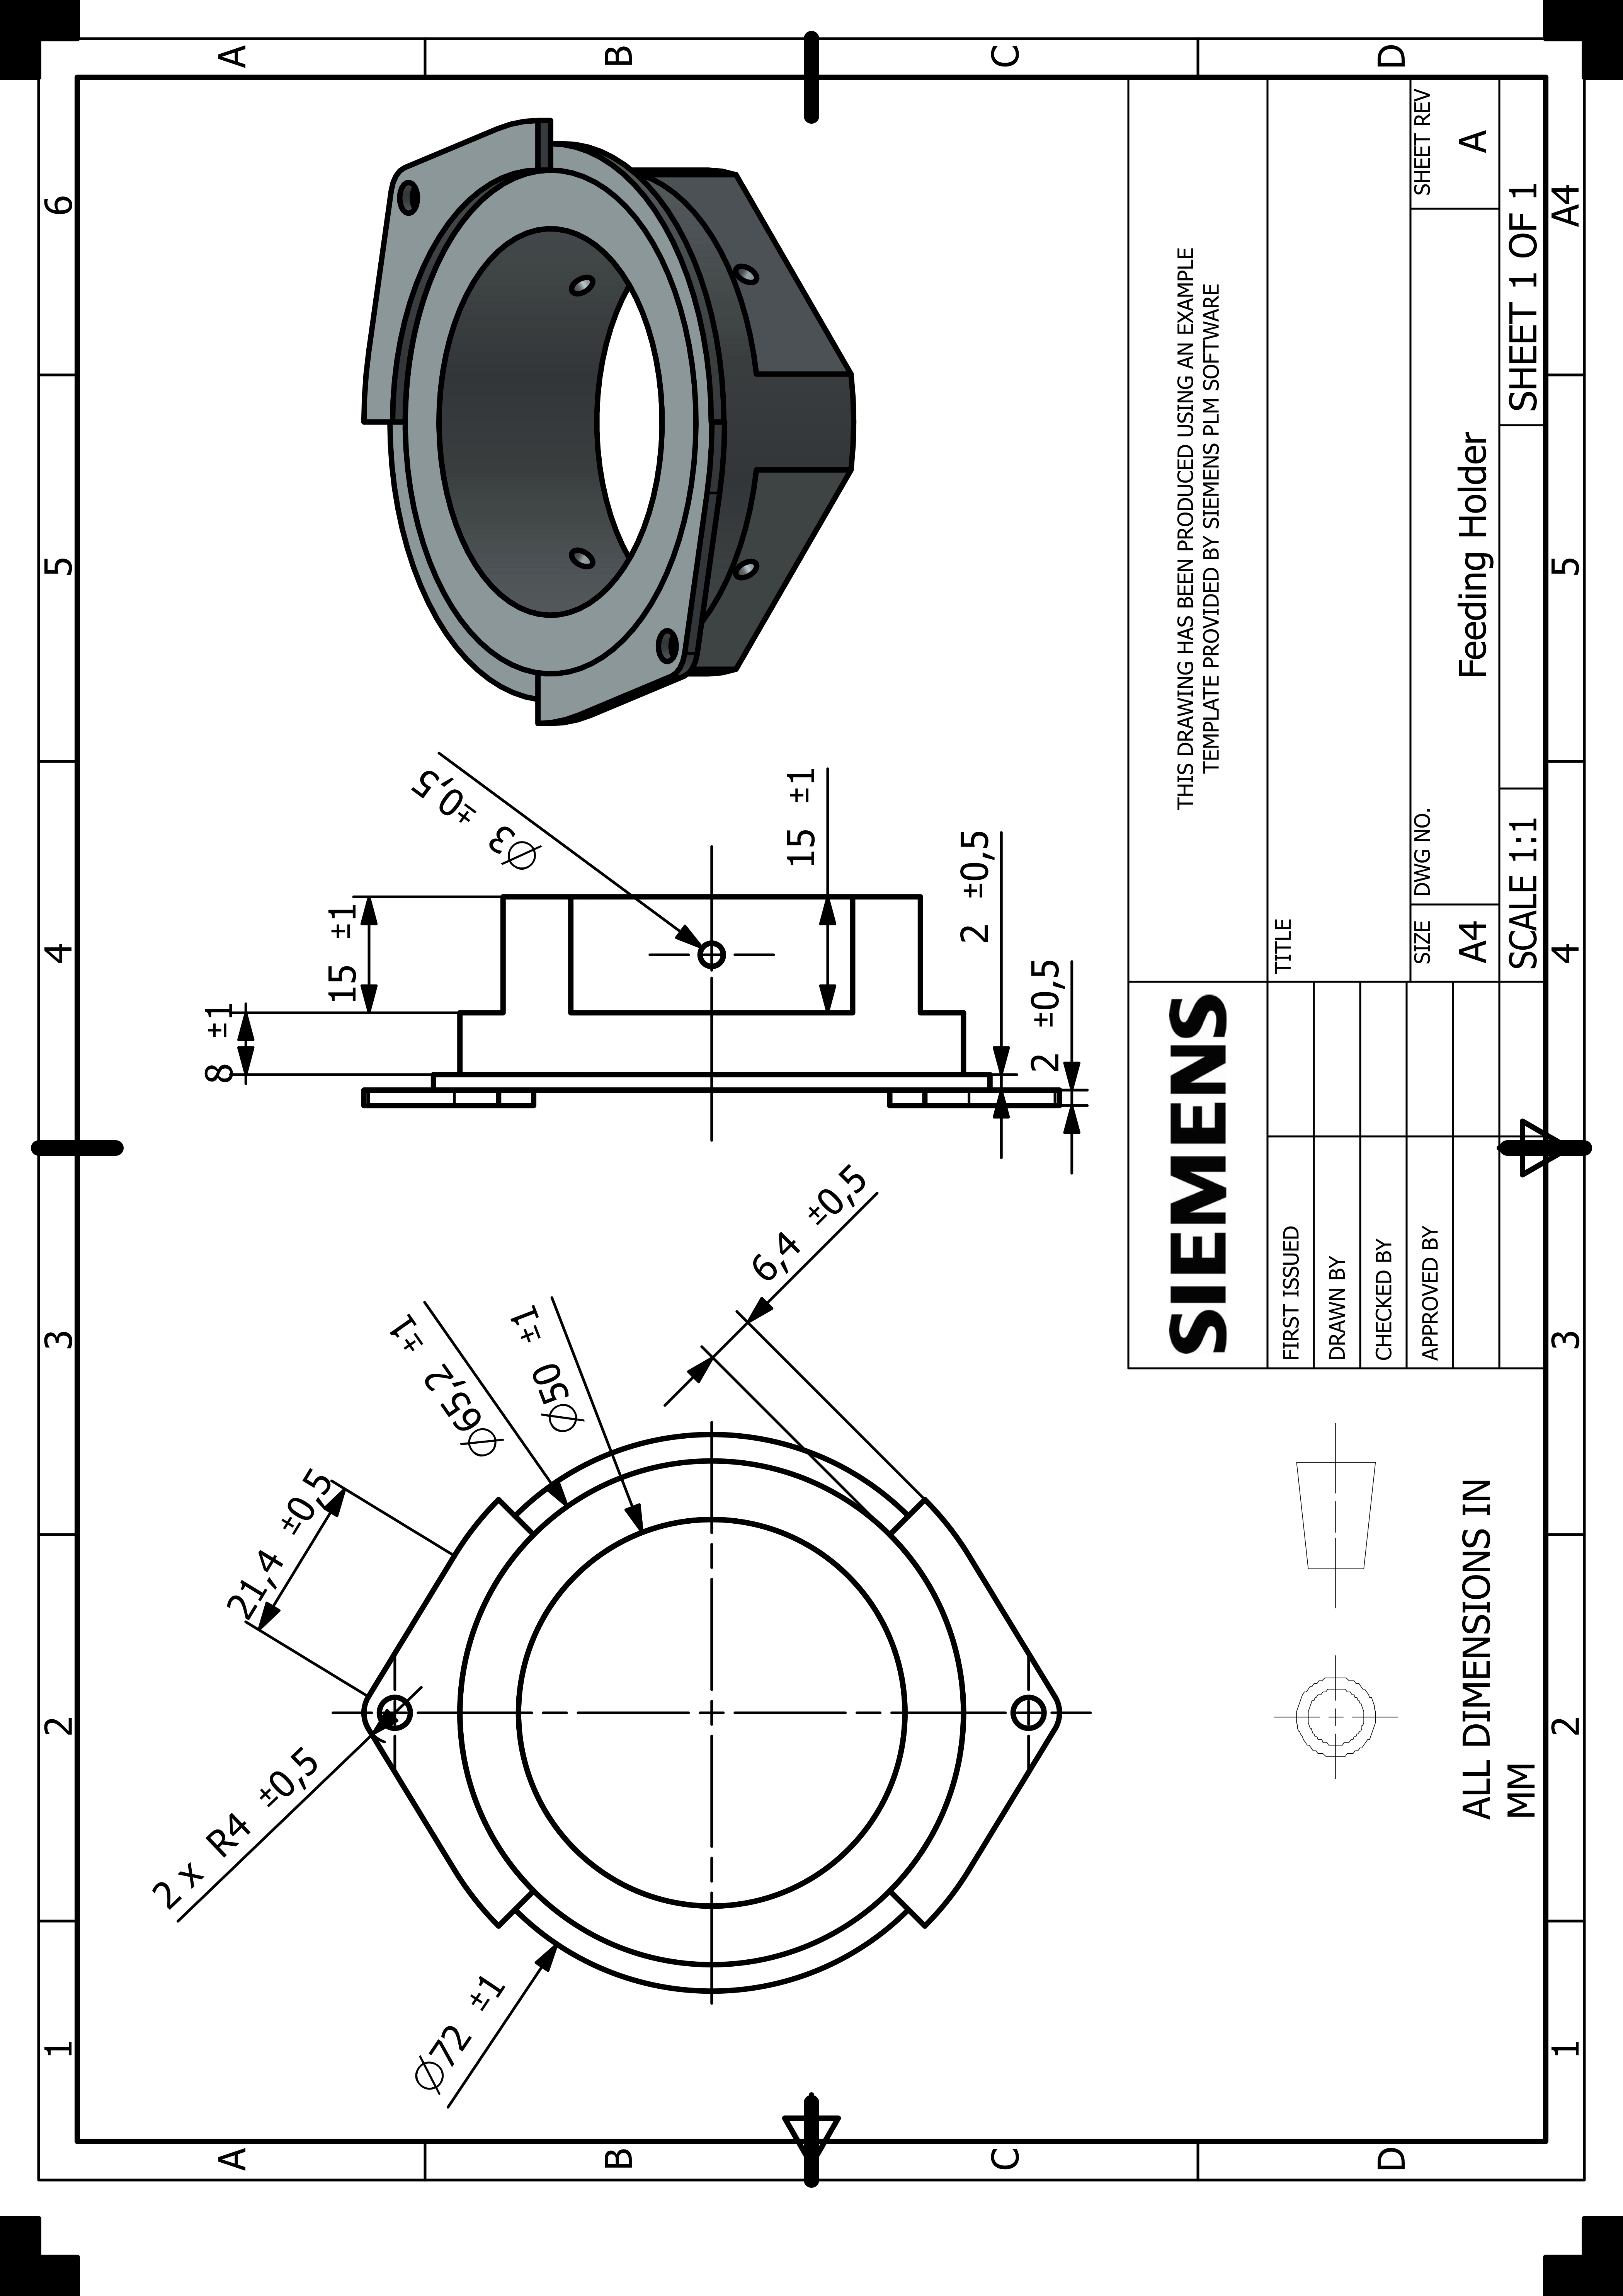
\includegraphics[width=\textwidth]{HP_Feeding Holder.png} 
    \caption{Technical drawing of the feeding holder}
    \label{fig:technical-drawing}
\end{figure}

\begin{figure}[H]
    \centering
    \includegraphics[width=\textwidth]{özge_yawmotoryatak.png} 
    \caption{Technical drawing of the yaw motor housing}
    \label{fig:technical-drawing}
\end{figure}

\begin{figure}[H]
    \centering
    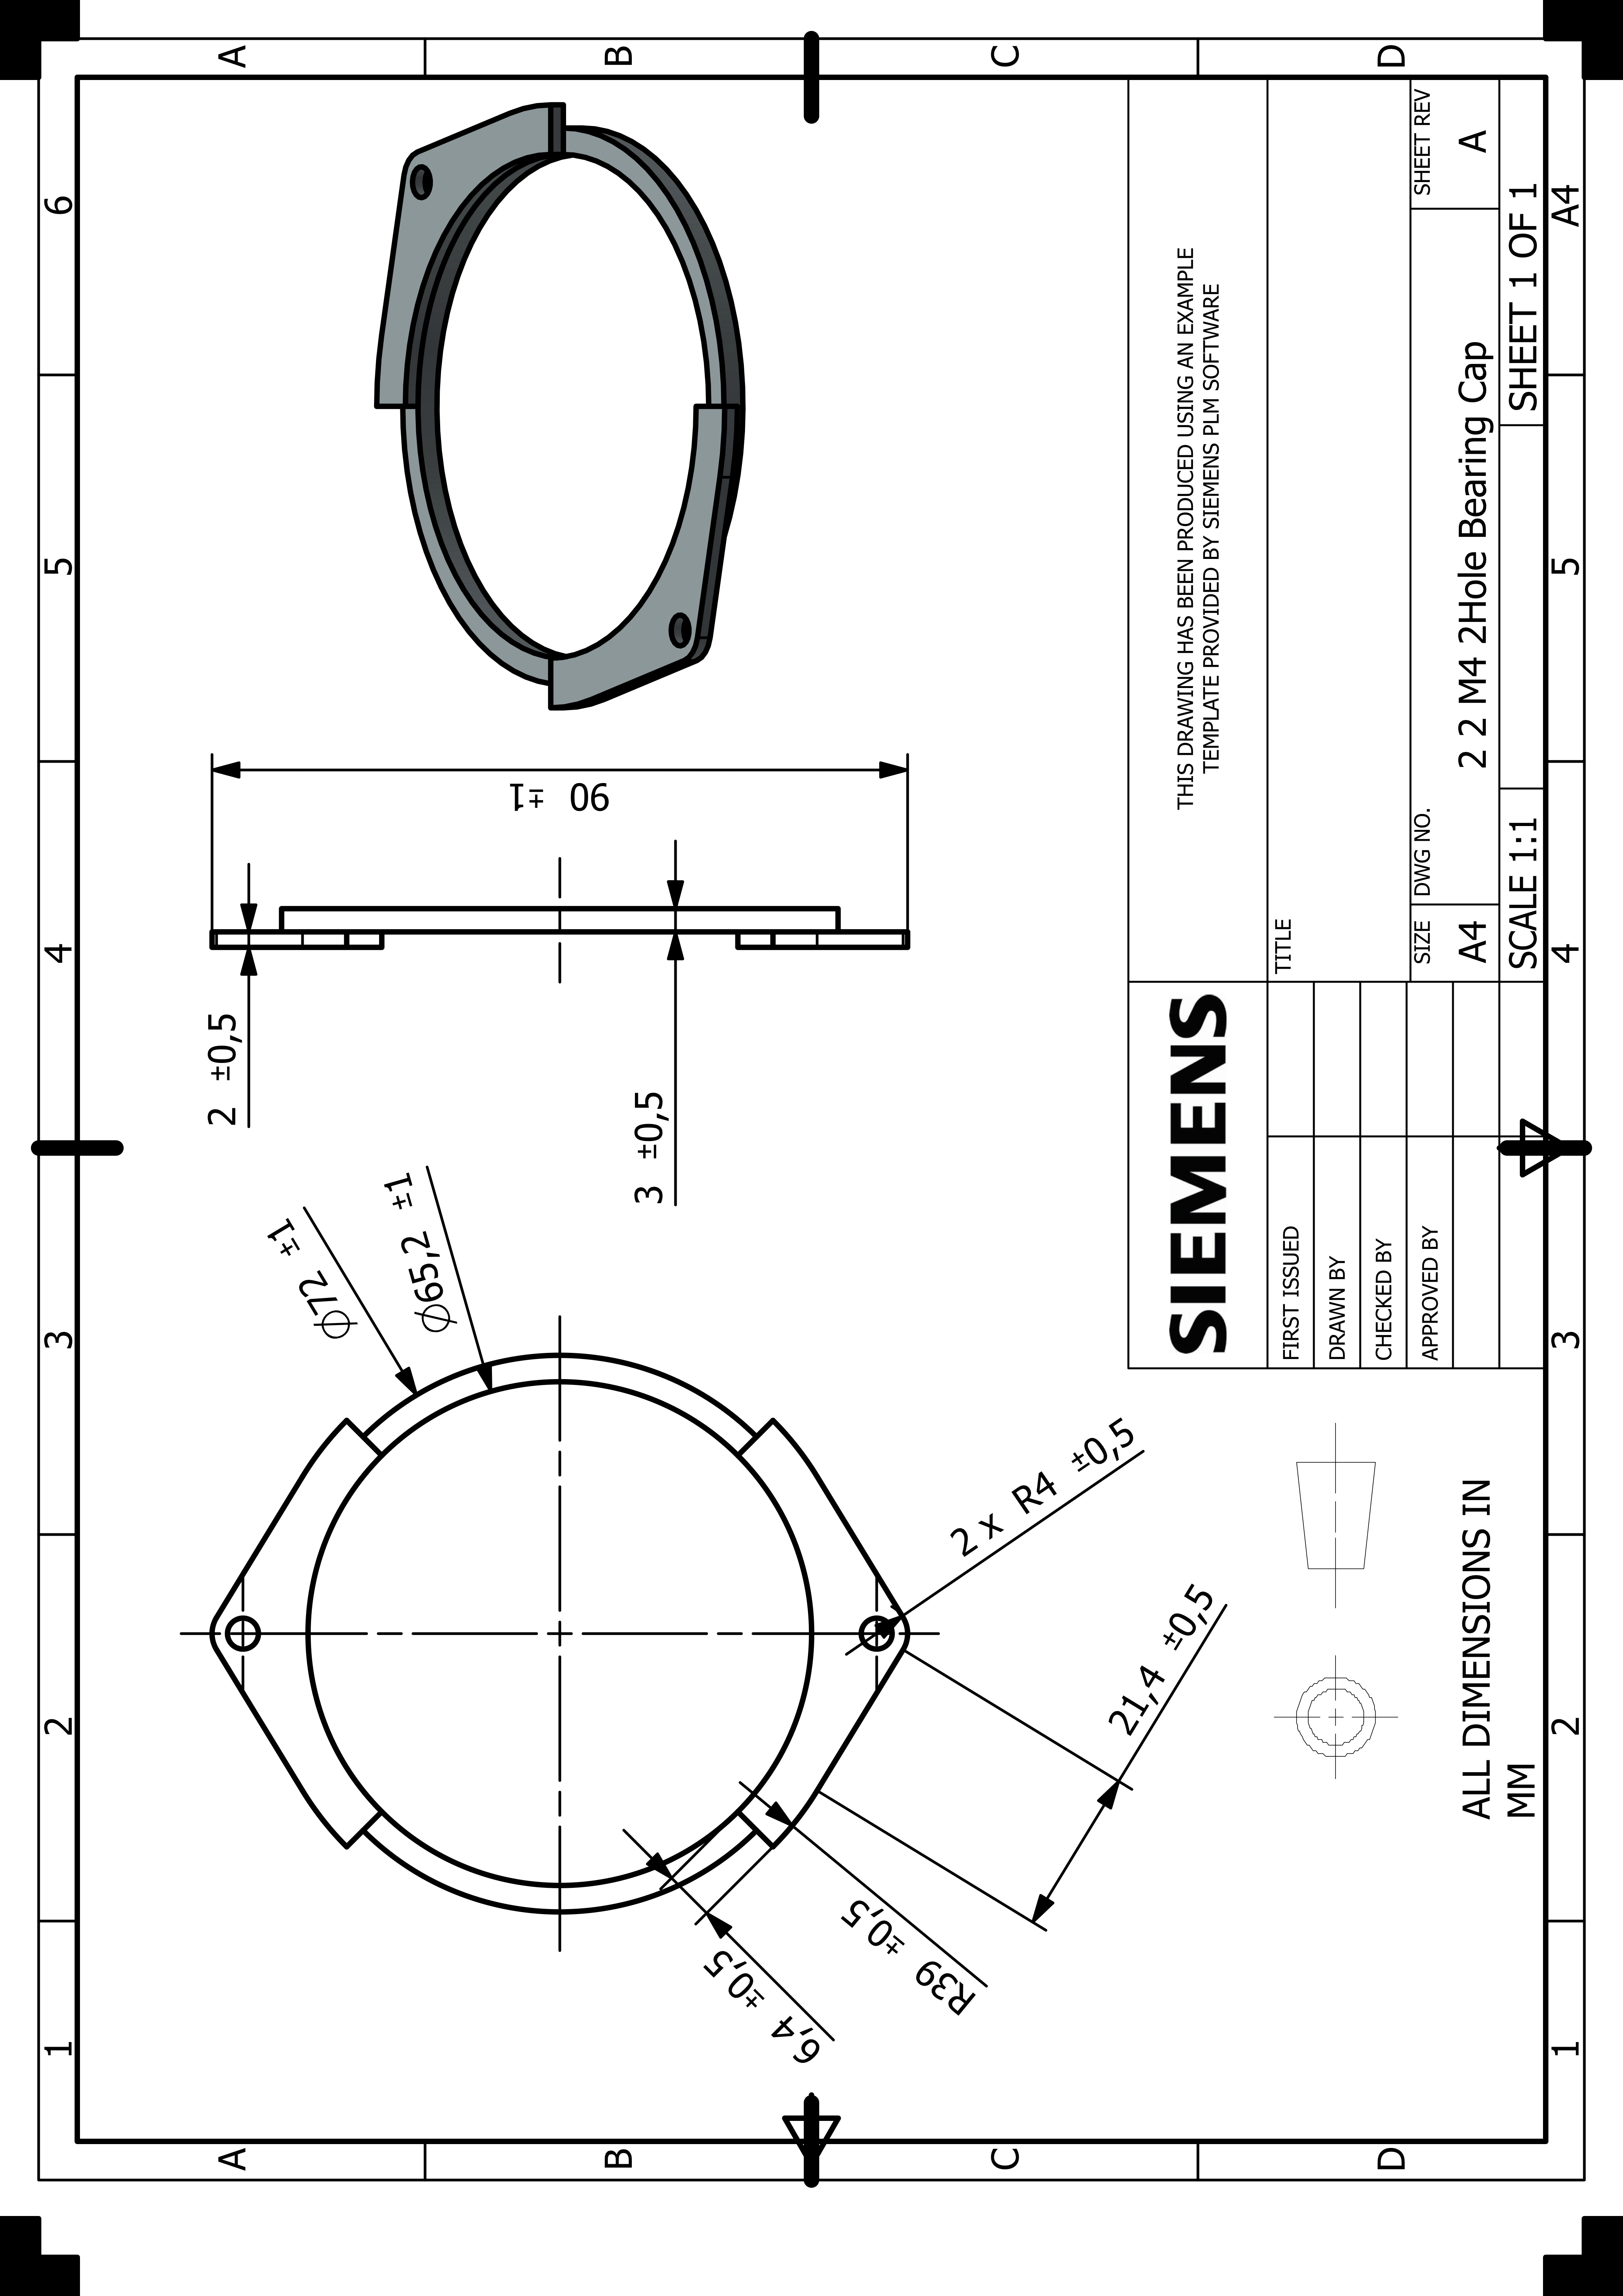
\includegraphics[width=\textwidth]{HP_2 2 M4 2Hole Bearing Cap.png} 
    \caption{Technical drawing of the hole bearing cap}
    \label{fig:technical-drawing}
\end{figure}

\begin{figure}[H]
    \centering
    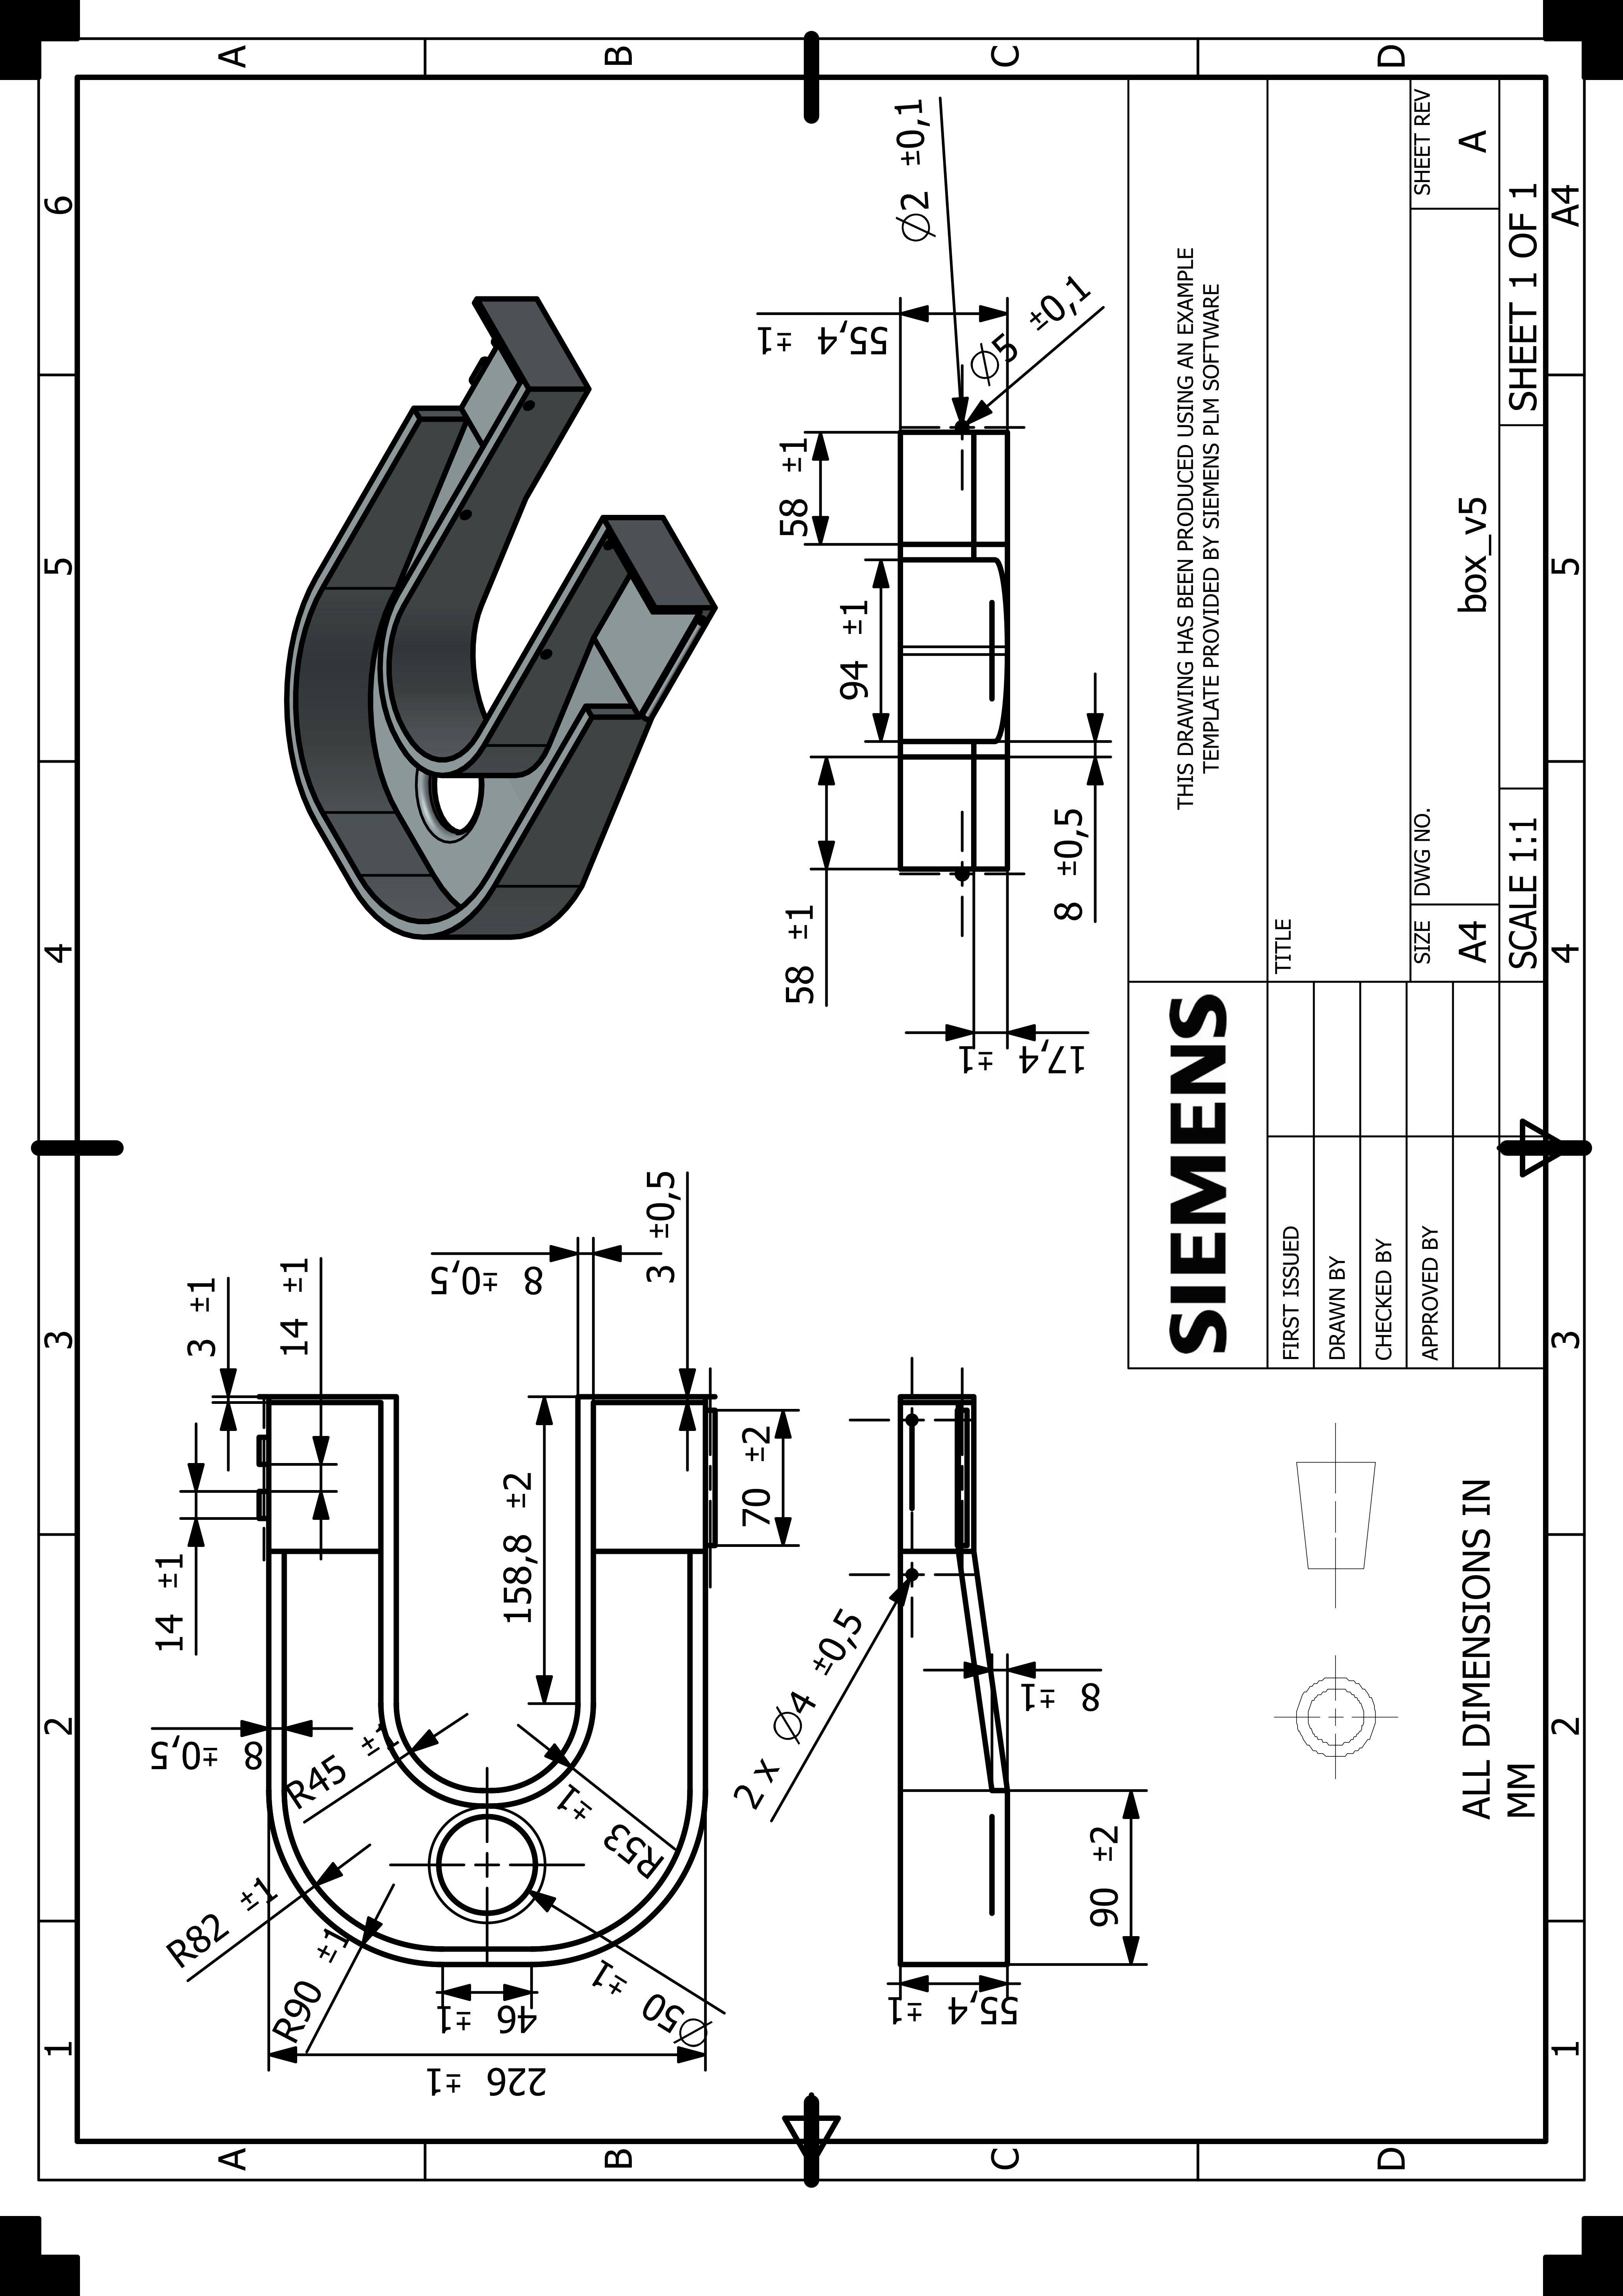
\includegraphics[width=\textwidth]{HP_box_v5.png} 
    \caption{Technical drawing of the storage}
    \label{fig:technical-drawing}
\end{figure}

\begin{figure}[H]
    \centering
    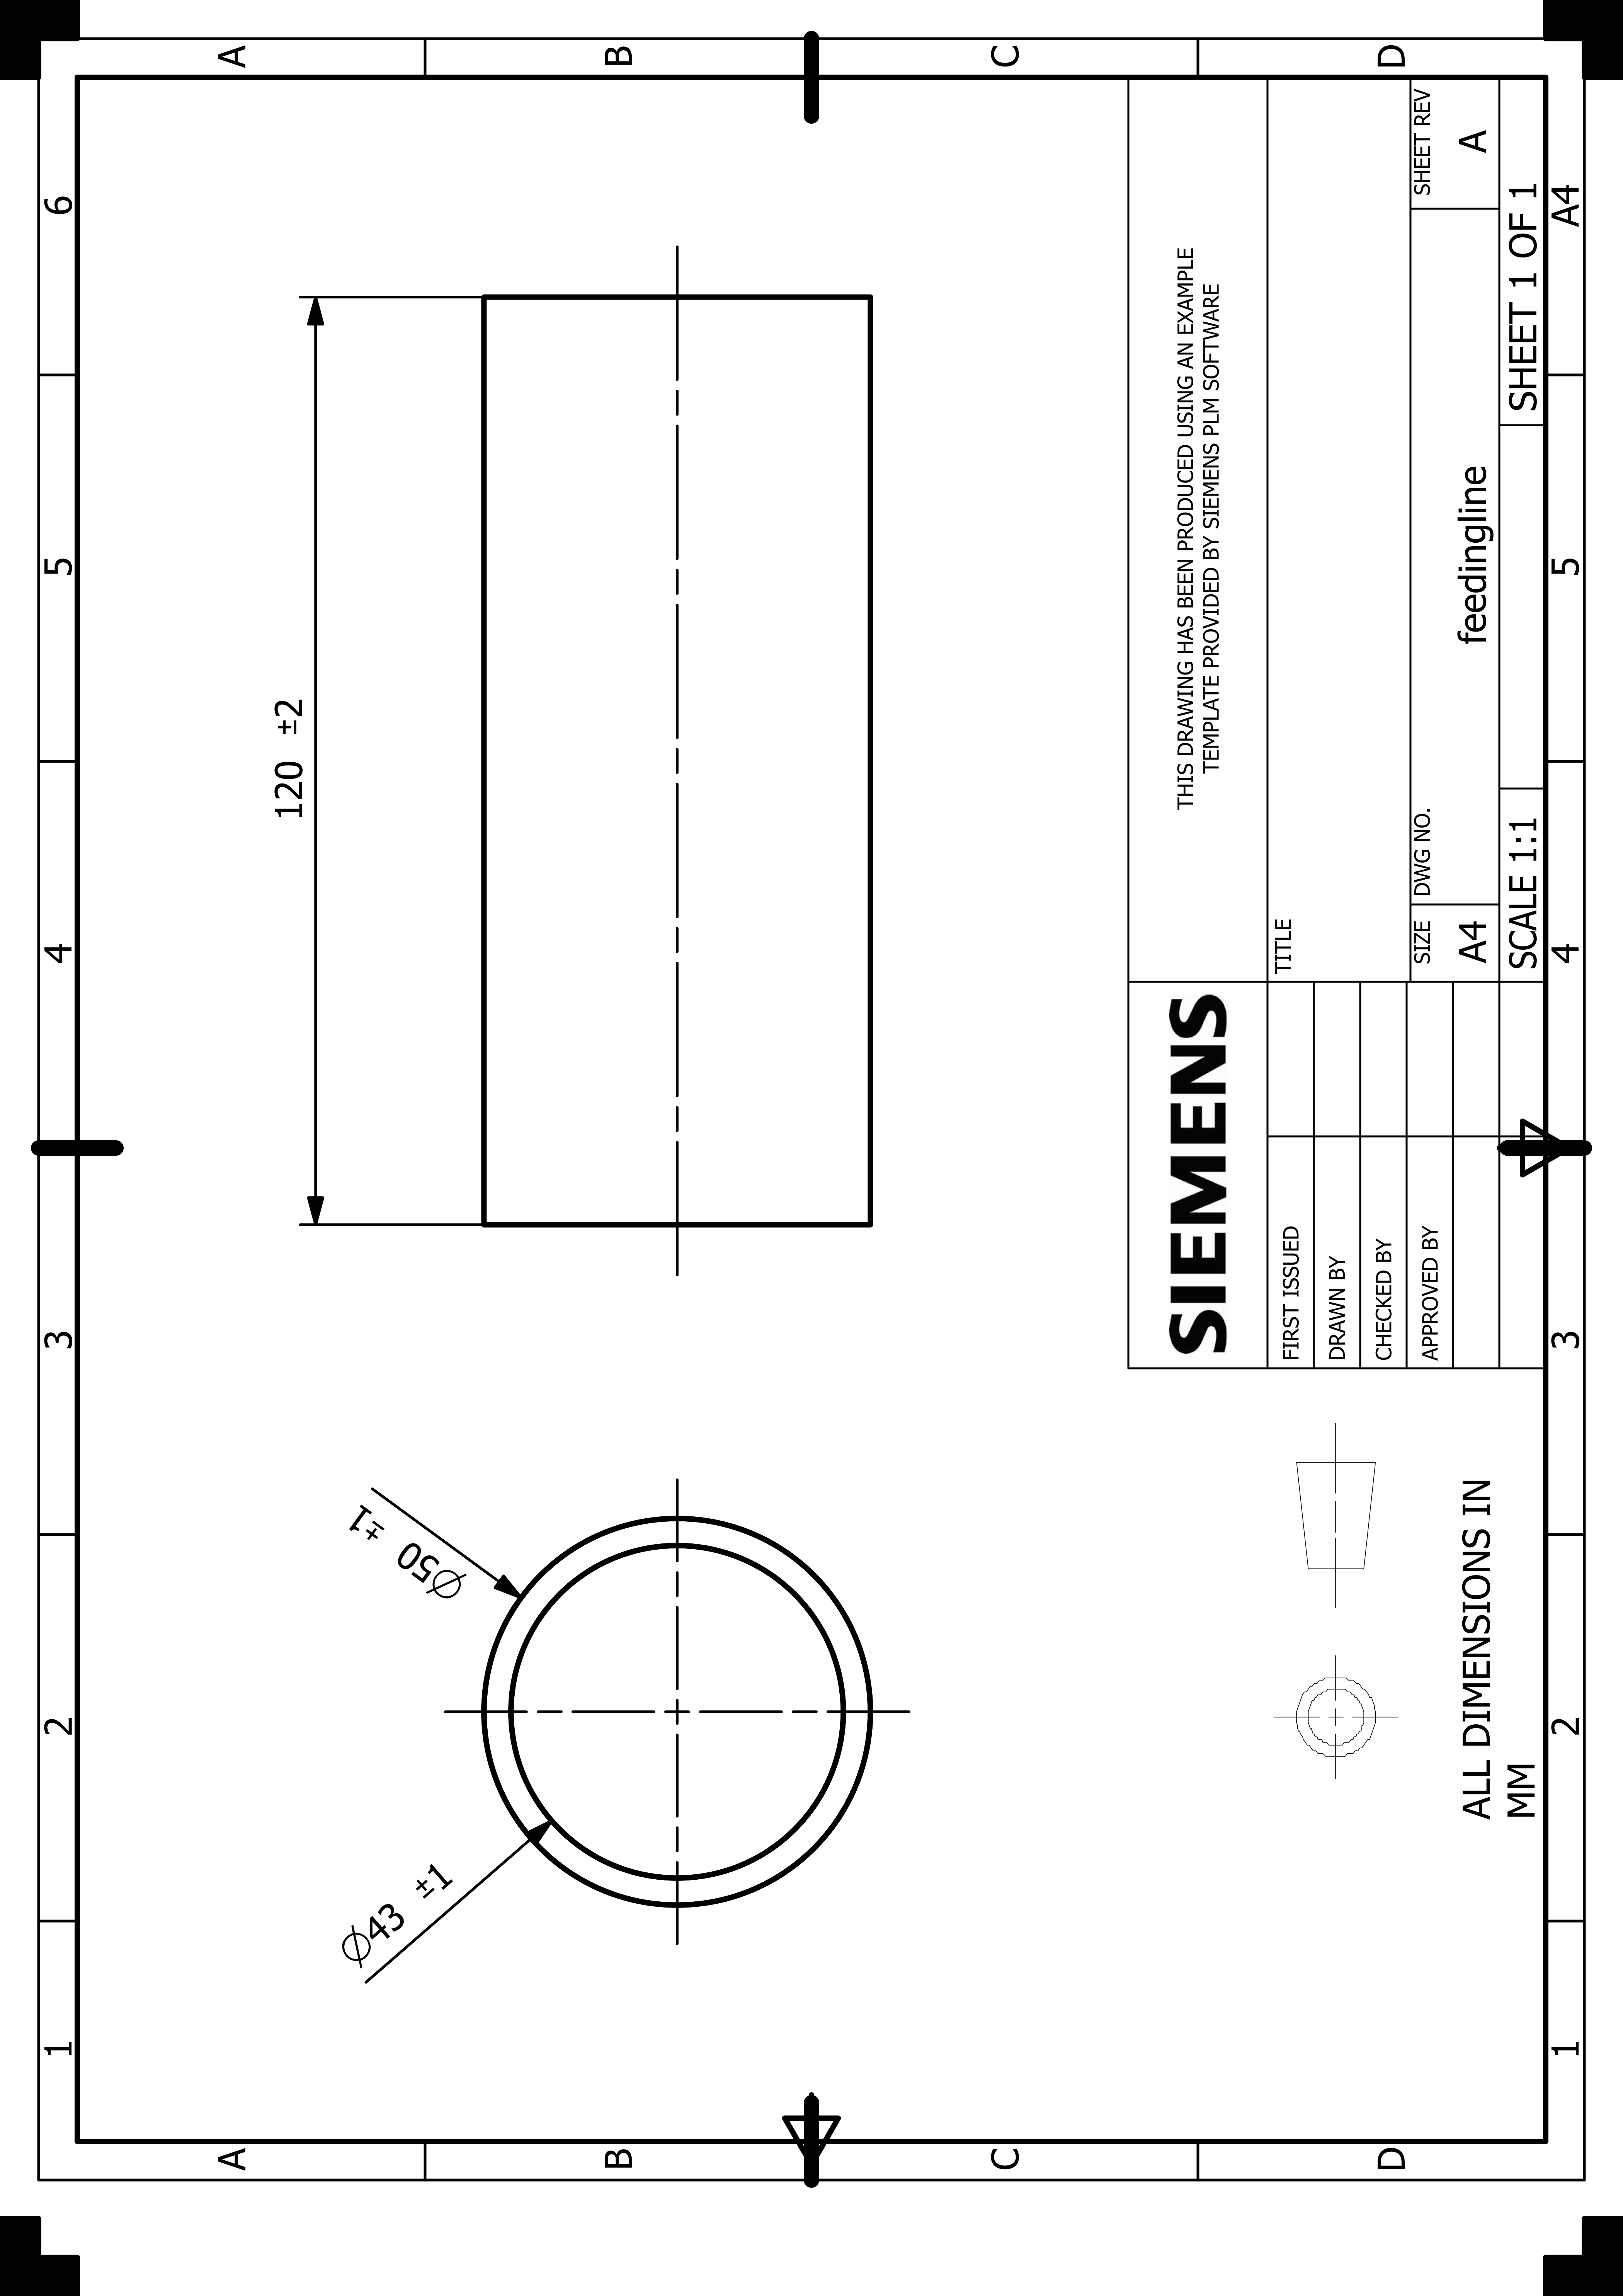
\includegraphics[width=\textwidth]{HP_feedingline.png} 
    \caption{Technical drawing of the feeding line to storage}
    \label{fig:technical-drawing}
\end{figure}

\begin{figure}[H]
    \centering
    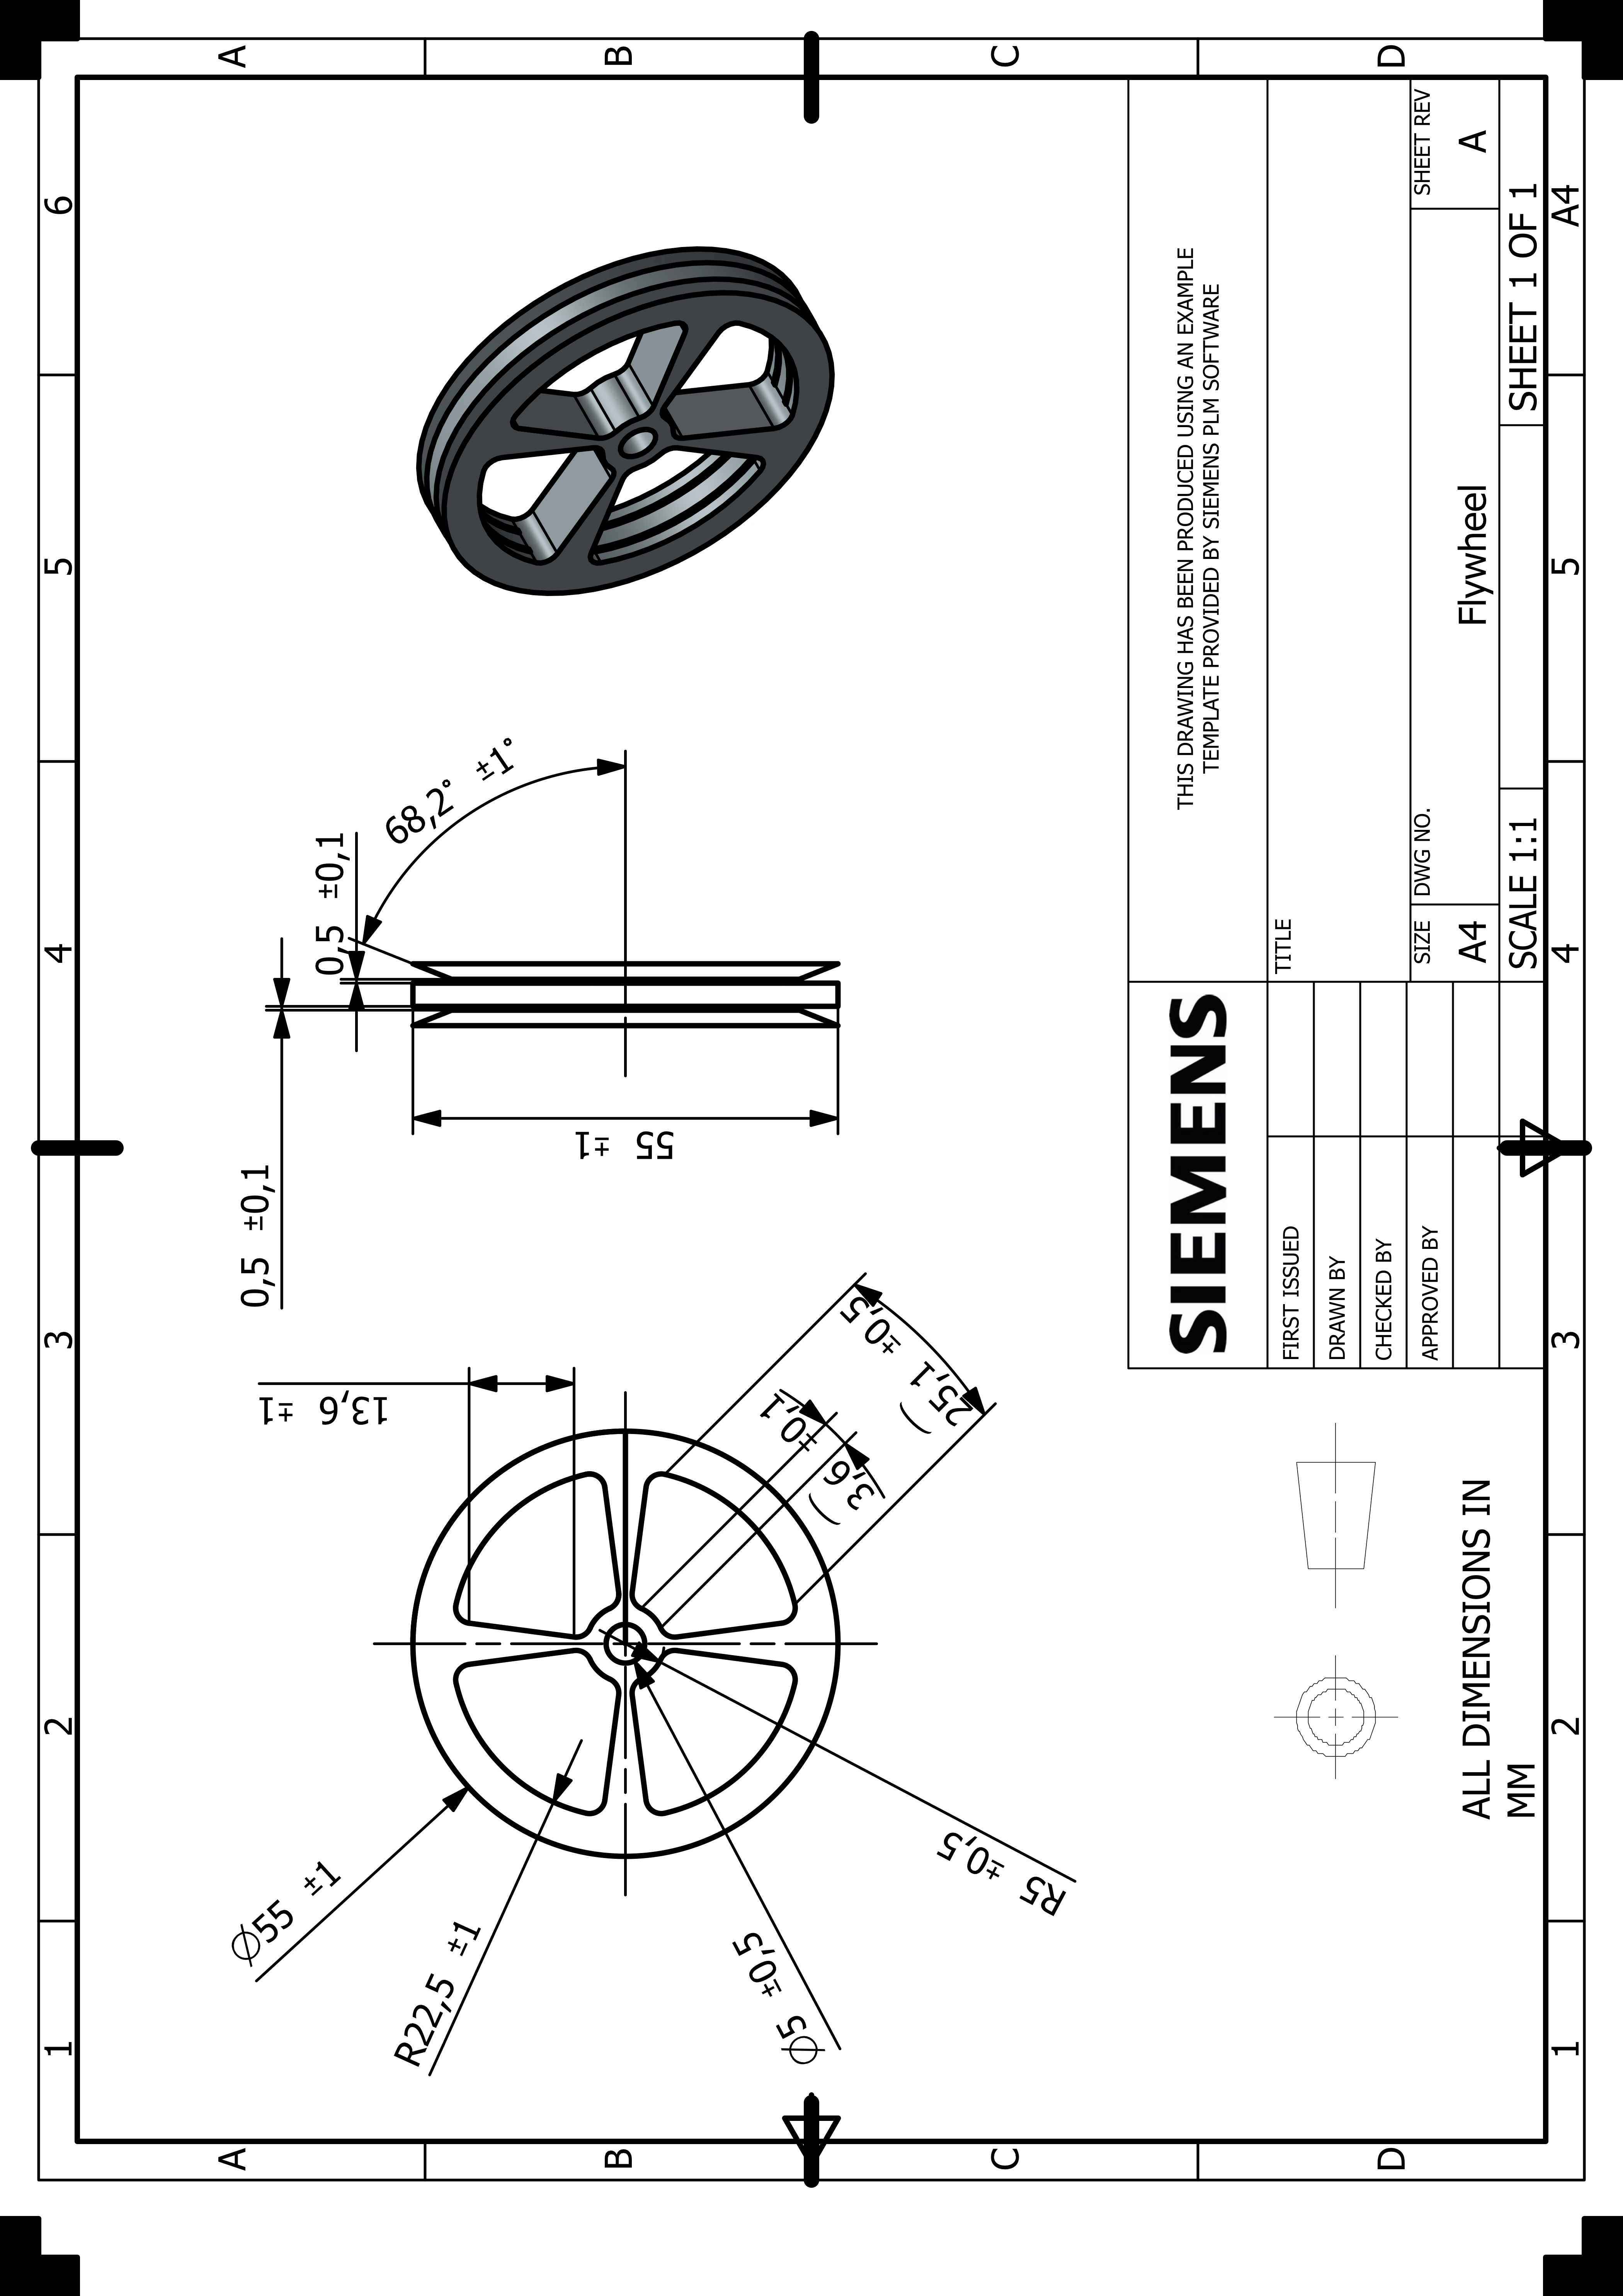
\includegraphics[width=\textwidth]{HP_Flywheel.png} 
    \caption{Technical drawing of the flywheel}
    \label{fig:technical-drawing}
\end{figure}

\begin{figure}[H]
    \centering
    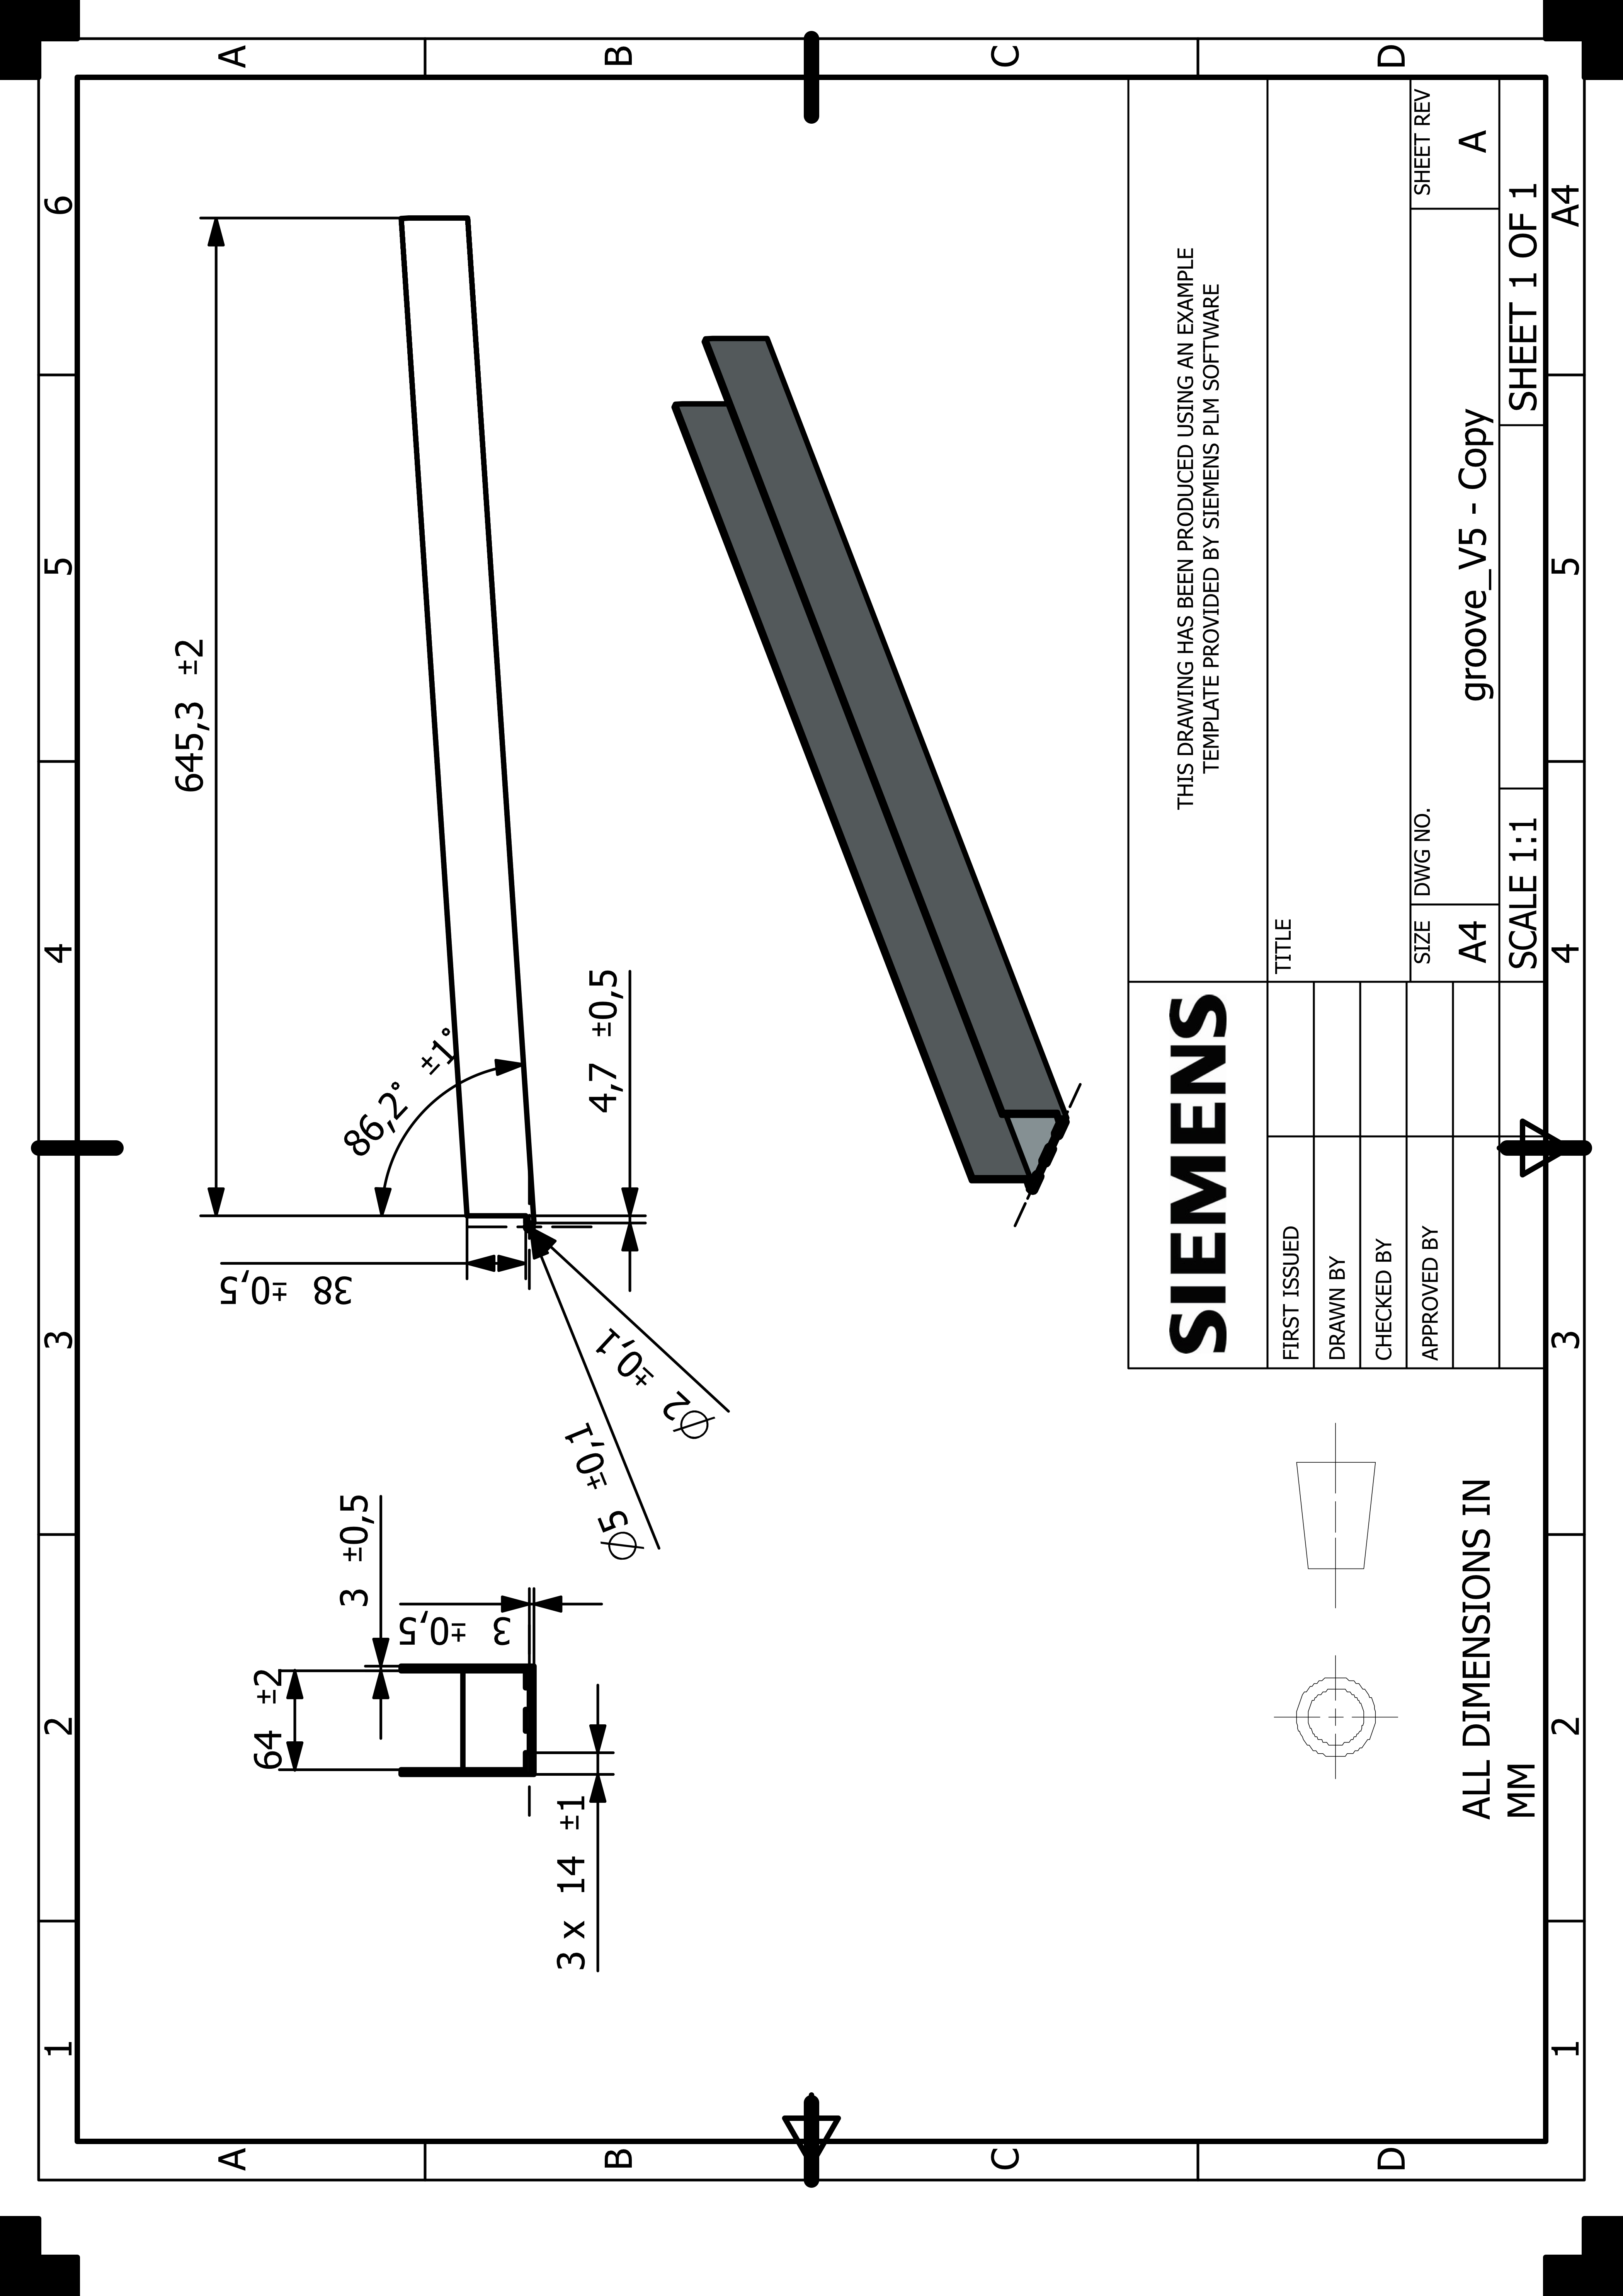
\includegraphics[width=\textwidth]{HP_groove_V5 - Copy.png} 
    \caption{Technical drawing of the groove}
    \label{fig:technical-drawing}
\end{figure}

\begin{figure}[H]
    \centering
    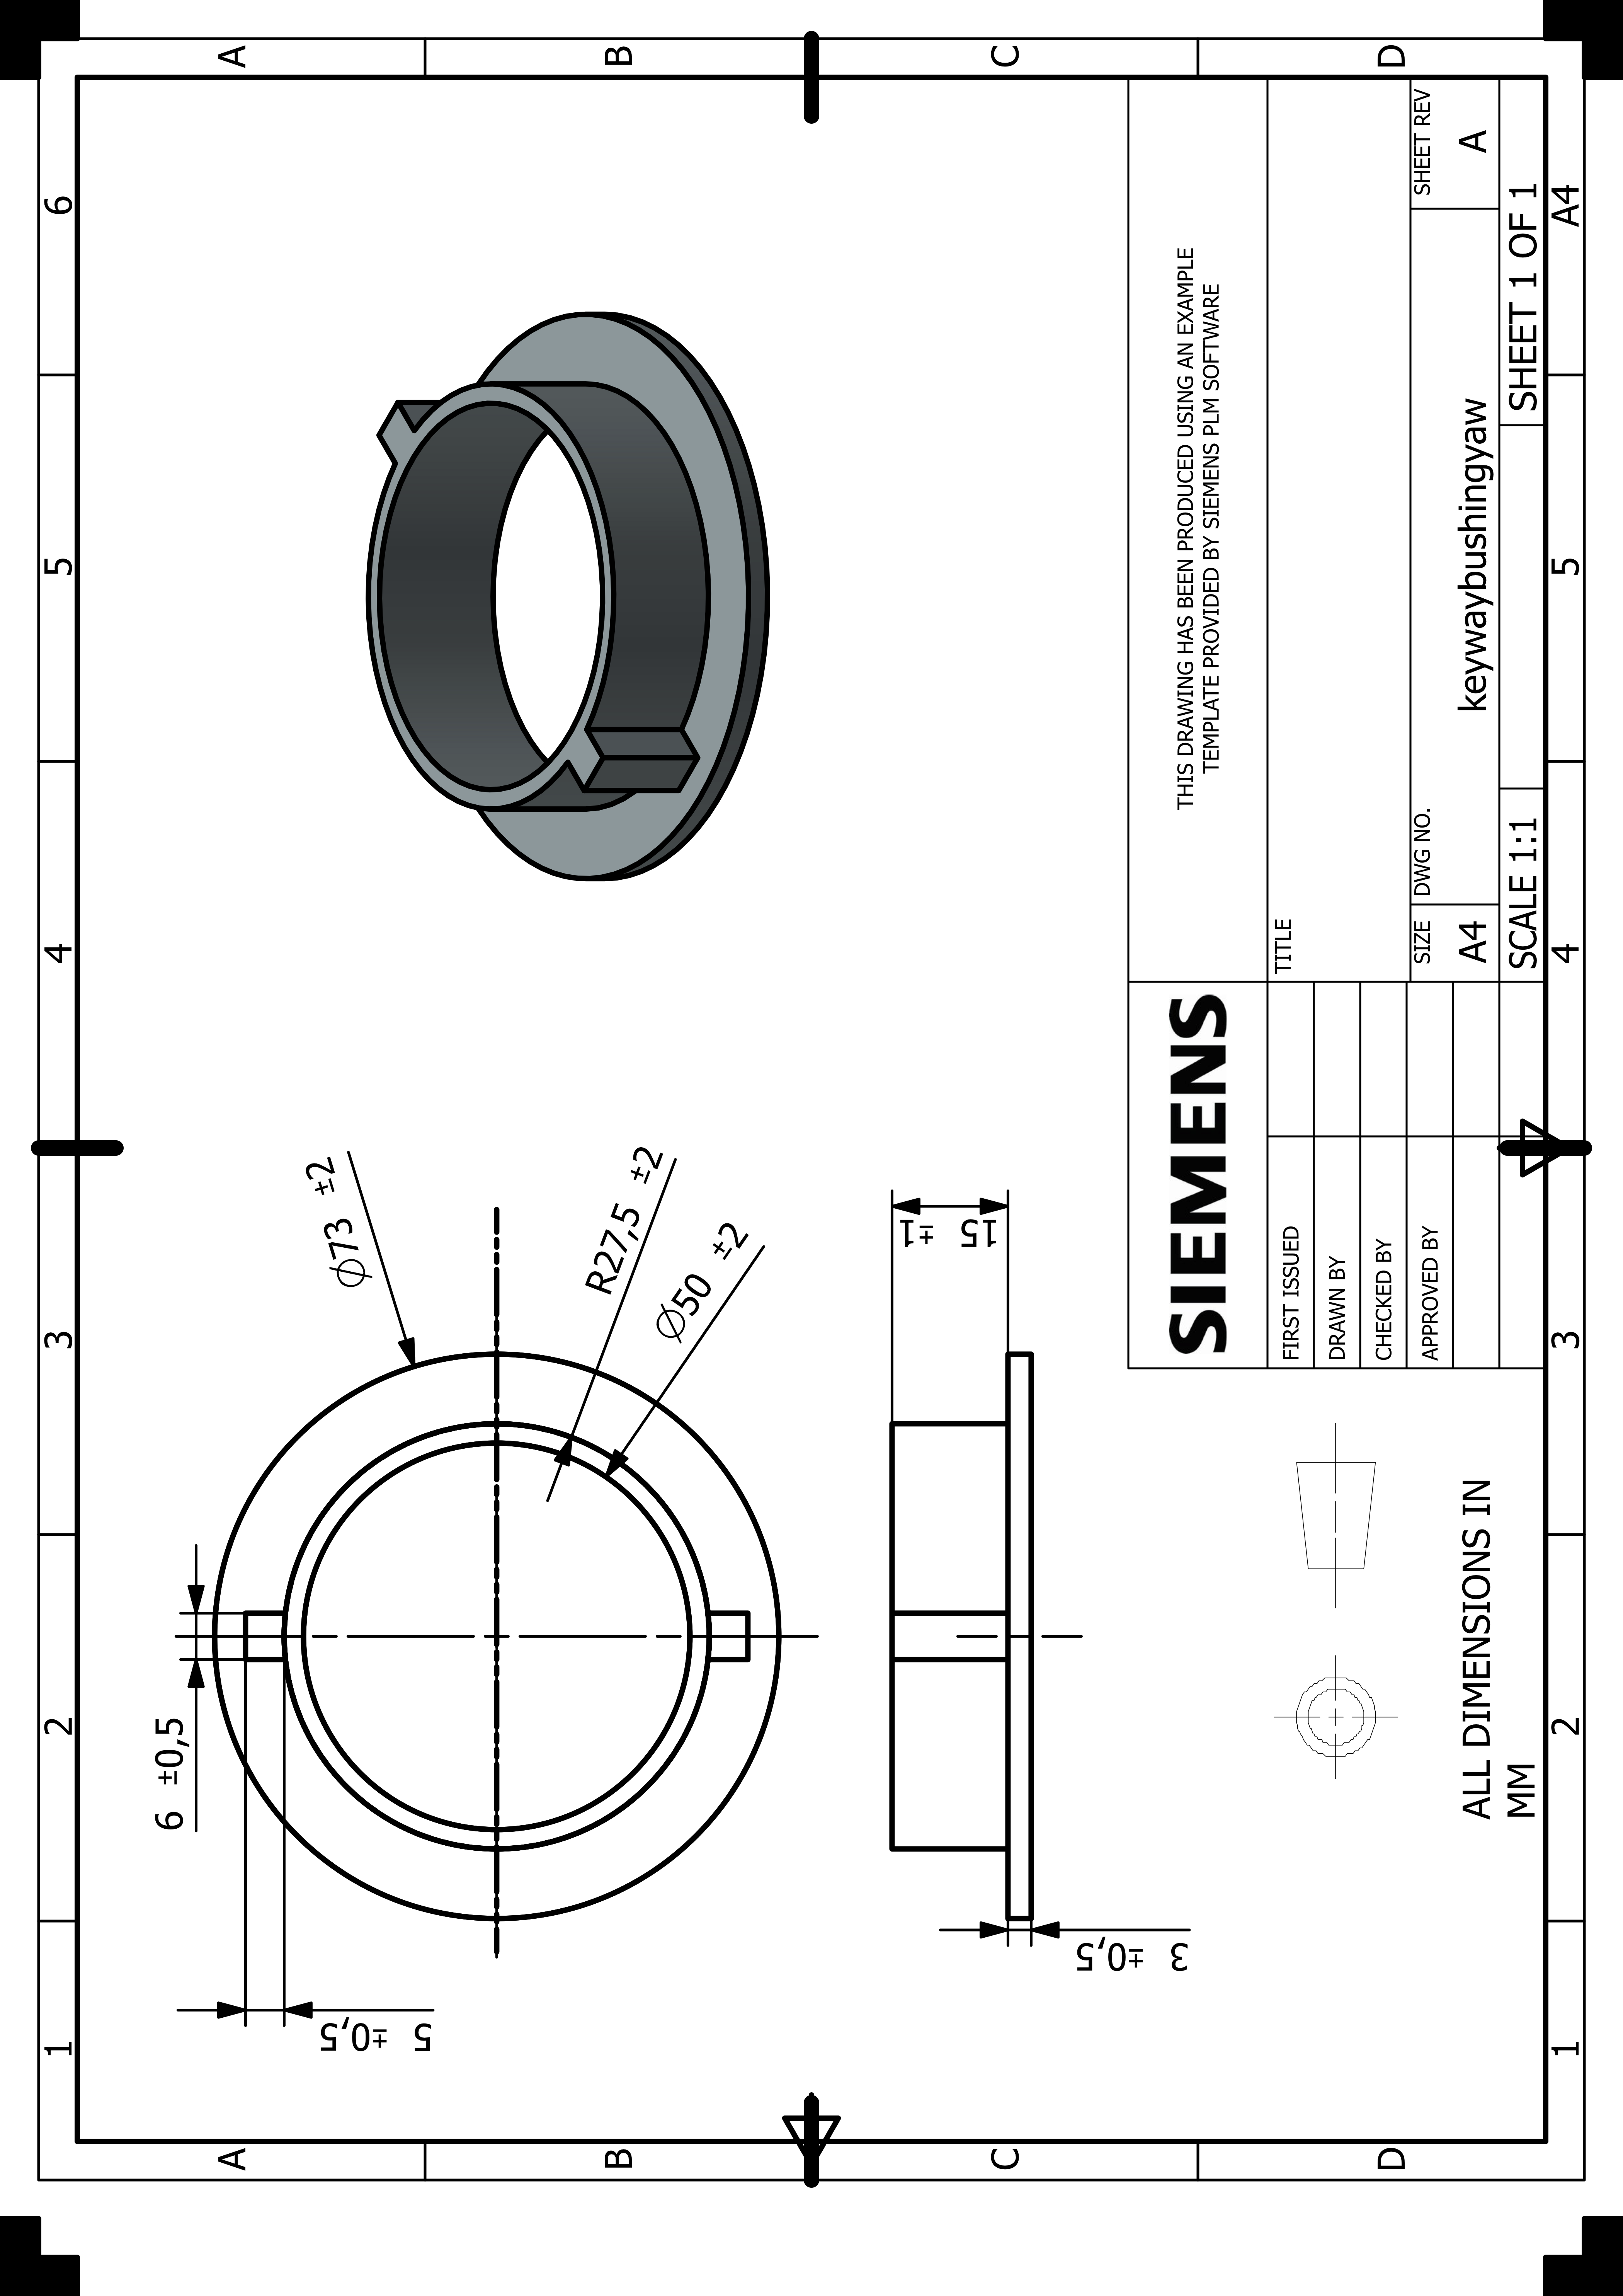
\includegraphics[width=\textwidth]{HP_keywaybushingyaw.png} 
    \caption{Technical drawing of the keyway bushing for yaw mechanism}
    \label{fig:technical-drawing}
\end{figure}

\begin{figure}[H]
    \centering
    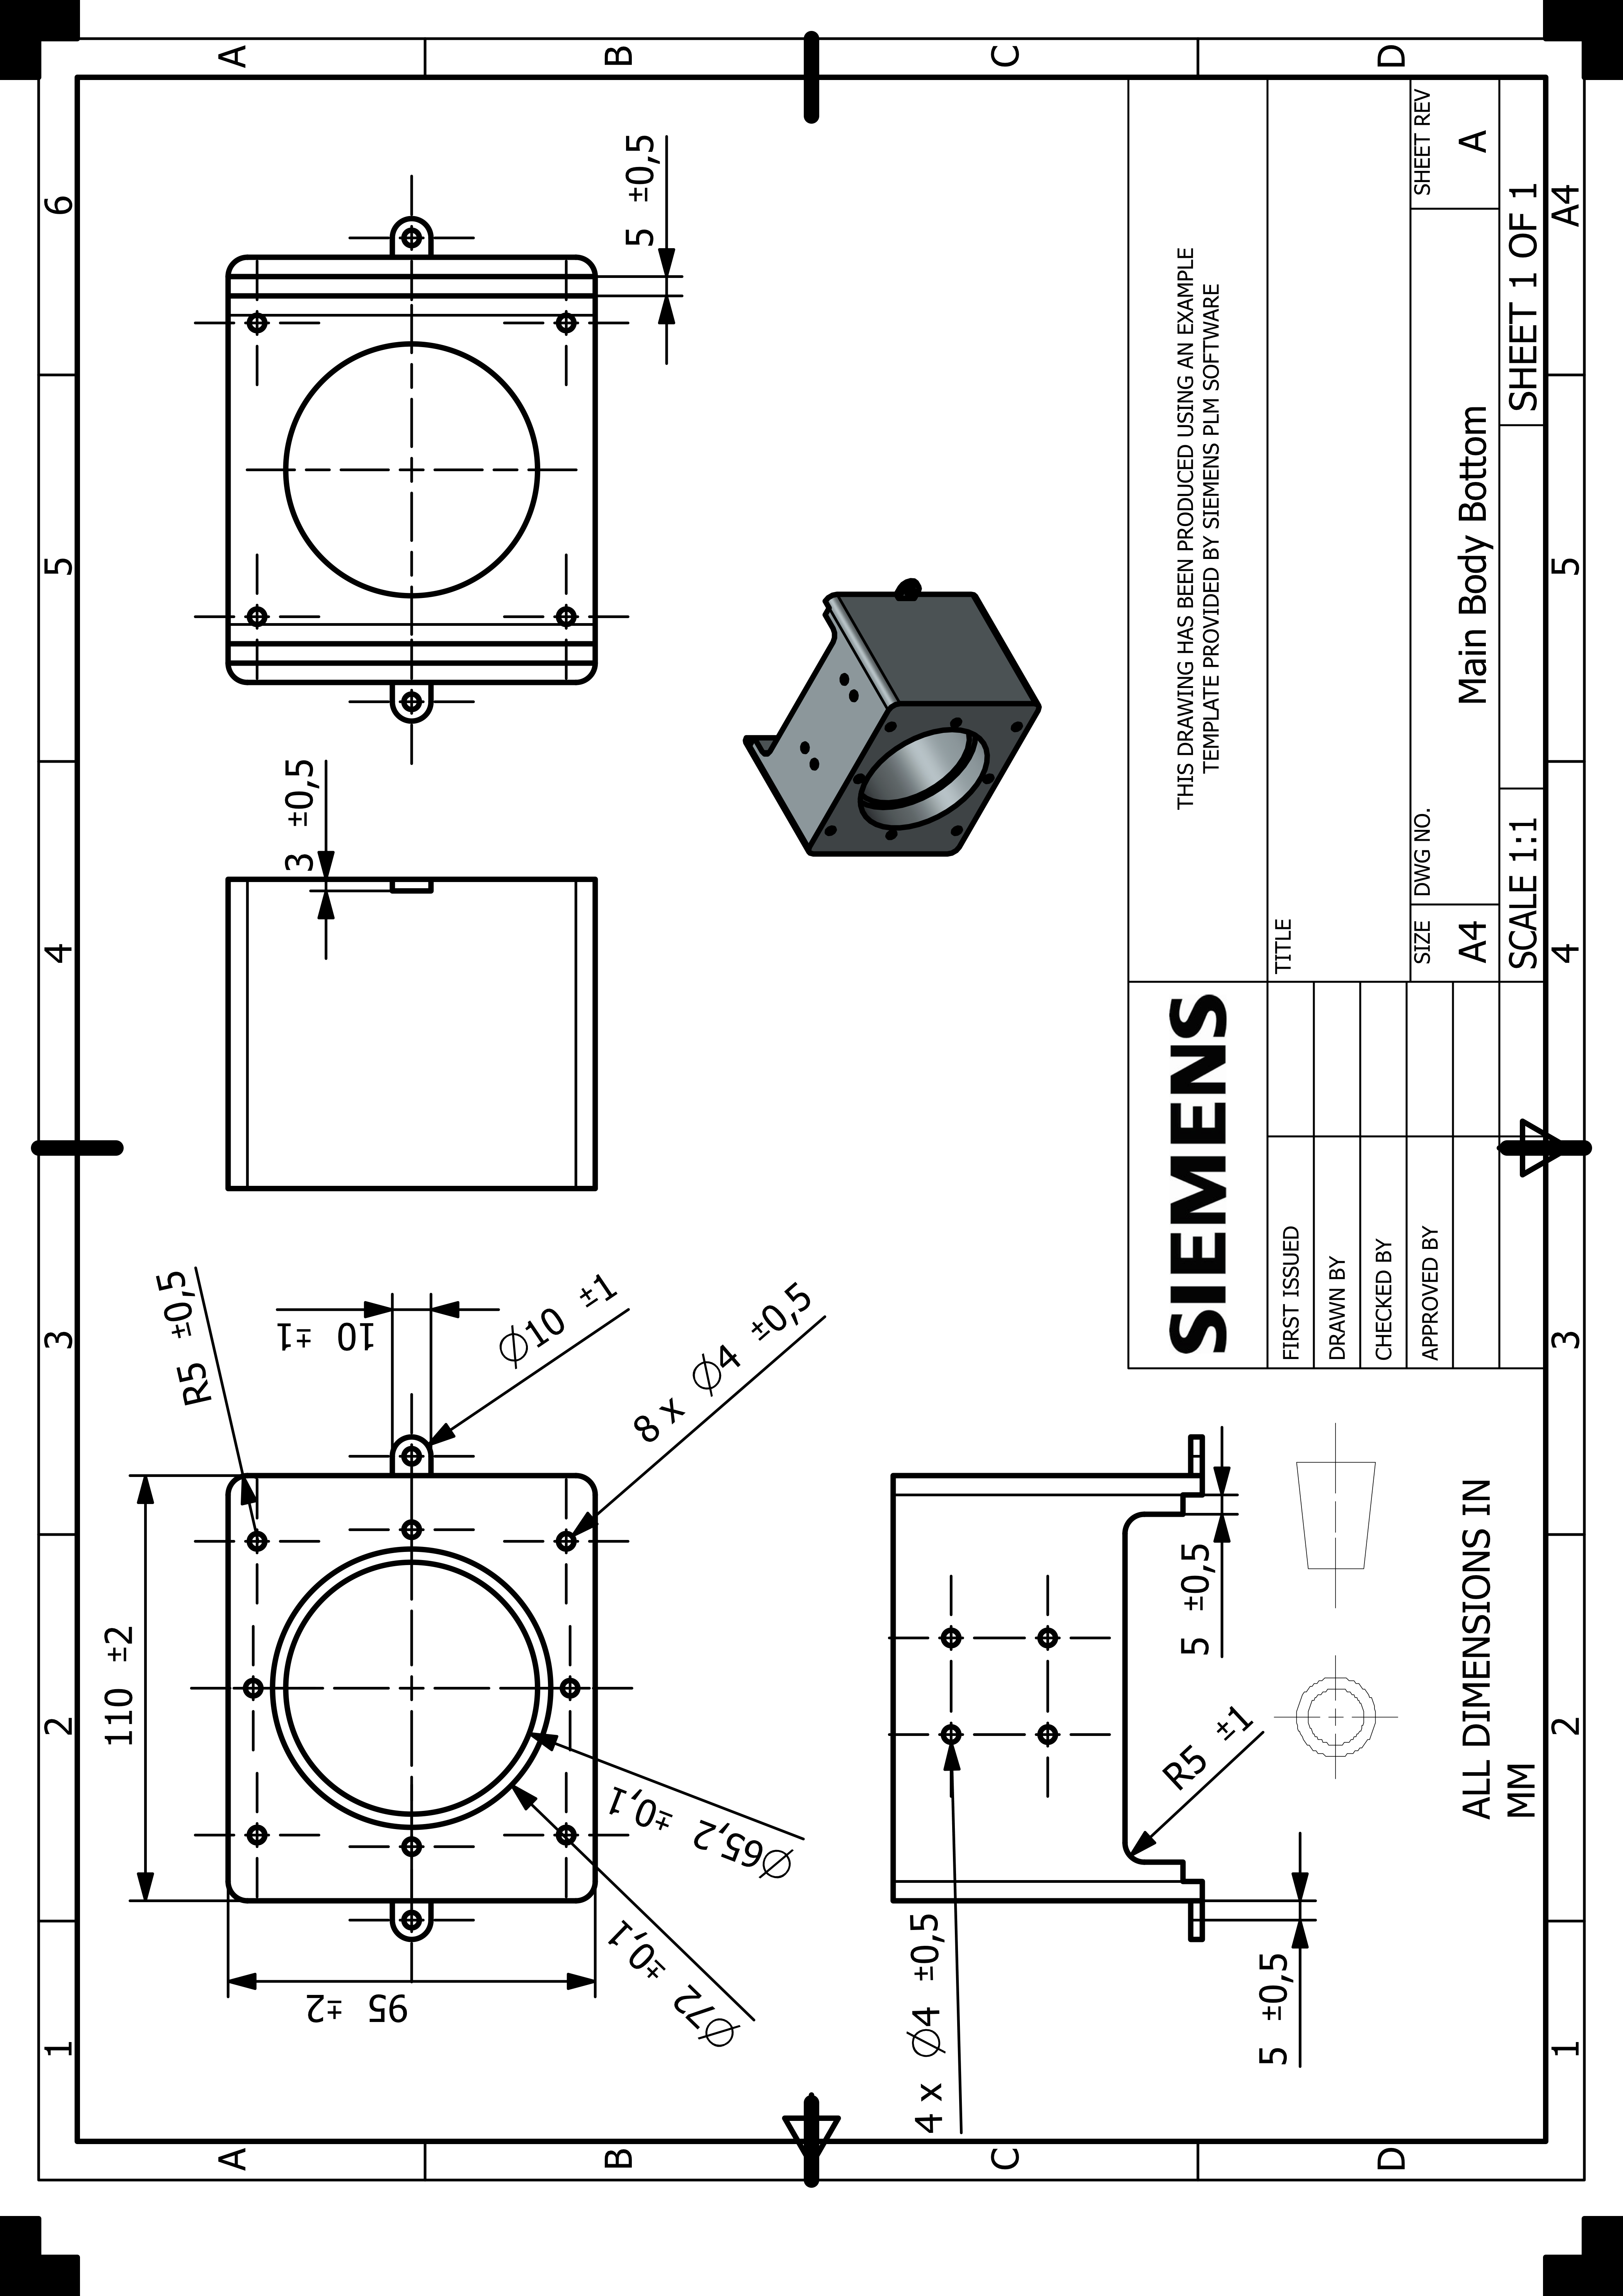
\includegraphics[width=\textwidth]{HP_Main Body Bottom.png} 
    \caption{Technical drawing of the bottom part of the main body}
    \label{fig:technical-drawing}
\end{figure}

\begin{figure}[H]
    \centering
    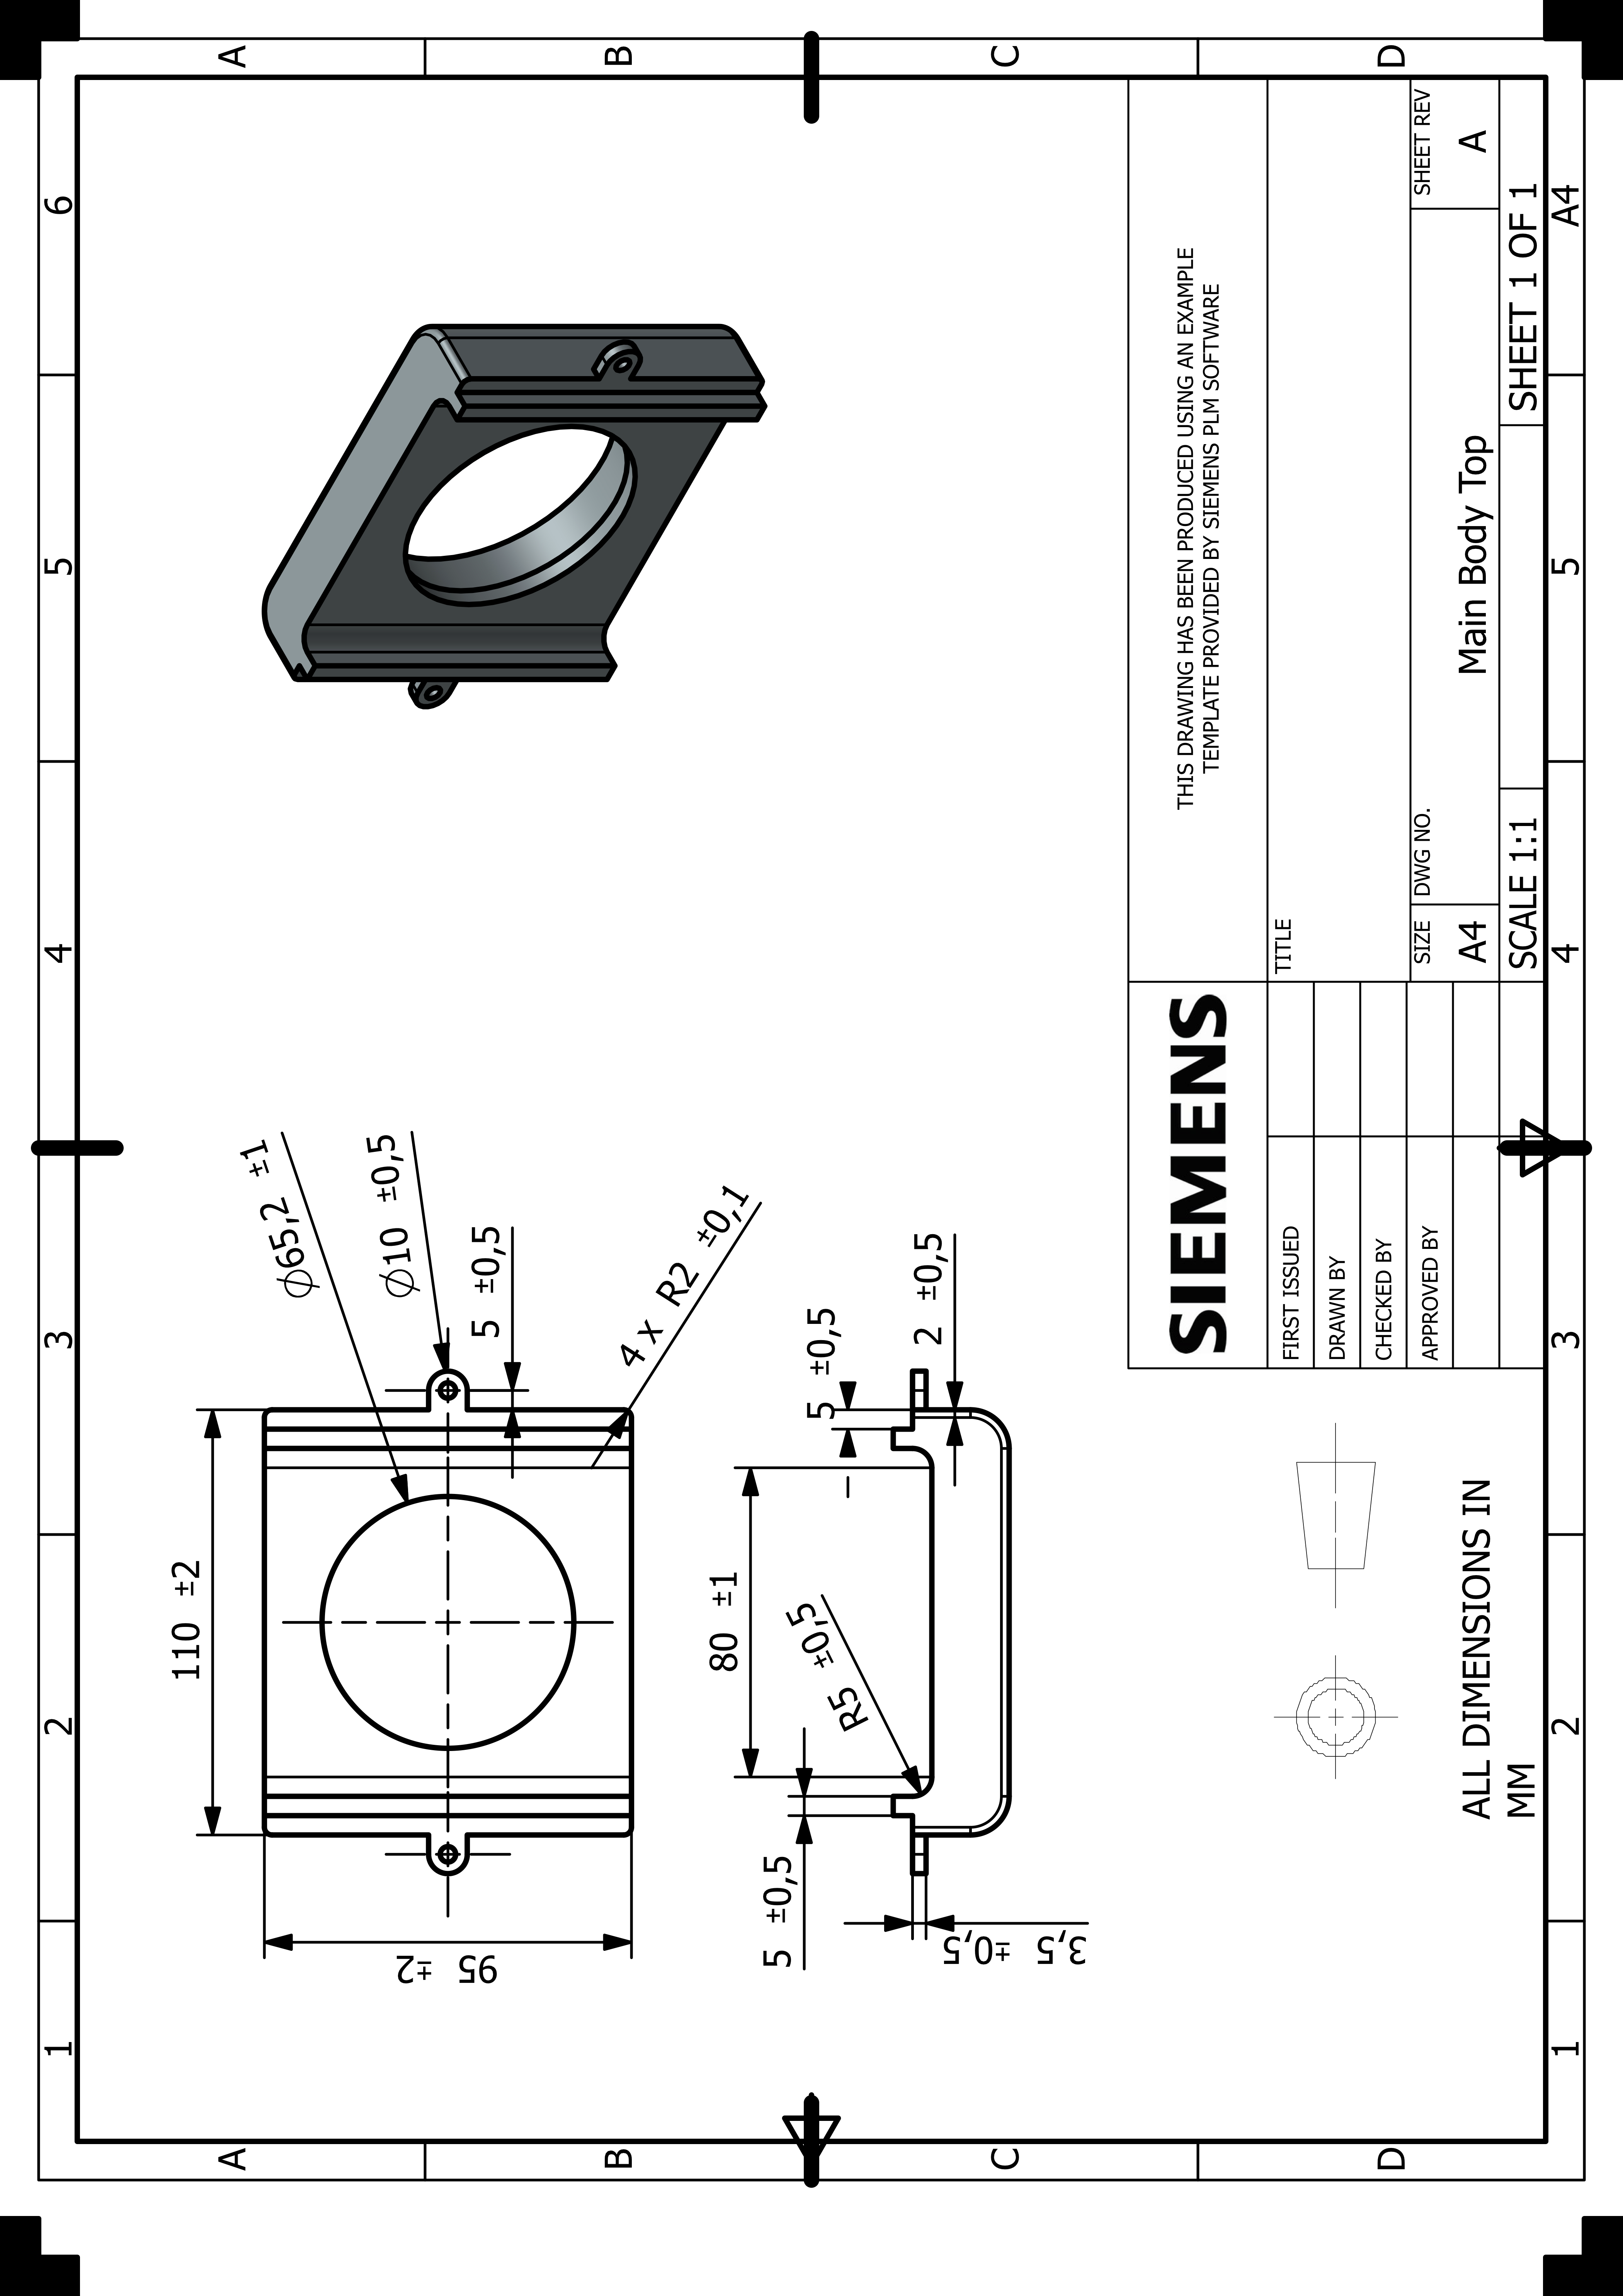
\includegraphics[width=\textwidth]{HP_Main Body Top.png} 
    \caption{Technical drawing of the upper part of the main body}
    \label{fig:technical-drawing}
\end{figure}

\begin{figure}[H]
    \centering
    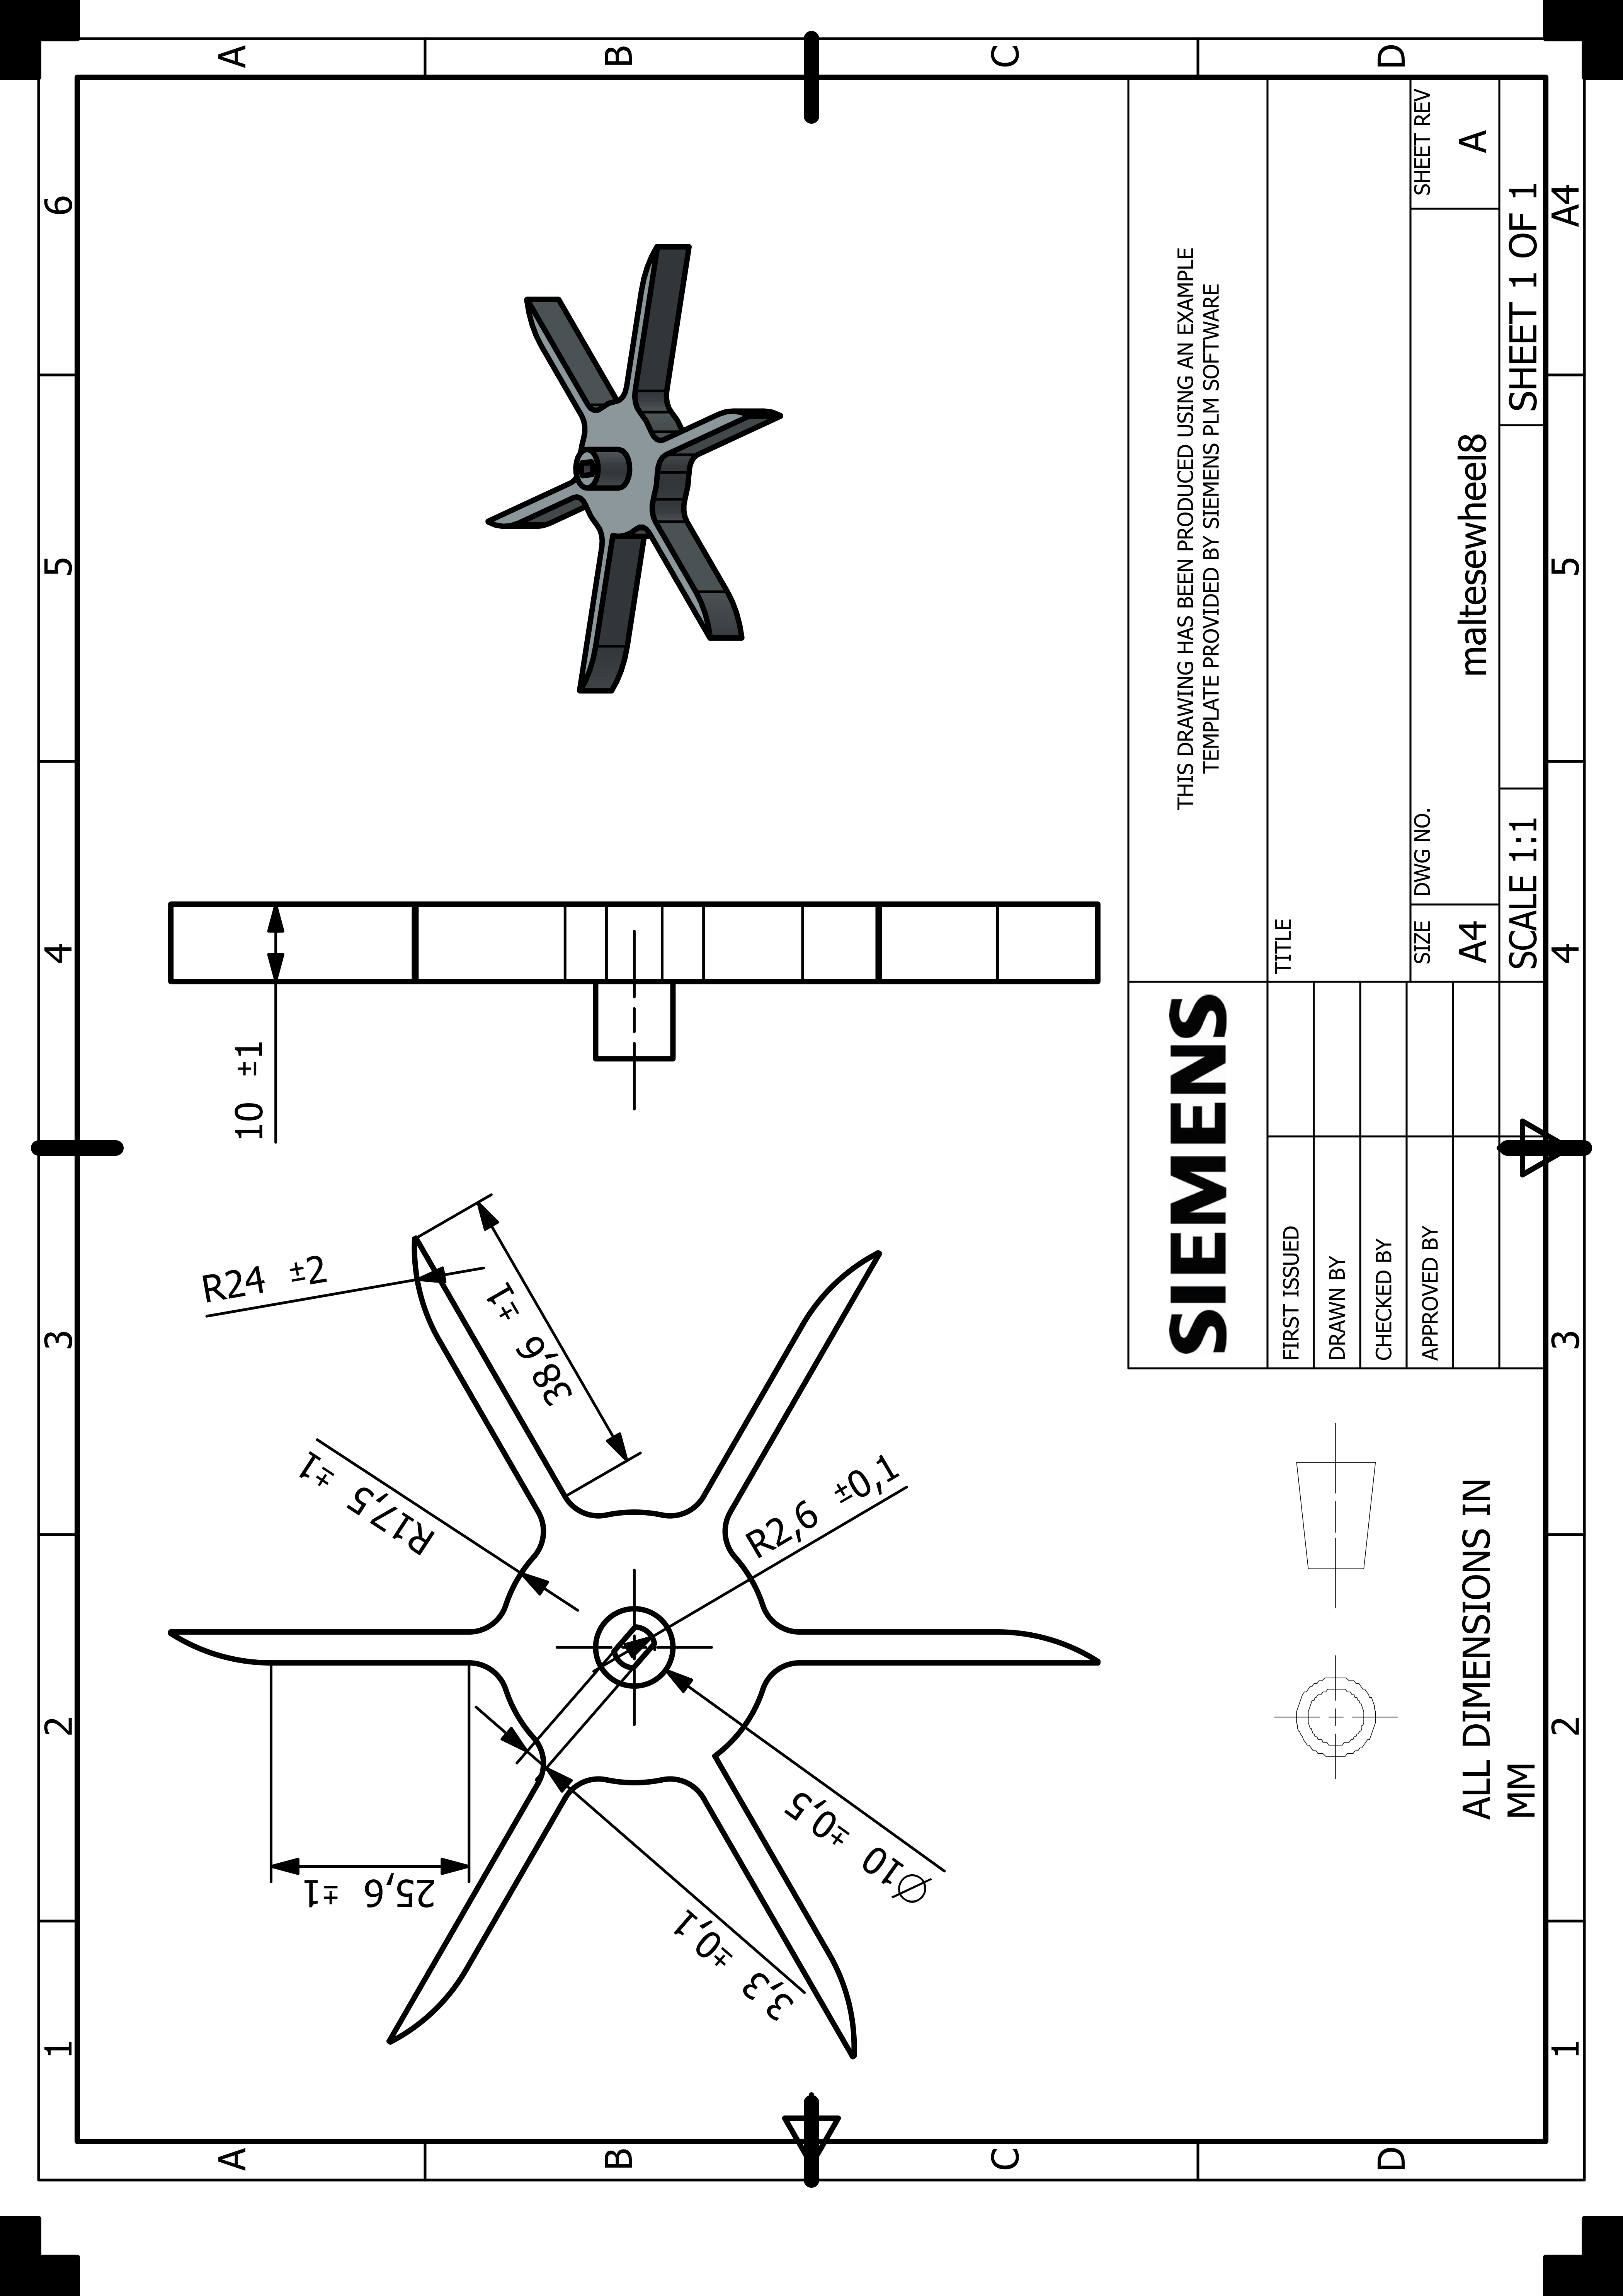
\includegraphics[width=\textwidth]{HP_maltesewheel8.png} 
    \caption{Technical drawing of the Maltese wheel}
    \label{fig:technical-drawing}
\end{figure}

\begin{figure}[H]
    \centering
    \includegraphics[width=\textwidth]{özge_slotted pipe.png} 
    \caption{Technical drawing of the slotted pipe for the launcher head}
    \label{fig:technical-drawing}
\end{figure}

\begin{figure}[H]
    \centering
    \includegraphics[width=\textwidth]{özge_pipe_attachment.png} 
    \caption{Technical drawing of the pipe attachment for launcher head}
    \label{fig:technical-drawing}
\end{figure}

\begin{figure}[H]
    \centering
    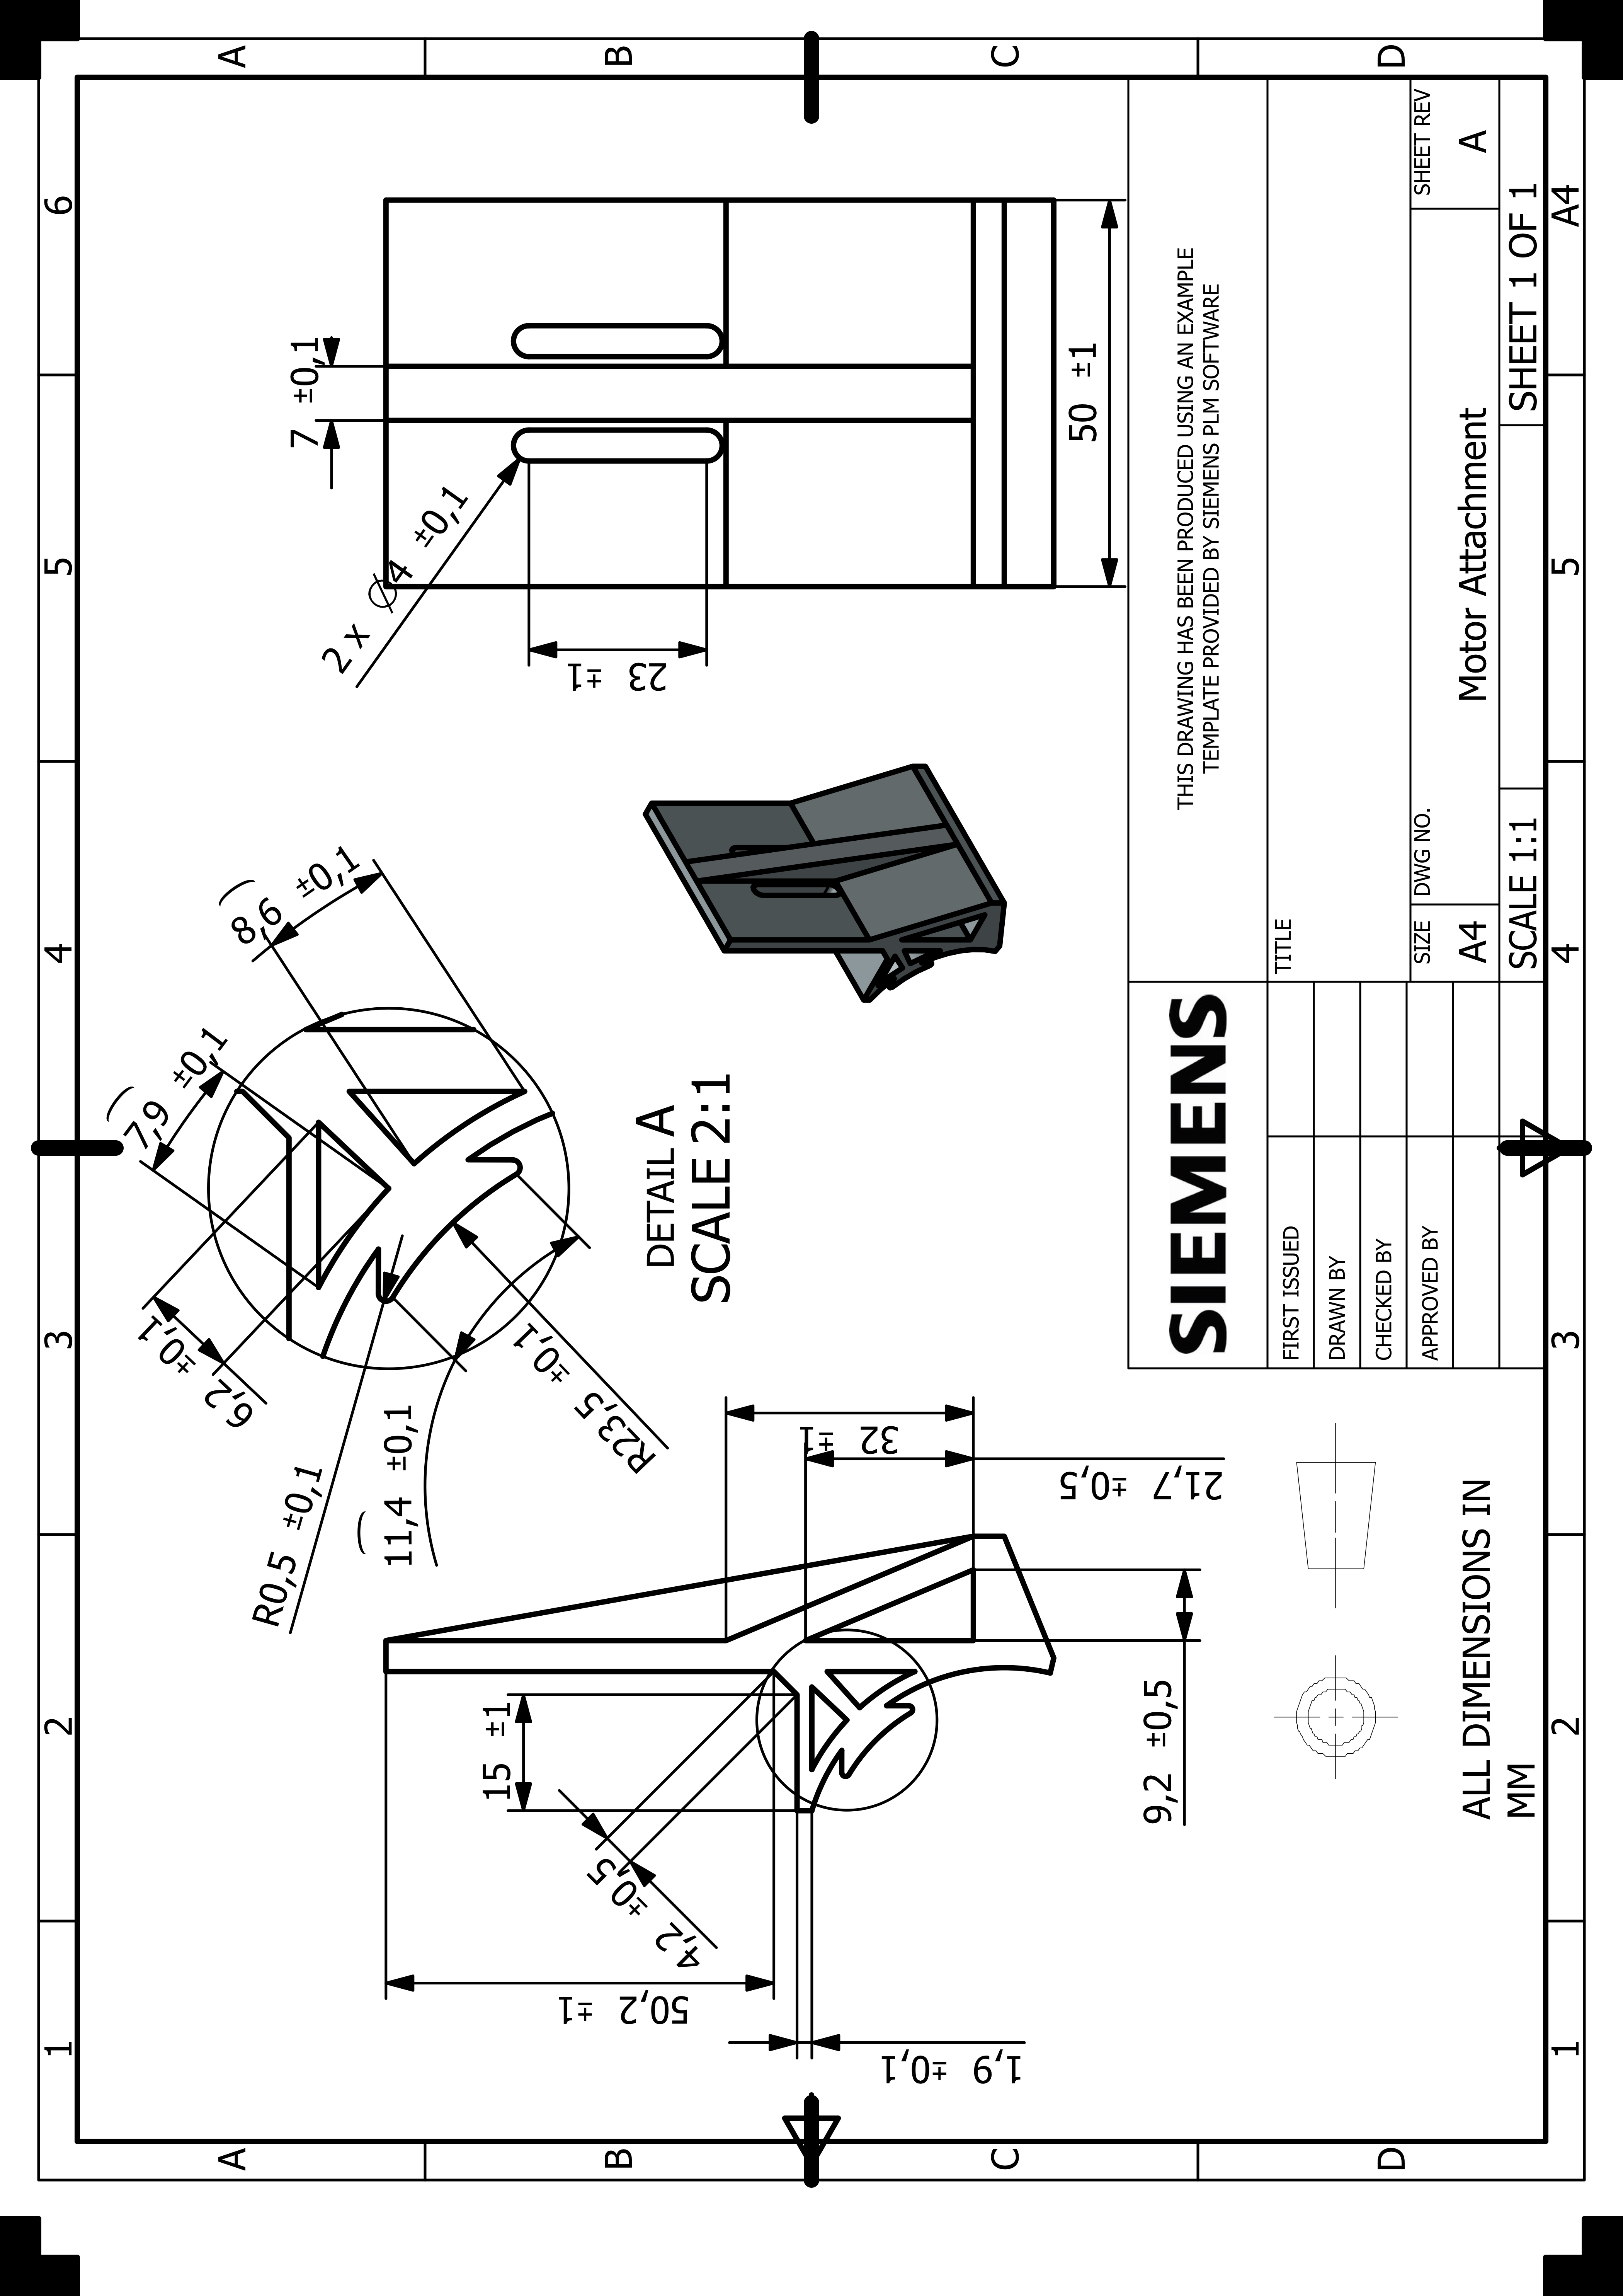
\includegraphics[width=\textwidth]{HP_Motor Attachment.png} 
    \caption{Technical drawing of the motor attachment for the launcher head}
    \label{fig:technical-drawing}
\end{figure}

\begin{figure}[H]
    \centering
    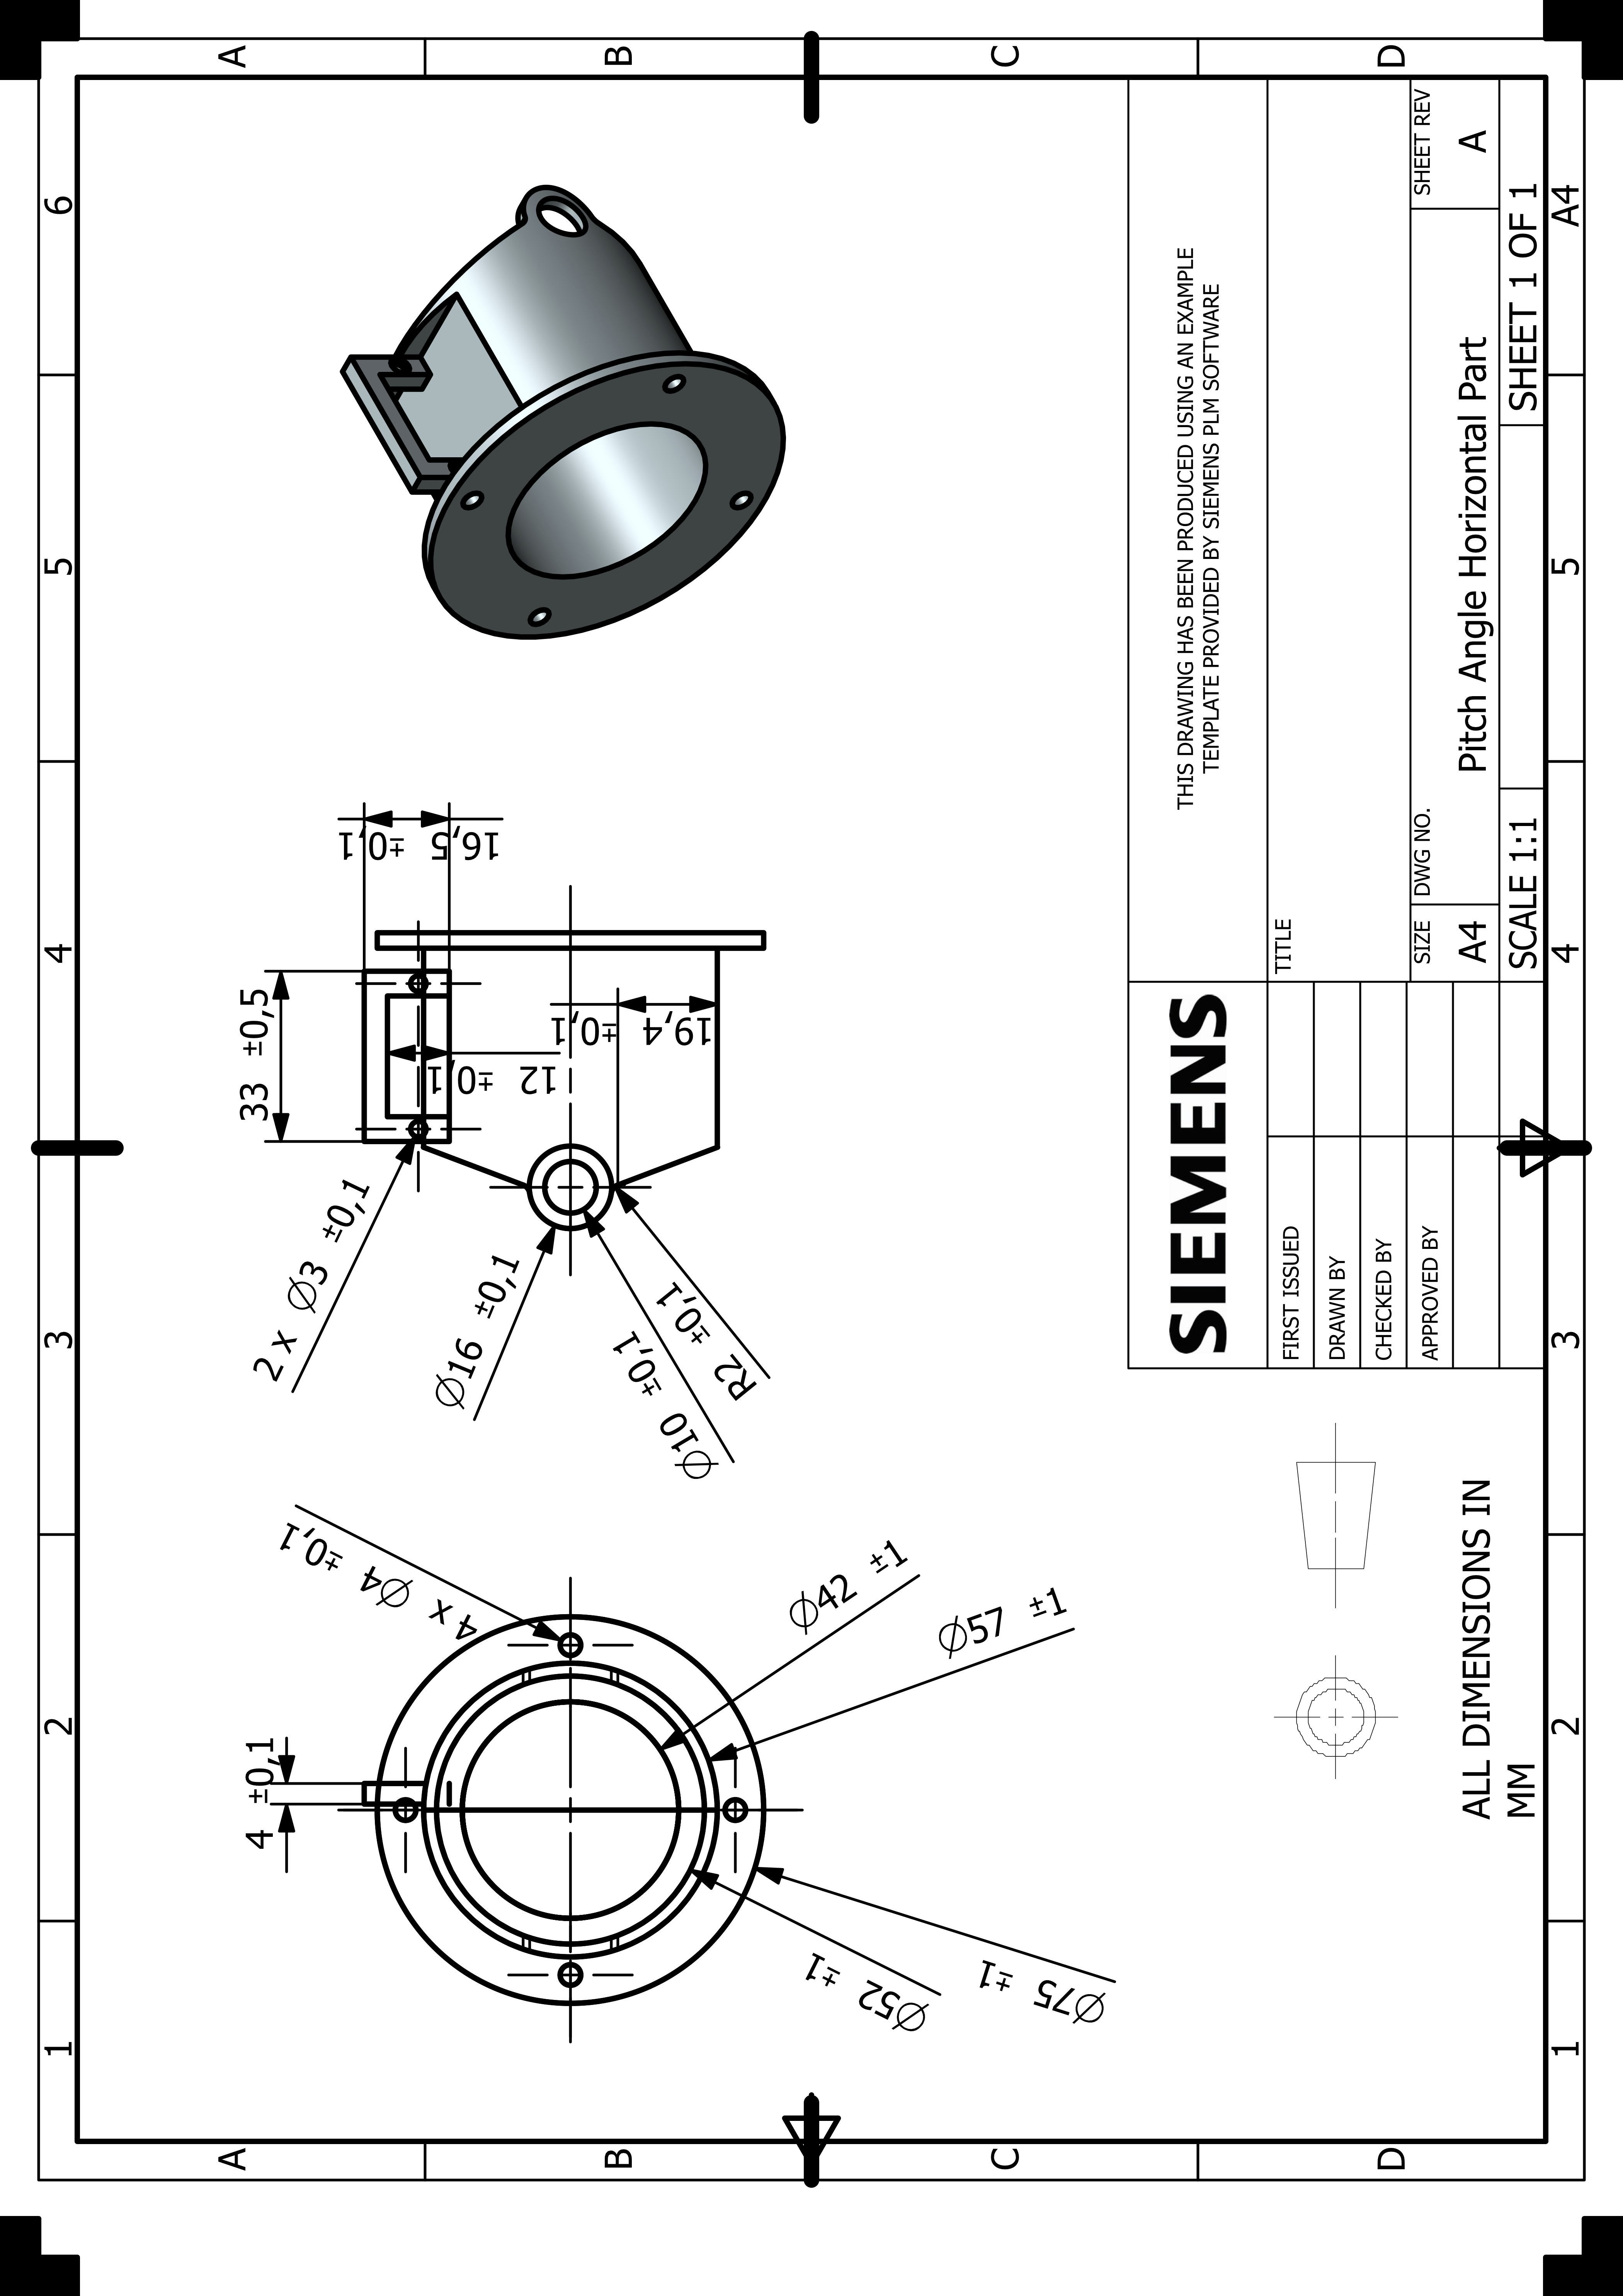
\includegraphics[width=\textwidth]{HP_Pitch Angle Horizontal Part.png} 
    \caption{Technical drawing of the fixed part for pitch angle}
    \label{fig:technical-drawing}
\end{figure}

\begin{figure}[H]
    \centering
    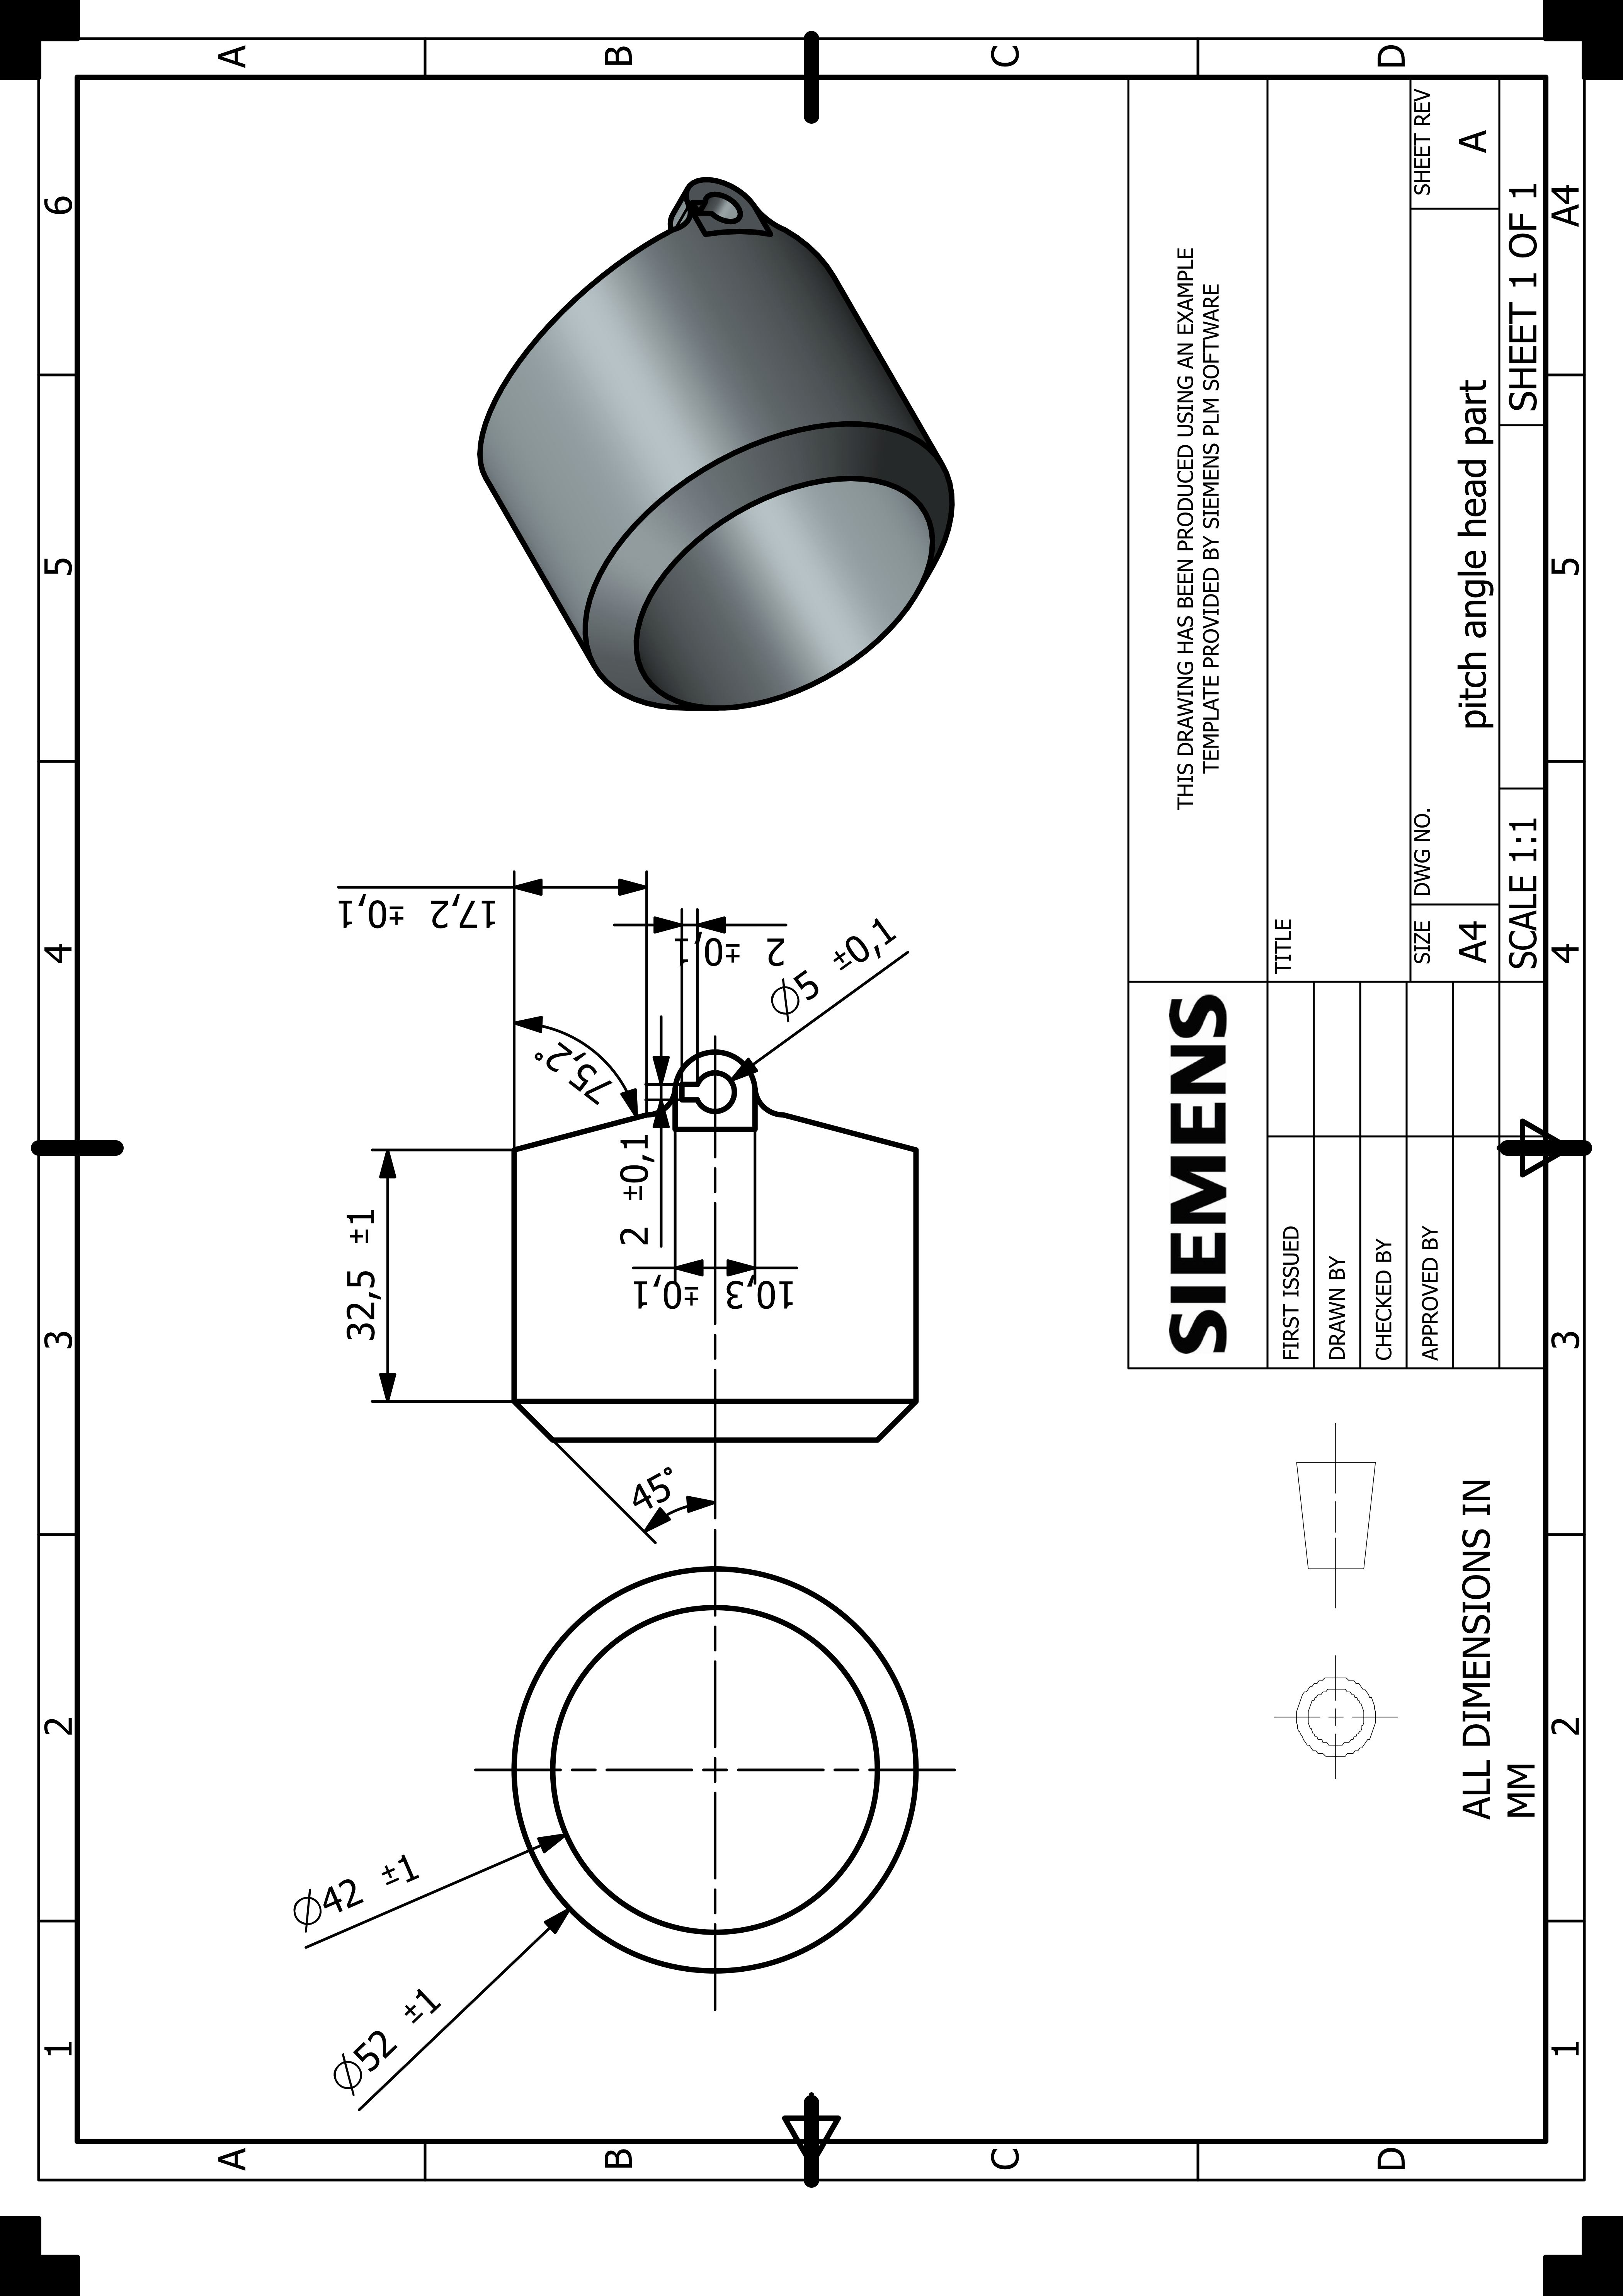
\includegraphics[width=\textwidth]{HP_pitch angle head part.png} 
    \caption{Technical drawing of the moving part for pitch angle}
    \label{fig:technical-drawing}
\end{figure}

\newpage

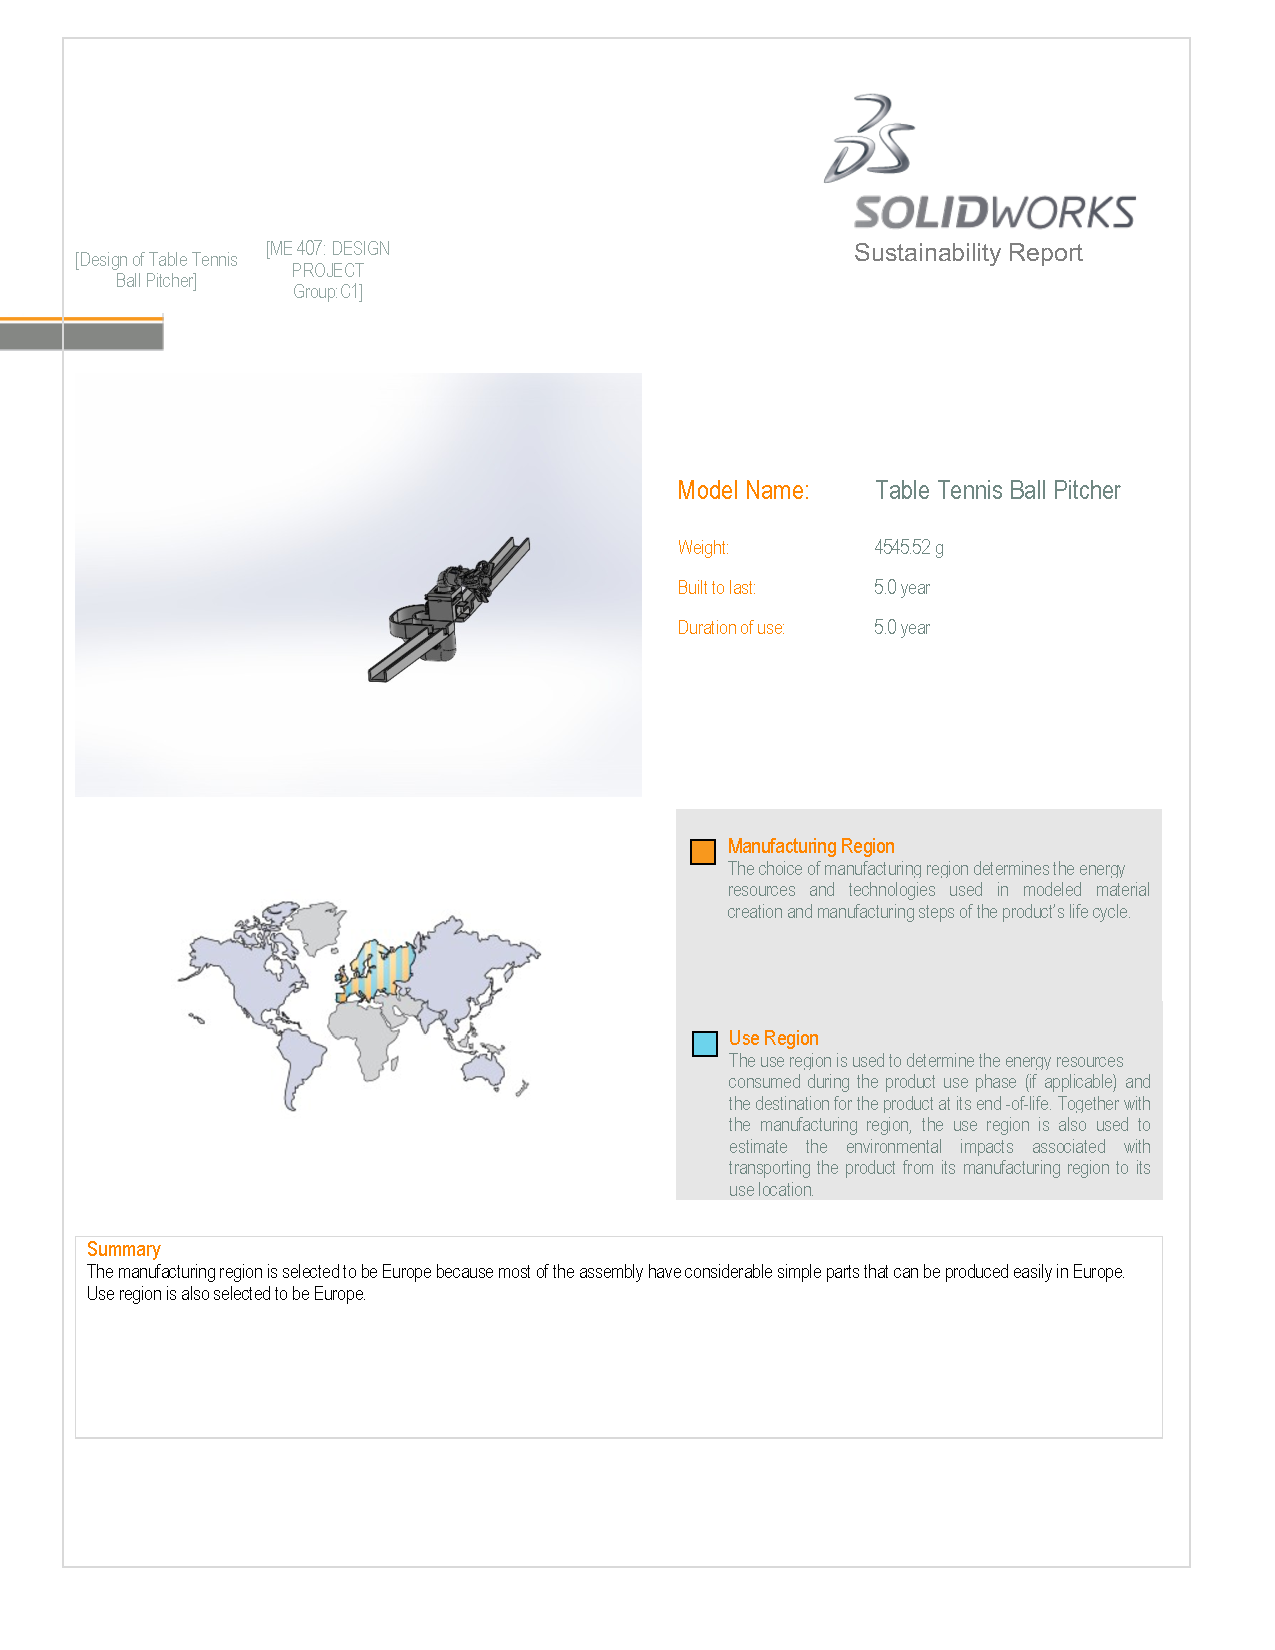
\includepdf[pages=1, pagecommand={\vspace*{-2em}\section{Sustainability Report}}]{sustainability.pdf}

\includepdf[pages=2-]{sustainability.pdf}

\section{Bill of Materials}

\begin{figure}[H]
    \centering
    \includegraphics[width=\textwidth]{Bill of materials 1.png} 
    \caption{Bill of materials to be bought}
    \label{fig:bill-of-materials}
\end{figure}

\begin{figure}[H]
    \centering
    \includegraphics[width=\textwidth]{Bill of materials 2.png} % Replace with your file name
    \caption{Bill of materials to be manufactured}
    \label{fig:bill-of-materials}
\end{figure}
\section{Production Planning}

\begin{center}
\begin{tabular}{|l|l|l|l|}
\hline
\multicolumn{4}{|c|}{\textbf{Production Planning}} \\ \hline
\textbf{Part}               & \textbf{Operations} & \textbf{Location} & \textbf{Date} \\ \hline
Head Pipe                  & 3D printing         & Research Center       & 21.12.2024    \\ \hline
Head Motor Attachment      & 3D printing         & Research Center       & 21.12.2024    \\ \hline
Wheels                     & 3D printing         & Research Center       & 21.12.2024    \\ \hline
Pitch Angle Gear 1         & 3D printing         & Research Center       & 21.12.2024    \\ \hline
Pitch Angle Gear 2         & 3D printing         & Research Center       & 21.12.2024    \\ \hline
Yaw Angle Gear Pair        & 3D printing         & Research Center       & 21.12.2024    \\ \hline
Upper Body Pipe            & 3D printing         & Research Center       & 21.12.2024    \\ \hline
Lower Body Pipe            & 3D printing         & Research Center       & 21.12.2024    \\ \hline
Maltese wheel              & 3D printing         & Research Center       & 21.12.2024    \\ \hline
Groove                     & Cutting             & 407 lab            & 21.12.2024          \\ \hline
\end{tabular}
\end{center}


\section{Route Sheets}

\begin{figure}[H]
    \centering
    \includegraphics[width=\textwidth]{Slide8.jpeg} 
    \label{fig:route-sheet}
\end{figure}

\begin{figure}[H]
    \centering
    \includegraphics[width=\textwidth]{Slide9.jpeg} 
    \label{fig:route-sheet}
\end{figure}

\begin{figure}[H]
    \centering
    \includegraphics[width=\textwidth]{Slide10.jpeg} 
    \label{fig:route-sheet}
\end{figure}

\begin{figure}[H]
    \centering
    \includegraphics[width=\textwidth]{Slide11.jpeg} 
    \label{fig:route-sheet}
\end{figure}

\begin{figure}[H]
    \centering
    \includegraphics[width=\textwidth]{Slide12.jpeg} 
    \caption{Route sheets for the components}
    \label{fig:route-sheet}
\end{figure}

\section{Cost Analysis}

\begin{table}[H]
\centering
\begin{tabular}{|c|l|c|c|l|}
\hline
\textbf{PART NO.} & \textbf{PART NAME}            & \textbf{QUANTITY} & \textbf{COST (\$)} & \textbf{MATERIAL}      \\ \hline
1  & Launcher BLDC Motors       & 3 & 30    & -                  \\ \hline
2  & ESC for BLDC Motors        & 3 & 21    & -                  \\ \hline
3  & Pitch Angle Gear Servo Motor & 1 & 2.5   & -                  \\ \hline
4  & Yaw Angle Gear Servo Motor & 1 & 2.5   & -                  \\ \hline
5  & Bearing Pair               & 2 & 8     & -                  \\ \hline
6  & Maltese Wheel Stepper Motor & 1 & 7     & -                  \\ \hline
7  & Stepper Motor Controller   & 1 & 2     & -                  \\ \hline
8  & Table Attachment Clamp     & 2 & 4.5   & Aluminium                  \\ \hline
9  & Net                        & 1 & 10    & Plastic                  \\ \hline
10 & Head Pipe                  & 1 & 0.43  & ABS                \\ \hline
11 & Head Motor Attachments     & 3 & 0.43  & ABS                \\ \hline
12 & Wheels                     & 3 & 1.4   & ABS                \\ \hline
13 & Pitch Angle Gear Pair      & 1 & 0.7   & ABS                \\ \hline
14 & Yaw Angle Gear Pair        & 1 & 1     & ABS                \\ \hline
15 & Upper Part of Pipe         & 1 & 1.5   & Polycarbonate      \\ \hline
16 & Lower Part of Pipe         & 1 & 2     & Polycarbonate      \\ \hline
17 & Maltese Wheel              & 2 & 0.2   & ABS                \\ \hline
18 & Groove                     & 1 & 2     & Polycarbonate      \\ \hline
\multicolumn{3}{|r|}{\textbf{Total Cost}} & \textbf{97.16} & - \\ \hline
\end{tabular}
\caption{Cost analysis}
\end{table}

\section{Control Schematic}
\begin{figure}[H]
    \centering
    \includegraphics[width=0.9\textwidth]{test.png} 
    \caption{Control schematic of the system}
    \label{fig:control-scheme}
\end{figure}


\end{appendices}
\end{document}